\documentclass[twoside]{article}

\usepackage{aistats2021}
% If your paper is accepted, change the options for the package
% aistats2021 as follows:
%
%\usepackage[accepted]{aistats2021}
%
% This option will print headings for the title of your paper and
% headings for the authors names, plus a copyright note at the end of
% the first column of the first page.

% If you set papersize explicitly, activate the following three lines:
%\special{papersize = 8.5in, 11in}
%\setlength{\pdfpageheight}{11in}
%\setlength{\pdfpagewidth}{8.5in}

% If you use natbib package, activate the following three lines:
\usepackage[round]{natbib}
\renewcommand{\bibname}{References}
\renewcommand{\bibsection}{\subsubsection*{\bibname}}
\usepackage{hyperref}

\usepackage{todonotes}
\usepackage[margin=2.5cm]{geometry}
\usepackage{multirow}
\usepackage{textcomp}
\usepackage{fancyvrb}
\usepackage{todo}



\providecommand{\tightlist}{%
  \setlength{\itemsep}{0pt}\setlength{\parskip}{0pt}}

% If you use BibTeX in apalike style, activate the following line:
%\bibliographystyle{apalike}

\begin{document}

% If your paper is accepted and the title of your paper is very long,
% the style will print as headings an error message. Use the following
% command to supply a shorter title of your paper so that it can be
% used as headings.
%
%\runningtitle{I use this title instead because the last one was very long}

% If your paper is accepted and the number of authors is large, the
% style will print as headings an error message. Use the following
% command to supply a shorter version of the authors names so that
% they can be used as headings (for example, use only the surnames)
%
%\runningauthor{Surname 1, Surname 2, Surname 3, ...., Surname n}

\twocolumn[
\aistatstitle{Inconsistency in Conference Peer Review: Revisiting the NeurIPS Experiment}
\aistatsauthor{Neil D. Lawrence \And Corinna Cortes}
\aistatsaddress{University of Cambridge \And  Google Research, New York}
]

\begin{abstract}
    In this paper we revisit the NeurIPS experiment that examined
inconsistency in conference peer review. We determine that the
underlying cause of inconsistency in the reviews was subjectivity in the
reviewers' quality scores: after score calibration 50\% of the variation
in reviewer scores was subjective in origin. Further, with seven years
passing since the experiment we find that for \emph{accepted} papers,
there is no correlation between quality scores and impact of the paper
as measured as a function of citation count. We trace the fate of
rejected papers, recovering where these papers were eventually
published. For these papers we find a correlation between quality scores
and impact. We conclude that the reviewing process for the 2014
conference was good for identifying poor papers, but poor for
identifying good papers. We give some suggestions for improving the
reviewing process but also warn against removing the subjective element.
Finally, we suggest that the real conclusion of the experiment is that
the community should place less onus on the notion of `top tier
conference publications' when assessing the quality of individual
researchers.
\end{abstract}

\hypertarget{introduction}{%
\section{Introduction}\label{introduction}}

In 2014 the Program Chairs of the NeurIPS conference, Corinna Cortes
and Neil Lawrence, implemented the NeurIPS experiment. The experiment
was designed to assess the consistency of the conference peer
reviewing process. From the conference 10\% of the papers were
randomly chosen to be reviewed by two independent program
committees. The objective was to determine if decision making was
consistent across these two committees.  The results showed that the
decisions between the two committees were 74\% consistent as compared
with a random committee that would have been 62.5\% consistent. While
the review process can be shown to be significantly better than a
random committee (see Appendix \ref{a-random-committee-25} in the
supplementary material for an analysis), the reaction from some in the
community was on of surprise (see Appendix
\ref{reaction-after-experiment} in the supplementary material for an
overview of the reaction). In particular the two committees were only
around 50\% consistent about which papers were selected to appear at
the conference. Researchers realized, that if the review process had
been independently rerun, half the papers published at the conference
would have been different.

We explore these numbers further in three ways. First, we use the fact
that reviewer scores underwent a calibration process during the
conference. This process was focused on eliminating bias in reviewer
scale interpretation, but it also quantifies the subjectivity of
individual reviewer scores. Through a simulation study we demonstrate
that this subjectivity is the at the heart of the inconsistency. Second,
we explored whether these scores correlated with paper citation scores.
Taking citation scores as a proxy for paper impact,\footnote{There are
  problems with using citation scores as a way of assessing impact, see
  e.g. @Neylon-article09 for a discussion, but they have the advantage
  of being an objective, community driven measure and with seven years
  having passed since publication, the papers have had a chance to
  establish themselves.} We collected citation counts for each published
paper from Semantic Scholar,\footnote{\url{https://www.semanticscholar.org/}}
but found no correlation between paper quality scores and the paper's
eventual impact. Finally, we analyzed rejected papers from the
conference. We searched Semantic Scholar for papers with similar titles
by the same lead author in the literature allowing us to track the final
outlet for 680 papers that were rejected by the 2014 NeurIPS conference,
as well as their associated citation counts. For these papers we did
find correlation between quality scores and citation counts.

From these analyses we conclude that inconsistency in the conference
reviewing process is a consequence of the subjectivity in reviewer
assessments. And that in the high scoring range, reviewer quality scores
are not a good proxy for citation impact. However, reviewers seem better
at identifying weaker papers: low scoring papers were (on average) low
impact. Before discussing each of these areas, we first give a brief
reminder of the NeurIPS experiment.

\hypertarget{review-of-the-conference-and-the-experiment}{%
\subsection{Review of the Conference and the
Experiment}\label{review-of-the-conference-and-the-experiment}}

The NeurIPS conference is one of the premier conferences in machine
learning. In 2014 the conference was undergoing a period of rapid
growth. The conference was held in Montreal with 2,581 attendees at the
conference and associated workshops and tutorials. The papers presented
there have proven to be highly influential including breakthrough papers
in unsupervised learning with neural networks as well as papers on
sequence-to-sequence learning for machine translation. These papers have
gone on to have widespread societal impact.

At NeurIPS 2014, each paper was assigned to an Area Chair and at least
three reviewers. Final decisions about papers were made by video
conference between area chairs and the Program Chairs. For more details
on the reviewing process and the timelines involved see Appendix \ref{timeline-for-neurips} in
the supplementary material.

The Program Chairs of the 2014 conference decided to test the
consistency of the peer review process through a randomized experiment.
From the 1,678 submissions they chose 170 papers to undergo review by
two separate committees. Each committee was formed by separating the
reviewing body randomly into two groups, while the Area Chairs were
split manually to ensure proper coverage of expertise in the two bodies.
Each selected paper went through the review process independently.

The results of this process are summarized in Table \ref{table-neurips-experiment-results}, where the
\begin{table}[htb]
\caption{Table showing the results from the two committees as a confusion matrix. Four papers were rejected or withdrawn without review.}
\label{table-neurips-experiment-results}

\begin{tabular}{lc|c|c|}
& & \multicolumn{2}{c}{Committee 1} \\
& & Accept & Reject \\ \hline
\multirow{2}{*}{Committee 2} & Accept & 22 & 22 \\
& Reject & 21 & 101 
\end{tabular}
\end{table}

Cortes and Lawrence also looked at the correlation between the review scores across the two independent committees, a scatter plot of the scores from the committees is shown in Figure \ref{figure-calibrated-quality-correlation}, the Pearson correlation was computed as $\rho=0.55$. For details on the calibration process see Section \ref{reviewer-calibration-and-scoring-inconsistency}.

\begin{figure}[htb]
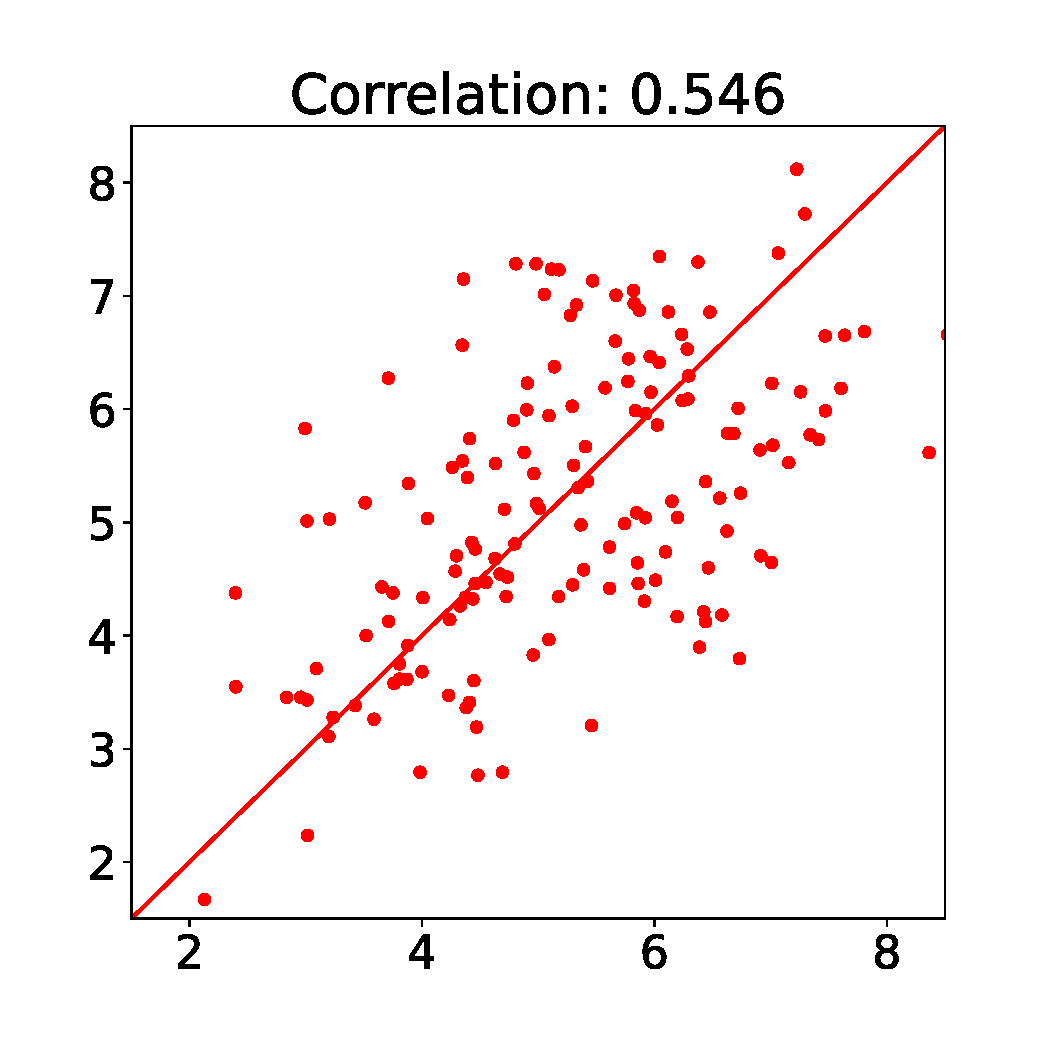
\includegraphics[width=0.60\textwidth]{diagrams/neurips/calibrated-quality-correlation.pdf}

\caption{Correlation between calibrated reviewer scores across the two independent committees. Standard error on the correlation for $n=166$ papers and Gaussian assumptions is $s_r = 0.065$.}
\label{figure-calibrated-quality-correlation}
\end{figure}

During the experiment, the timing of submitted reviews was also tracked. There is evidence that reviews received after the submission deadline, were shorter, typically gave higher scores but with lower confidence (see Appendix \label{effect-of-late-reviews}), but there was insufficient power in the experiment to determine whether this had a significant effect on the correlation across the program committees. 

\section{Results}

Having given an overview of the experiment, we now follow up with our three separate treatments of the results. First we will explore the relationship between the conference calibration and the experimental outcome.

\hypertarget{reviewer-calibration-and-scoring-inconsistency}{%
\subsection{Reviewer Calibration and Scoring Inconsistency}\label{reviewer-calibration-and-scoring-inconsistency}}

NeurIPS papers are evaluated by quality scores on a 10 point Likert
scale (see Appendix \ref{paper-scoring-and-reviewer-instructions}). A
classical challenge with such scales is that they may be interpreted
differently by different reviewers. Since the TK conference, NeurIPS
chairs have often calibrated reviewer scores using scripts of their
own devising. For example, John Platt who chaired the conference in
2006, used a regularized least squares model, this model is written up
in \cite{Platt-calibration12}. The year before us, Zoubin Ghaharamani
and Max Welling used a Bayesian extension of this model
\cite{Ge-bayesian15}. Corinna Cortes and Neil Lawrence also used a
Bayesian variant of the Platt-Burges model, but one that was
formulated as a Gaussian process. We give the details of this approach
in the supplementary material (Appendix \ref{reviewer-calibration}),
but in essence the core of the model is as follows. Each review score
is decomposed into three parts,
$$
y_{i,j} = f_i + b_j + \epsilon_{i, j},
$$
where $y_{i,j}$ is the score from the $j$th reviewer for the $i$th
paper. The score is then decomposed into $f_i$ which is the
\emph{objective} quality of the $i$th paper, i.e. it represents the
portion of the score that is common to all the reviewers. The term
$b_j$ is specific to the $j$th reviewer and it represents an offset or
bias associated with the $j$th reviewer. The idea being that different
reviewers interpret the scale differently. Finally $\epsilon_{i,j}$ is
a \emph{subjective} estimate of the quality of paper $i$ according to
reviewer $j$. It reflects how a specific reviewer's opinion differs
from other reviewers. These differences in opinion may be arising due
to differing expertise or perspective).

The model contains $n$ + $m$ + $n\hat{k}$ parameters where $n=1,678$
is the number of papers, $m=1,474$ is the number of reviewers and
$\hat{k}$ is the average number of reviewers per paper. Given that the
data consists of $n\hat{k}$ reviewing scores, the model is
over-parameterised. The original Platt-Burges model used
regularization to deal with this parameterisation, both
\cite{Ge-bayesian15} and Cortes and Lawrence deal with extra
parameters by allocating them a probability distribution. In the
Cortes and Lawrence case a Gaussian probability results in a latent
variable model that has a marginal likelihood which is jointly
Gaussian, so we have
$$
\mathbf{y} \sim N(\mu \mathbf{1}, \mathbf{K}),
$$
where $\mathbf{y}$ is a vector of stacked scores $\mathbf{1}$ is
the vector of ones and the elements of the covariance function are given
by
$$
k(i,j; k,l) = \delta_{i,k} \alpha_f + \delta_{j,l} \alpha_b + \delta_{i, k}\delta_{j,l} \sigma^2,
$$ where $i$ and $j$ are the index of one paper and reviewer and $k$
and $l$ are the index of a potentially different paper and
reviewer. Three of the parameters of this distribution, $\alpha_f$,
$\alpha_b$, $\sigma^2$ represent the explained variance of the the
score coming from objective quality rating, reviewer offset and
subjective quality rating respectively. As described in the appendix,
the calibrated reviewer score is estimated as the conditional density
of $f_i + \epsilon_{i,j}$. Note that the calibrated reviewer score
\emph{includes} the reviewer's \emph{subjective} opinion about the
paper. See Appendix \ref{reviewer-calibration-model} for more details
on the model as well as code for fitting the model in GPy
\cite{Gpy-20012}. The parameters of the fitted model are given in
Table \ref{fitted-calibration-parameters}.

\begin{table}[htb]
  \label{table-fitted-calibration-parameters}
  \caption{Fitted parameters of the calibration model. The parameters are very well determined as the model is based on around 6,000 reviewer scores. Once the individual reviewer offset, $\alpha_b=0.24$, is removed, the calibrated score $f_i = 1.28$ plus $\epsilon_{i,j}=1.27$ is made up approximately of subjective and objective assessment in roughly equal proportion.} 
  \begin{tabular}{ccc}
    \alpha_f & \alpha _b & \sigma^2 \\
    1.28 & 0.24 & 1.27
  \end{tabular}
\end{table}  

Under the model assumptions we see that calibrated review scores are
made up of subjective and objective opinion in roughly equal
proportions. In other words, 50\% of a typical reviewer's score is
coming from opinion that is particular to that reviewer and \emph{not}
shared with the other reviewers. This figure may seem large, but in
retrospect it is perhaps not surprising. Papers are judged by
subjective criteria such as novelty as well as more objective criteria
such as rigour. The subjectivity of reviewer scores also seems a
sensible starting point to unpick the inconsistency between the two
committees described by the NeurIPS experiment. 


The result is
consistent with the correlation coefficient we computed between the
two independent committees, $\rho = 0.55 \pm 0.065$. Our calibration
model is suggesting that the overall correlation between two
committees would be given by $0.502 = 1.28/(1.28+1.27)$.

To check whether this subjective scoring also explains the
inconsistency in decisions between the two committees, we set up a
simple simulation study. For our simulations, we assumed that each
paper was scored according to the model we've given above and we
estimated the accept consistency through averaging across 100,000
samples. In Figure \ref{figure-consistency-vs-accept-rate} we show the
estimates of the accept consistency as a function of conference accept
rate.

\todo{Neil: this simulation is 50/50, but given that there are four reviewer scores, that are averaged, sholuldn't the simulation be $f__i + \frac{1}{4}\epsilon_{i,j}$?}

\begin{figure}[htb]
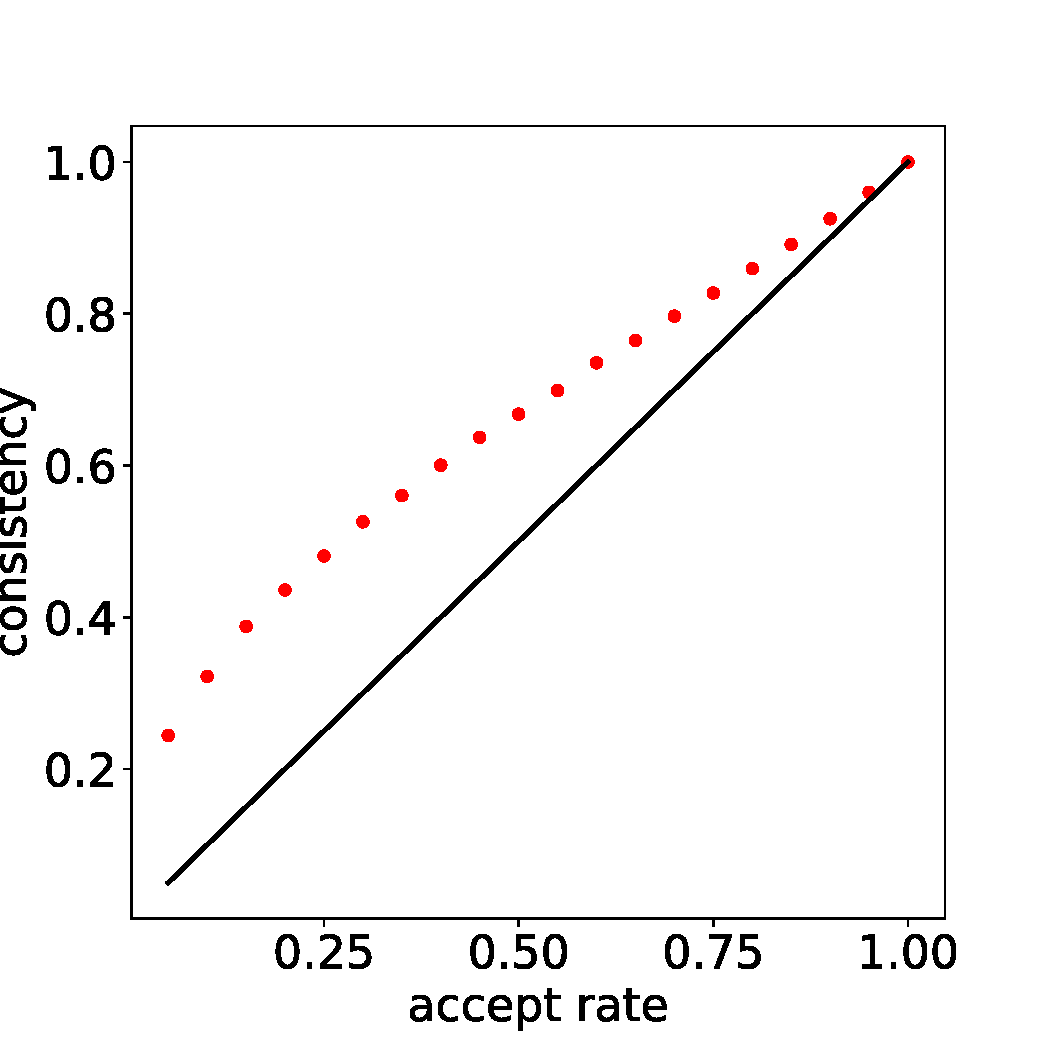
\includegraphics[width=0.50\textwidth]{diagrams/neurips/consistency-vs-accept-rate.pdf}

\caption{Plot of the accept rate versus the accept consistency of
the conference for 50\% subjectivity in a simulation of the conference.}
\label{figure-consistency-vs-accept-rate}
\end{figure}

The estimated accept consistency for a 25\% accept rate is TK, which is consistent with the accept consistency we observed in the experiment.

From these results, we can conclude that the source of inconsistency in the conference can be traced back to subjectivity in the reviews. If we accept our model of review scoring, we can also estimate what this inconsistency is likely to be directly from the model, rather than running the NeurIPS experiment.

It seems self-evident that we might want greater consistency between review committees. After all, if decisions are inconsistent, then how can they be `correct'? While it's true that inconsistency implies incorrectness, the converse is not true. Consistency does not imply correctness. For example, if both committees were to accept all the papers that included the most references, then their decisions would be consistent, but not correct. Indeed, we could argue the converse. Given that we know that incorrect decisions are being made, then do we prefer those errors to be consistent or inconsistent? In this case, we might argue that variation in decision making is a good thing: it prevents particular types of paper being descriminated against.

So, a follow up question would seem to be: how good is the committee at selecting the `right' papers? Unfortunately we don't have a ground truth assessment of what the right papers are. In the absence of this, in the next section, we explore what happened to accepted papers in terms of their citation impact. 

\subsection{Impact of Accepted Papers}

Seven years have now passed since the NeurIPS experiment, and the papers published at the conference have had time to establish themselves. In this section we explore how they faired in terms of \emph{citation impact}.

To determine the citation impact of papers, we searched for each accepted paper from the conference on Semantic Scholar. The Semantic Scholar ID of the papers was recorded and we made use of the Semantic Scholar API to retrieve the number of citing papers. The citation scores were transformed into the citation impact using
$$
\text{citation impact} = \log (1 + \text{number of citations})
$$
which by visual inspection rendered citation scores roughly Gaussian distributed, enabling us to make use of Pearson's rho for correlation measurement.

Our first measurement was to compute the correlation between calibrated quality score and the citation impact. We found \emph{no significant correlation} between those scores. The correlation was computed as $

https://twitter.com/lawrennd/status/1406380063596089346?s=20

\subsection{Fate of Rejected Papers}

\section{Conclusions}

\subsubsection*{Acknowledgements}


\bibliography{revisiting-the-neurips-experiment}

\onecolumn
\aistatstitle{Revisiting the NeurIPS Experiment: \\
Supplementary Materials}
\appendix

\newcommand{\tk}[1]{}
\newcommand{\Amatrix}{\mathbf{A}}
\newcommand{\KL}[2]{\text{KL}\left( #1\,\|\,#2 \right)}
\newcommand{\Kaast}{\kernelMatrix_{\mathbf{ \ast}\mathbf{ \ast}}}
\newcommand{\Kastu}{\kernelMatrix_{\mathbf{ \ast} \inducingVector}}
\newcommand{\Kff}{\kernelMatrix_{\mappingFunctionVector \mappingFunctionVector}}
\newcommand{\Kfu}{\kernelMatrix_{\mappingFunctionVector \inducingVector}}
\newcommand{\Kuast}{\kernelMatrix_{\inducingVector \bf\ast}}
\newcommand{\Kuf}{\kernelMatrix_{\inducingVector \mappingFunctionVector}}
\newcommand{\Kuu}{\kernelMatrix_{\inducingVector \inducingVector}}
\newcommand{\Kuui}{\Kuu^{-1}}
\newcommand{\Qaast}{\mathbf{Q}_{\bf \ast \ast}}
\newcommand{\Qastf}{\mathbf{Q}_{\ast \mappingFunction}}
\newcommand{\Qfast}{\mathbf{Q}_{\mappingFunctionVector \bf \ast}}
\newcommand{\Qff}{\mathbf{Q}_{\mappingFunctionVector \mappingFunctionVector}}
\newcommand{\aMatrix}{\mathbf{A}}
\newcommand{\aScalar}{a}
\newcommand{\aVector}{\mathbf{a}}
\newcommand{\acceleration}{a}
\newcommand{\bMatrix}{\mathbf{B}}
\newcommand{\bScalar}{b}
\newcommand{\bVector}{\mathbf{b}}
\newcommand{\basisFunc}{\phi}
\newcommand{\basisFuncVector}{\boldsymbol{ \basisFunc}}
\newcommand{\basisFunction}{\phi}
\newcommand{\basisLocation}{\mu}
\newcommand{\basisMatrix}{\boldsymbol{ \Phi}}
\newcommand{\basisScalar}{\basisFunction}
\newcommand{\basisVector}{\boldsymbol{ \basisFunction}}
\newcommand{\activationFunction}{\phi}
\newcommand{\activationMatrix}{\boldsymbol{ \Phi}}
\newcommand{\activationScalar}{\basisFunction}
\newcommand{\activationVector}{\boldsymbol{ \basisFunction}}
\newcommand{\bigO}{\mathcal{O}}
\newcommand{\binomProb}{\pi}
\newcommand{\cMatrix}{\mathbf{C}}
\newcommand{\cbasisMatrix}{\hat{\boldsymbol{ \Phi}}}
\newcommand{\cdataMatrix}{\hat{\dataMatrix}}
\newcommand{\cdataScalar}{\hat{\dataScalar}}
\newcommand{\cdataVector}{\hat{\dataVector}}
\newcommand{\centeredKernelMatrix}{\mathbf{ \MakeUppercase{\centeredKernelScalar}}}
\newcommand{\centeredKernelScalar}{b}
\newcommand{\centeredKernelVector}{\centeredKernelScalar}
\newcommand{\centeringMatrix}{\mathbf{H}}
\newcommand{\chiSquaredDist}[2]{\chi_{#1}^{2}\left(#2\right)}
\newcommand{\chiSquaredSamp}[1]{\chi_{#1}^{2}}
\newcommand{\conditionalCovariance}{\boldsymbol{ \Sigma}}
\newcommand{\coregionalizationMatrix}{\mathbf{B}}
\newcommand{\coregionalizationScalar}{b}
\newcommand{\coregionalizationVector}{\mathbf{ \coregionalizationScalar}}
\newcommand{\covDist}[2]{\text{cov}_{#2}\left(#1\right)}
\newcommand{\covSamp}[1]{\text{cov}\left(#1\right)}
\newcommand{\covarianceScalar}{c}
\newcommand{\covarianceVector}{\mathbf{ \covarianceScalar}}
\newcommand{\covarianceMatrix}{\mathbf{C}}
\newcommand{\covarianceMatrixTwo}{\boldsymbol{ \Sigma}}
\newcommand{\croupierScalar}{s}
\newcommand{\croupierVector}{\mathbf{ \croupierScalar}}
\newcommand{\croupierMatrix}{\mathbf{ \MakeUppercase{\croupierScalar}}}
\newcommand{\dataDim}{p}
\newcommand{\dataIndex}{i}
\newcommand{\dataIndexTwo}{j}
\newcommand{\dataMatrix}{\mathbf{Y}}
\newcommand{\dataScalar}{y}
\newcommand{\dataSet}{\mathcal{D}}
\newcommand{\dataStd}{\sigma}
\newcommand{\dataVector}{\mathbf{ \dataScalar}}
\newcommand{\decayRate}{d}
\newcommand{\degreeMatrix}{\mathbf{ \MakeUppercase{\degreeScalar}}}
\newcommand{\degreeScalar}{d}
\newcommand{\degreeVector}{\mathbf{ \degreeScalar}}
\newcommand{\diag}[1]{\text{diag}\left(#1\right)}
\newcommand{\diagonalMatrix}{\mathbf{D}}
\newcommand{\diff}[2]{\frac{\text{d}#1}{\text{d}#2}}
\newcommand{\diffTwo}[2]{\frac{\text{d}^2#1}{\text{d}#2^2}}
\newcommand{\displacement}{x}
\newcommand{\displacementVector}{\textbf{\displacement}}
\newcommand{\distanceMatrix}{\mathbf{ \MakeUppercase{\distanceScalar}}}
\newcommand{\distanceScalar}{d}
\newcommand{\distanceVector}{\mathbf{ \distanceScalar}}
\newcommand{\eigenvaltwo}{\ell}
\newcommand{\eigenvaltwoMatrix}{\mathbf{L}}
\newcommand{\eigenvaltwoVector}{\mathbf{l}}
\newcommand{\eigenvalue}{\lambda}
\newcommand{\eigenvalueMatrix}{\boldsymbol{ \Lambda}}
\newcommand{\eigenvalueVector}{\boldsymbol{ \lambda}}
\newcommand{\eigenvector}{\mathbf{ \eigenvectorScalar}}
\newcommand{\eigenvectorMatrix}{\mathbf{U}}
\newcommand{\eigenvectorScalar}{u}
\newcommand{\eigenvectwo}{\mathbf{v}}
\newcommand{\eigenvectwoMatrix}{\mathbf{V}}
\newcommand{\eigenvectwoScalar}{v}
\newcommand{\entropy}[1]{\mathcal{H}\left(#1\right)}
\newcommand{\errorFunction}{E}
\newcommand{\expDist}[2]{\left<#1\right>_{#2}}
\newcommand{\expSamp}[1]{\left<#1\right>}
\newcommand{\expectation}[1]{\left\langle #1 \right\rangle }
\newcommand{\expectationDist}[2]{\left\langle #1 \right\rangle _{#2}}
\newcommand{\expectedDistanceMatrix}{\mathcal{D}}
\newcommand{\eye}{\mathbf{I}}
\newcommand{\fantasyDim}{r}
\newcommand{\fantasyMatrix}{\mathbf{ \MakeUppercase{\fantasyScalar}}}
\newcommand{\fantasyScalar}{z}
\newcommand{\fantasyVector}{\mathbf{ \fantasyScalar}}
\newcommand{\featureStd}{\varsigma}
\newcommand{\gammaCdf}[3]{\mathcal{GAMMA CDF}\left(#1|#2,#3\right)}
\newcommand{\gammaDist}[3]{\mathcal{G}\left(#1|#2,#3\right)}
\newcommand{\gammaSamp}[2]{\mathcal{G}\left(#1,#2\right)}
\newcommand{\gaussianDist}[3]{\mathcal{N}\left(#1|#2,#3\right)}
\newcommand{\gaussianSamp}[2]{\mathcal{N}\left(#1,#2\right)}
\newcommand{\uniformDist}[3]{\mathcal{U}\left(#1|#2,#3\right)}
\newcommand{\uniformSamp}[2]{\mathcal{U}\left(#1,#2\right)}
\newcommand{\given}{|}
\newcommand{\half}{\frac{1}{2}}
\newcommand{\heaviside}{H}
\newcommand{\hiddenMatrix}{\mathbf{ \MakeUppercase{\hiddenScalar}}}
\newcommand{\hiddenScalar}{h}
\newcommand{\hiddenVector}{\mathbf{ \hiddenScalar}}
\newcommand{\identityMatrix}{\eye}
\newcommand{\inducingInputScalar}{z}
\newcommand{\inducingInputVector}{\mathbf{ \inducingInputScalar}}
\newcommand{\inducingInputMatrix}{\mathbf{Z}}
\newcommand{\inducingScalar}{u}
\newcommand{\inducingVector}{\mathbf{ \inducingScalar}}
\newcommand{\inducingMatrix}{\mathbf{U}}
\newcommand{\inlineDiff}[2]{\text{d}#1/\text{d}#2}
\newcommand{\inputDim}{q}
\newcommand{\inputMatrix}{\mathbf{X}}
\newcommand{\inputScalar}{x}
\newcommand{\inputSpace}{\mathcal{X}}
\newcommand{\inputVals}{\inputVector}
\newcommand{\inputVector}{\mathbf{ \inputScalar}}
\newcommand{\iterNum}{k}
\newcommand{\kernel}{\kernelScalar}
\newcommand{\kernelMatrix}{\mathbf{K}}
\newcommand{\kernelScalar}{k}
\newcommand{\kernelVector}{\mathbf{ \kernelScalar}}
\newcommand{\kff}{\kernelScalar_{\mappingFunction \mappingFunction}}
\newcommand{\kfu}{\kernelVector_{\mappingFunction \inducingScalar}}
\newcommand{\kuf}{\kernelVector_{\inducingScalar \mappingFunction}}
\newcommand{\kuu}{\kernelVector_{\inducingScalar \inducingScalar}}
\newcommand{\lagrangeMultiplier}{\lambda}
\newcommand{\lagrangeMultiplierMatrix}{\boldsymbol{ \Lambda}}
\newcommand{\lagrangian}{L}
\newcommand{\laplacianFactor}{\mathbf{ \MakeUppercase{\laplacianFactorScalar}}}
\newcommand{\laplacianFactorScalar}{m}
\newcommand{\laplacianFactorVector}{\mathbf{ \laplacianFactorScalar}}
\newcommand{\laplacianMatrix}{\mathbf{L}}
\newcommand{\laplacianScalar}{\ell}
\newcommand{\laplacianVector}{\mathbf{ \ell}}
\newcommand{\latentDim}{q}
\newcommand{\latentDistanceMatrix}{\boldsymbol{ \Delta}}
\newcommand{\latentDistanceScalar}{\delta}
\newcommand{\latentDistanceVector}{\boldsymbol{ \delta}}
\newcommand{\latentForce}{f}
\newcommand{\latentFunction}{u}
\newcommand{\latentFunctionVector}{\mathbf{ \latentFunction}}
\newcommand{\latentFunctionMatrix}{\mathbf{ \MakeUppercase{\latentFunction}}}
\newcommand{\latentIndex}{j}
\newcommand{\latentScalar}{z}
\newcommand{\latentVector}{\mathbf{ \latentScalar}}
\newcommand{\latentMatrix}{\mathbf{Z}}
\newcommand{\learnRate}{\eta}
\newcommand{\lengthScale}{\ell}
\newcommand{\rbfWidth}{\ell}
\newcommand{\likelihoodBound}{\mathcal{L}}
\newcommand{\likelihoodFunction}{L}
\newcommand{\locationScalar}{\mu}
\newcommand{\locationVector}{\boldsymbol{ \locationScalar}}
\newcommand{\locationMatrix}{\mathbf{M}}
\newcommand{\variance}[1]{\text{var}\left( #1 \right)}
\newcommand{\mappingFunction}{f}
\newcommand{\mappingFunctionMatrix}{\mathbf{F}}
\newcommand{\mappingFunctionTwo}{g}
\newcommand{\mappingFunctionTwoMatrix}{\mathbf{G}}
\newcommand{\mappingFunctionTwoVector}{\mathbf{ \mappingFunctionTwo}}
\newcommand{\mappingFunctionVector}{\mathbf{ \mappingFunction}}
\newcommand{\scaleScalar}{s}
\newcommand{\mappingScalar}{w}
\newcommand{\mappingVector}{\mathbf{ \mappingScalar}}
\newcommand{\mappingMatrix}{\mathbf{W}}
\newcommand{\mappingScalarTwo}{v}
\newcommand{\mappingVectorTwo}{\mathbf{ \mappingScalarTwo}}
\newcommand{\mappingMatrixTwo}{\mathbf{V}}
\newcommand{\maxIters}{K}
\newcommand{\meanMatrix}{\mathbf{M}}
\newcommand{\meanScalar}{\mu}
\newcommand{\meanTwoMatrix}{\mathbf{M}}
\newcommand{\meanTwoScalar}{m}
\newcommand{\meanTwoVector}{\mathbf{ \meanTwoScalar}}
\newcommand{\meanVector}{\boldsymbol{ \meanScalar}}
\newcommand{\mrnaConcentration}{m}
\newcommand{\naturalFrequency}{\omega}
\newcommand{\neighborhood}[1]{\mathcal{N}\left( #1 \right)}
\newcommand{\neilurl}{http://inverseprobability.com/}
\newcommand{\noiseMatrix}{\boldsymbol{ E}}
\newcommand{\noiseScalar}{\epsilon}
\newcommand{\noiseVector}{\boldsymbol{ \epsilon}}
\newcommand{\noiseStd}{\sigma}
\newcommand{\norm}[1]{\left\Vert #1 \right\Vert}
\newcommand{\normalizedLaplacianMatrix}{\hat{\mathbf{L}}}
\newcommand{\normalizedLaplacianScalar}{\hat{\ell}}
\newcommand{\normalizedLaplacianVector}{\hat{\mathbf{ \ell}}}
\newcommand{\numActive}{m}
\newcommand{\numBasisFunc}{m}
\newcommand{\numComponents}{m}
\newcommand{\numComps}{K}
\newcommand{\numData}{n}
\newcommand{\numFeatures}{K}
\newcommand{\numHidden}{h}
\newcommand{\numInducing}{m}
\newcommand{\numLayers}{\ell}
\newcommand{\numNeighbors}{K}
\newcommand{\numSequences}{s}
\newcommand{\numSuccess}{s}
\newcommand{\numTasks}{m}
\newcommand{\numTime}{T}
\newcommand{\numTrials}{S}
\newcommand{\outputIndex}{j}
\newcommand{\paramVector}{\boldsymbol{ \theta}}
\newcommand{\parameterMatrix}{\boldsymbol{ \Theta}}
\newcommand{\parameterScalar}{\theta}
\newcommand{\parameterVector}{\boldsymbol{ \parameterScalar}}
\newcommand{\partDiff}[2]{\frac{\partial#1}{\partial#2}}
\newcommand{\precisionScalar}{j}
\newcommand{\precisionVector}{\mathbf{ \precisionScalar}}
\newcommand{\precisionMatrix}{\mathbf{J}}
\newcommand{\pseudotargetScalar}{\widetilde{y}}
\newcommand{\pseudotargetVector}{\mathbf{ \pseudotargetScalar}}
\newcommand{\pseudotargetMatrix}{\mathbf{ \widetilde{Y}}}
\newcommand{\rank}[1]{\text{rank}\left(#1\right)}
\newcommand{\rayleighDist}[2]{\mathcal{R}\left(#1|#2\right)}
\newcommand{\rayleighSamp}[1]{\mathcal{R}\left(#1\right)}
\newcommand{\responsibility}{r}
\newcommand{\rotationScalar}{r}
\newcommand{\rotationVector}{\mathbf{ \rotationScalar}}
\newcommand{\rotationMatrix}{\mathbf{R}}
\newcommand{\sampleCovScalar}{s}
\newcommand{\sampleCovVector}{\mathbf{ \sampleCovScalar}}
\newcommand{\sampleCovMatrix}{\mathbf{s}}
\newcommand{\scalarProduct}[2]{\left\langle{#1},{#2}\right\rangle}
\newcommand{\sign}[1]{\text{sign}\left(#1\right)}
\newcommand{\sigmoid}[1]{\sigma\left(#1\right)}
\newcommand{\singularvalue}{\ell}
\newcommand{\singularvalueMatrix}{\mathbf{L}}
\newcommand{\singularvalueVector}{\mathbf{l}}
\newcommand{\sorth}{\mathbf{u}}
\newcommand{\spar}{\lambda}
\newcommand{\trace}[1]{\text{tr}\left(#1\right)}
\newcommand{\BasalRate}{B}
\newcommand{\DampingCoefficient}{C}
\newcommand{\DecayRate}{D}
\newcommand{\Displacement}{X}
\newcommand{\LatentForce}{F}
\newcommand{\Mass}{M}
\newcommand{\Sensitivity}{S}
\newcommand{\basalRate}{b}
\newcommand{\dampingCoefficient}{c}
\newcommand{\mass}{m}
\newcommand{\sensitivity}{s}
\newcommand{\springScalar}{\kappa}
\newcommand{\springVector}{\boldsymbol{ \kappa}}
\newcommand{\springMatrix}{\boldsymbol{ \mathcal{K}}}
\newcommand{\tfConcentration}{p}
\newcommand{\tfDecayRate}{\delta}
\newcommand{\tfMrnaConcentration}{f}
\newcommand{\tfVector}{\mathbf{ \tfConcentration}}
\newcommand{\velocity}{v}
\newcommand{\sufficientStatsScalar}{g}
\newcommand{\sufficientStatsVector}{\mathbf{ \sufficientStatsScalar}}
\newcommand{\sufficientStatsMatrix}{\mathbf{G}}
\newcommand{\switchScalar}{s}
\newcommand{\switchVector}{\mathbf{ \switchScalar}}
\newcommand{\switchMatrix}{\mathbf{S}}
\newcommand{\tr}[1]{\text{tr}\left(#1\right)}
\newcommand{\loneNorm}[1]{\left\Vert #1 \right\Vert_1}
\newcommand{\ltwoNorm}[1]{\left\Vert #1 \right\Vert_2}
\newcommand{\onenorm}[1]{\left\vert#1\right\vert_1}
\newcommand{\twonorm}[1]{\left\Vert #1 \right\Vert}
\newcommand{\vScalar}{v}
\newcommand{\vVector}{\mathbf{v}}
\newcommand{\vMatrix}{\mathbf{V}}
\newcommand{\varianceDist}[2]{\text{var}_{#2}\left( #1 \right)}
\newcommand{\vecb}[1]{\left(#1\right):}
\newcommand{\weightScalar}{w}
\newcommand{\weightVector}{\mathbf{ \weightScalar}}
\newcommand{\weightMatrix}{\mathbf{W}}
\newcommand{\weightedAdjacencyMatrix}{\mathbf{A}}
\newcommand{\weightedAdjacencyScalar}{a}
\newcommand{\weightedAdjacencyVector}{\mathbf{ \weightedAdjacencyScalar}}
\newcommand{\onesVector}{\mathbf{1}}
\newcommand{\zerosVector}{\mathbf{0}}


%%%%%%%%%% Start Body %%%%%%%%%%

\definecolor{societyColor}{RGB}{221,221,78}

\definecolor{vulnerabilityColor}{RGB}{78,221,78}

\definecolor{enfranchisementColor}{RGB}{78,221,78}

\definecolor{individualColor}{RGB}{221,78,78}

\hypertarget{introduction}{%
\section{Introduction}\label{introduction}}

The NIPS experiment was an experiment to determine the consistency of
the review process. After receiving papers we selected 10\% that would
be independently rereviewed. The idea was to determine how consistent
the decisions between the two sets of independent papers would be. In
2014 NIPS received 1678 submissions and we selected 170 for the
experiment. These papers are referred to below as `duplicated papers'.

To run the experiment we created two separate committees within the NIPS
program committee. The idea was that the two separate committees would
review each duplicated paper independently and results compared.

\hypertarget{neurips-in-numbers}{%
\subsection{NeurIPS in Numbers}\label{neurips-in-numbers}}

\begin{flushright}
[\href{https://github.com/lawrennd/talks/edit/gh-pages/_neurips/includes/neurips-in-numbers.md}{edit}]
\end{flushright}

In 2014 the NeurIPS conference had 1474 active reviewers (up from 1133
in 2013), 92 area chairs (up from 67 in 2013) and two program chairs,
myself and Corinna Cortes.

The conference received 1678 submissions and presented 414 accepted
papers, of which 20 were presented as talks in the single track session,
62 were presented as spotlights and 331 papers were presented as
posters. Of the 1678 submissions, 19 papers were rejected without
review.

\hypertarget{the-neurips-experiment}{%
\subsection{The NeurIPS Experiment}\label{the-neurips-experiment}}

The objective of the NeurIPS experiment was to determine how consistent
the process of peer review is. One way of phraising this question is to
ask: what would happen to submitted papers in the conference if the
process was independently rerun?

For the 2014 conference, to explore this question, we selected
\(\approx 10\%\) of submitted papers to be reviewed twice, by
independent committees. This led to 170 papers being selected from the
conference for dual reviewing. For these papers the program committee
was divided into two. Reviewers were placed randomly on one side of the
committee or the other. For Program Chairs we also engaged in some
manual selection to ensure we had expert coverage in all the conference
areas on both side of the committee.

\hypertarget{timeline-for-neurips}{%
\subsection{Timeline for NeurIPS}\label{timeline-for-neurips}}

\begin{flushright}
[\href{https://github.com/lawrennd/talks/edit/gh-pages/_neurips/includes/neurips-timeline.md}{edit}]
\end{flushright}

\paragraph{AC recruitment (3 waves)}

Chairing a conference starts with recruitment of the program committee,
which is usually done in a few stages. The primary task is to recruit
the area chairs. We sent out our program committee invites in three
waves.

\begin{itemize}
\tightlist
\item
  17/02/2014
\item
  08/03/2014
\item
  09/04/2014
\end{itemize}

By recruiting area chairs first, you can involve them in recruiting
reviewers. We requested names of reviewers from ACs in two waves.

\begin{itemize}
\tightlist
\item
  25/03/2014
\item
  11/04/2014
\end{itemize}

In 2014, this wasn't enough to obtain the requisite number of reviewers,
so we used additional approaches. These included lists of previous
NeurIPS authors. For each individual we were looking for at least two
previous papers published or papers published at NeurIPS and other
leading ML venues like ICML, AISTATS, COLT, UAI etc. We made extensive
use of \href{https://dblp.uni-trier.de/}{DBLP} for verifying potential
reviewer's publication track record.

\paragraph{Reviewer recruitment}

\begin{itemize}
\tightlist
\item
  14/04/2014
\item
  28/04/2014
\item
  09/05/2014
\item
  10/06/2014 (note this is after deadline \ldots{} lots of area chairs
  asked for reviewers after the deadline!). We invited them en-masse.
\end{itemize}

\paragraph{Decision Making Timeline}

\begin{itemize}
\tightlist
\item
  06/06/2014 Submission Deadline
\item
  12/06/2014 Bidding Open For Area Chairs (this was \emph{delayed} by
  CMT issues)
\item
  17/06/2014 Bidding Open For Reviewers
\item
  01/07/2014 Start Reviewing
\item
  21/07/2014 Reviewing deadline
\item
  04/08/2014 Reviews to Authors
\item
  11/08/2014 Author Rebuttal Due
\item
  25/08/2014 Teleconferences Begin
\item
  30/08/2014 Teleconferences End
\item
  1/09/2014 Preliminary Decisions Made
\item
  9/09/2014 Decisions Sent to Authors
\end{itemize}

\hypertarget{paper-scoring-and-reviewer-instructions}{%
\subsection{Paper Scoring and Reviewer
Instructions}\label{paper-scoring-and-reviewer-instructions}}

\begin{flushright}
[\href{https://github.com/lawrennd/talks/edit/gh-pages/_neurips/includes/paper-scoring.md}{edit}]
\end{flushright}

The instructions to reviewers for the 2014 conference are still
available
\href{https://nips.cc/Conferences/2014/PaperInformation/ReviewerInstructions}{online
here}.

To keep quality of reviews high, we tried to keep load low. We didn't
assign any reviewer more than 5 papers, most reviewers received 4
papers.

\hypertarget{quantitative-evaluation}{%
\subsection{Quantitative Evaluation}\label{quantitative-evaluation}}

Reviewers give a score of between 1 and 10 for each paper. The program
committee will interpret the numerical score in the following way:

\begin{itemize}
\item
  10: Top 5\% of accepted NIPS papers, a seminal paper for the ages.

  I will consider not reviewing for NIPS again if this is rejected.
\item
  9: Top 15\% of accepted NIPS papers, an excellent paper, a strong
  accept.

  I will fight for acceptance.
\item
  8: Top 50\% of accepted NIPS papers, a very good paper, a clear
  accept.

  I vote and argue for acceptance.
\item
  7: Good paper, accept.

  I vote for acceptance, although would not be upset if it were
  rejected.
\item
  6: Marginally above the acceptance threshold.

  I tend to vote for accepting it, but leaving it out of the program
  would be no great loss.
\item
  5: Marginally below the acceptance threshold.

  I tend to vote for rejecting it, but having it in the program would
  not be that bad.
\item
  4: An OK paper, but not good enough. A rejection.

  I vote for rejecting it, although would not be upset if it were
  accepted.
\item
  3: A clear rejection.

  I vote and argue for rejection.
\item
  2: A strong rejection. I'm surprised it was submitted to this
  conference.

  I will fight for rejection.
\item
  1: Trivial or wrong or known. I'm surprised anybody wrote such a
  paper.

  I will consider not reviewing for NIPS again if this is accepted.
\end{itemize}

Reviewers should NOT assume that they have received an unbiased sample
of papers, nor should they adjust their scores to achieve an artificial
balance of high and low scores. Scores should reflect absolute judgments
of the contributions made by each paper.

\hypertarget{impact-score}{%
\subsection{Impact Score}\label{impact-score}}

The impact score was an innovation introduce in 2013 by Ghahramani and
Welling that we retained for 2014. Quoting from the instructions to
reviewers:

\begin{quote}
Independently of the Quality Score above, this is your opportunity to
identify papers that are very different, original, or otherwise
potentially impactful for the NIPS community.

There are two choices:

2: This work is different enough from typical submissions to potentially
have a major impact on a subset of the NIPS community.

1: This work is incremental and unlikely to have much impact even though
it may be technically correct and well executed.

Examples of situations where the impact and quality scores may point in
opposite directions include papers which are technically strong but
unlikely to generate much follow-up research, or papers that have some
flaw (e.g.~not enough evaluation, not citing the right literature) but
could lead to new directions of research.
\end{quote}

\hypertarget{confidence-score}{%
\subsection{Confidence Score}\label{confidence-score}}

Reviewers also give a confidence score between 1 and 5 for each paper.
The program committee will interpret the numerical score in the
following way:

5: The reviewer is absolutely certain that the evaluation is correct and
very familiar with the relevant literature.

4: The reviewer is confident but not absolutely certain that the
evaluation is correct. It is unlikely but conceivable that the reviewer
did not understand certain parts of the paper, or that the reviewer was
unfamiliar with a piece of relevant literature.

3: The reviewer is fairly confident that the evaluation is correct. It
is possible that the reviewer did not understand certain parts of the
paper, or that the reviewer was unfamiliar with a piece of relevant
literature. Mathematics and other details were not carefully checked.

2: The reviewer is willing to defend the evaluation, but it is quite
likely that the reviewer did not understand central parts of the paper.

1: The reviewer's evaluation is an educated guess. Either the paper is
not in the reviewer's area, or it was extremely difficult to understand.

\hypertarget{qualitative-evaluation}{%
\subsection{Qualitative Evaluation}\label{qualitative-evaluation}}

All NIPS papers should be good scientific papers, regardless of their
specific area. We judge whether a paper is good using four criteria; a
reviewer should comment on all of these, if possible:

\begin{itemize}
\item
  Quality

  Is the paper technically sound? Are claims well-supported by
  theoretical analysis or experimental results? Is this a complete piece
  of work, or merely a position paper? Are the authors careful (and
  honest) about evaluating both the strengths and weaknesses of the
  work?
\item
  Clarity

  Is the paper clearly written? Is it well-organized? (If not, feel free
  to make suggestions to improve the manuscript.) Does it adequately
  inform the reader? (A superbly written paper provides enough
  information for the expert reader to reproduce its results.)
\item
  Originality

  Are the problems or approaches new? Is this a novel combination of
  familiar techniques? Is it clear how this work differs from previous
  contributions? Is related work adequately referenced? We recommend
  that you check the proceedings of recent NIPS conferences to make sure
  that each paper is significantly different from papers in previous
  proceedings. Abstracts and links to many of the previous NIPS papers
  are available from http://books.nips.cc
\item
  Significance
\end{itemize}

Are the results important? Are other people (practitioners or
researchers) likely to use these ideas or build on them? Does the paper
address a difficult problem in a better way than previous research? Does
it advance the state of the art in a demonstrable way? Does it provide
unique data, unique conclusions on existing data, or a unique
theoretical or pragmatic approach?

\hypertarget{speculation}{%
\subsection{Speculation}\label{speculation}}

\begin{flushright}
[\href{https://github.com/lawrennd/talks/edit/gh-pages/_neurips/includes/neurips-experiment-speculation.md}{edit}]
\end{flushright}

With the help of \href{http://nicolofusi.com/}{Nicolo Fusi},
\href{http://blog.scicast.org/tag/charles-twardy/}{Charles Twardy} and
the entire Scicast team we launched
\href{https://scicast.org/\#!/questions/1083/trades/create/power}{a
Scicast question}~a week before the results were revealed. The comment
thread for that question already had
\href{https://scicast.org/\#!/questions/1083/comments/power}{an amount
of interesting comment}~before the conference. Just for informational
purposes before we began reviewing Corinna forecast this figure would be
25\% and I forecast it would be 20\%. The box plot summary of
predictions from Scicast is below.

\begin{figure}[htb]
\begin{center}
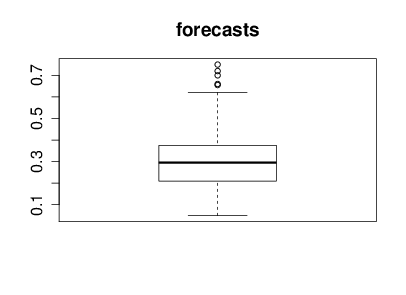
\includegraphics[width=0.40\textwidth]{diagrams/neurips/scicast-forecast.png}
\end{center}


\caption{Summary forecast from those that responded to a scicast question about how consistent the decision making was.}
\label{scicast-forecast}
\end{figure}

\hypertarget{neurips-experiment-results}{%
\subsection{NeurIPS Experiment
Results}\label{neurips-experiment-results}}

\begin{flushright}
[\href{https://github.com/lawrennd/talks/edit/gh-pages/_neurips/includes/neurips-experiment-results.md}{edit}]
\end{flushright}

The final results of the experiment were as follows. From 170 papers 4
had to be withdrawn or were rejected without completing the review
process, for the remainder, the `confusion matrix' for the two
committee's decisions is below.

\begin{tabular}{lccc}
& & \multicolumn{2}{c}{Committee 1} \\
& & Accept & Reject \\
\multirow{2}{*}{Committee 2} & Accept & 22 & 22 \\
& Reject & 21 & 101 
\end{tabular}

4 papers rejected or withdrawn without review.

\hypertarget{summarizing-the-table}{%
\subsection{Summarizing the Table}\label{summarizing-the-table}}

There are a few ways of summarizing the numbers in this table as percent
or probabilities. First of all, the inconsistency, the proportion of
decisions that were not the same across the two committees. The
decisions were inconsistent for 43 out of 166 papers or 0.259 as a
proportion. This number is perhaps a natural way of summarizing the
figures if you are submitting your paper and wish to know an estimate of
what the probability is that your paper would have different decisons
according to the different committes. Secondly, the accept precision: if
you are attending the conference and looking at any given paper, then
you might want to know the probability that the paper would have been
rejected in an independent rerunning of the conference. We can estimate
this for Committee 1's conference as 22/(22 + 22) = 0.5 (50\%) and for
Committee 2's conference as 21/(22+21) = 0.49 (49\%). Averaging the two
estimates gives us 49.5\%. Finally, the reject precision: if your paper
was rejected from the conference, you might like an estimate of the
probability that the same paper would be rejected again if the review
process had been independently rerun. That estimate is 101/(22+101) =
0.82 (82\%) for Committee 1 and 101/(21+101)=0.83 (83\%) for Committee
2, or on average 82.5\%. A final quality estimate might be the ratio of
consistent accepts to consistent rejects, or the agreed accept rate,
22/123 = 0.18 (18\%).

\begin{itemize}
\tightlist
\item
  \emph{inconsistency}: 43/166 = \textbf{0.259}

  \begin{itemize}
  \tightlist
  \item
    proportion of decisions that were not the same
  \end{itemize}
\item
  \emph{accept precision} \(0.5 \times 22/44\) + \(0.5 \times 21/43\) =
  \textbf{0.495}

  \begin{itemize}
  \tightlist
  \item
    probability any accepted paper would be rejected in a rerunning
  \end{itemize}
\item
  \emph{reject precision} = \(0.5\times 101/(22+101)\) +
  \(0.5\times 101/(21 + 101)\) = \textbf{0.175}

  \begin{itemize}
  \tightlist
  \item
    probability any rejected paper would be rejected in a rerunning
  \end{itemize}
\item
  \emph{agreed accept rate} = 22/101 = \textbf{0.218}
\item
  ratio between aggreed accepted papers and agreed rejected papers.
\end{itemize}

\hypertarget{reaction-after-experiment}{%
\subsection{Reaction After Experiment}\label{reaction-after-experiment}}

\begin{flushright}
[\href{https://github.com/lawrennd/talks/edit/gh-pages/_neurips/includes/neurips-experiment-reaction.md}{edit}]
\end{flushright}

There seems to have been a lot of discussion of the result, both at the
conference and on bulletin boards since. Such discussion is to be
encouraged, and for ease of memory, it is worth pointing out that the
approximate proportions of papers in each category can be nicely divided
in to eigths as follows. Accept-Accept 1 in 8 papers, Accept-Reject 3 in
8 papers, Reject-Reject, 5 in 8 papers. This makes the statistics we've
computed above: inconsistency 1 in 4 (25\%) accept precision 1 in 2
(50\%) reject precision 5 in 6 (83\%) and agreed accept rate of 1 in 6
(20\%). This compares with the accept rate of 1 in 4.

\begin{itemize}
\item
  Public reaction after experiment
  \href{http://inverseprobability.com/2015/01/16/blogs-on-the-nips-experiment/}{documented
  here}
\item
  \href{http://inverseprobability.com/2014/07/01/open-data-science/}{Open
  Data Science} (see Heidelberg Meeting)
\item
  NIPS was run in a very open way.
  \href{https://github.com/sods/conference}{Code} and
  \href{http://inverseprobability.com/2014/12/16/the-nips-experiment/}{blog
  posts} all available!
\item
  Reaction triggered by
  \href{http://blog.mrtz.org/2014/12/15/the-nips-experiment.html}{this
  blog post}.
\end{itemize}

Much of the discussion speculates on the number of consistent accepts in
the process (using the main conference accept rate as a proxy). It
therefore produces numbers that don't match ours above. This is because
the computed accept rate of the individual committees is different from
that of the main conference. This could be due to a bias for the
duplicated papers, or statistical sampling error. We look at these
questions below. First, to get the reader primed for thinking about
these numbers we discuss some context for placing these numbers.

\hypertarget{a-random-committee-25}\label{a-random-committee-25}}

\begin{flushright}
[\href{https://github.com/lawrennd/talks/edit/gh-pages/_neurips/includes/neurips-experiment-random-committee.md}{edit}]
\end{flushright}

The first context we can place around the numbers is what would have
happened at the `Random Conference' where we simply accept a quarter of
papers at random. In this NIPS the expected numbers of accepts would
then have been:

Committee 1

Accept

Reject

Committee 2

Accept

10.4 (1 in 16)

31.1 (3 in 16)

Reject

31.1 (3 in 16)

93.4 (9 in 16)

And for this set up we would expect \emph{inconsistency} of 3 in 8
(37.5\%) \emph{accept precision} of 1 in 4 (25\%) and a \emph{reject
precision} of 3 in 4 (75\%) and a \emph{agreed accept rate} of 1 in 10
(10\%). The actual committee made improvements on these numbers, in
particular the accept precision was markedly better with 50\%: twice as
many consistent accept decisions were made than would be expected if the
process had been performed at random and only around two thirds as many
inconsistent decisions were made as would have been expected if
decisions were made at random. However, we should treat all these
figures with some skepticism until we've performed some estimate of the
uncertainty associated with them.

\hypertarget{stats-for-random-committee}{%
\subsection{Stats for Random
Committee}\label{stats-for-random-committee}}

\begin{itemize}
\tightlist
\item
  For random committee we expect:

  \begin{itemize}
  \tightlist
  \item
    \emph{inconsistency} of 3 in 8 (37.5\%)
  \item
    \emph{accept precision} of 1 in 4 (25\%)
  \item
    \emph{reject precision} of 3 in 4 (75\%) and a
  \item
    \emph{agreed accept rate} of 1 in 10 (10\%).
  \end{itemize}
\end{itemize}

Actual committee's accept precision markedly better with 50\% accept
precision.

\hypertarget{uncertainty-accept-rate}{%
\subsection{Uncertainty: Accept Rate}\label{uncertainty-accept-rate}}

To get a handle on the uncertainty around these numbers we'll start by
making use of the (binomial
distribution){[}http://en.wikipedia.org/wiki/Binomial\_distribution{]}.
First, let's explore the fact that for the overall conference the accept
rate was around 23\%, but for the duplication committees the accept rate
was around 25\%. If we assume decisions are made according to a binomial
distribution, then is the accept rate for the duplicated papers too
high?

Note that for all our accept probability statistics we used as a
denominator the number of papers that were initially sent for review,
rather than the number where a final decision was made by the program
committee. These numbers are different because some papers are withdrawn
before the program committee makes its decision. Most commonly this
occurs after authors have seen their preliminary reviews: for NIPS 2014
we provided preliminary reviews that included paper scores. So for the
official accept probability we use the 170 as denominator. The accept
probabilities were therefore 43 out of 170 papers (25.3\%) for Committee
1 and 44 out of 170 (25.8\%) for Committee 2. This compares with the
overall conference accept rate for papers outside the duplication
process of 349 out of 1508 (23.1\%).

If the true underlying probability of an accept were actually 0.23
independent of the paper, then the probability of generating accepts for
any subset of the papers would be given by a binomial distribution.
Combining across the two committees for the duplicated papers, we see
that 87 papers in total were recommended for accept out of a total of
340 trials. out of 166 trials would be given by a binomial distribution
as depicted below.

\begin{Shaded}
\begin{Highlighting}[]
\ImportTok{import}\NormalTok{ numpy }\ImportTok{as}\NormalTok{ np}
\ImportTok{from}\NormalTok{ scipy.stats }\ImportTok{import}\NormalTok{ binom}
\ImportTok{from}\NormalTok{ IPython.display }\ImportTok{import}\NormalTok{ HTML}
\end{Highlighting}
\end{Shaded}

\begin{figure}[htb]
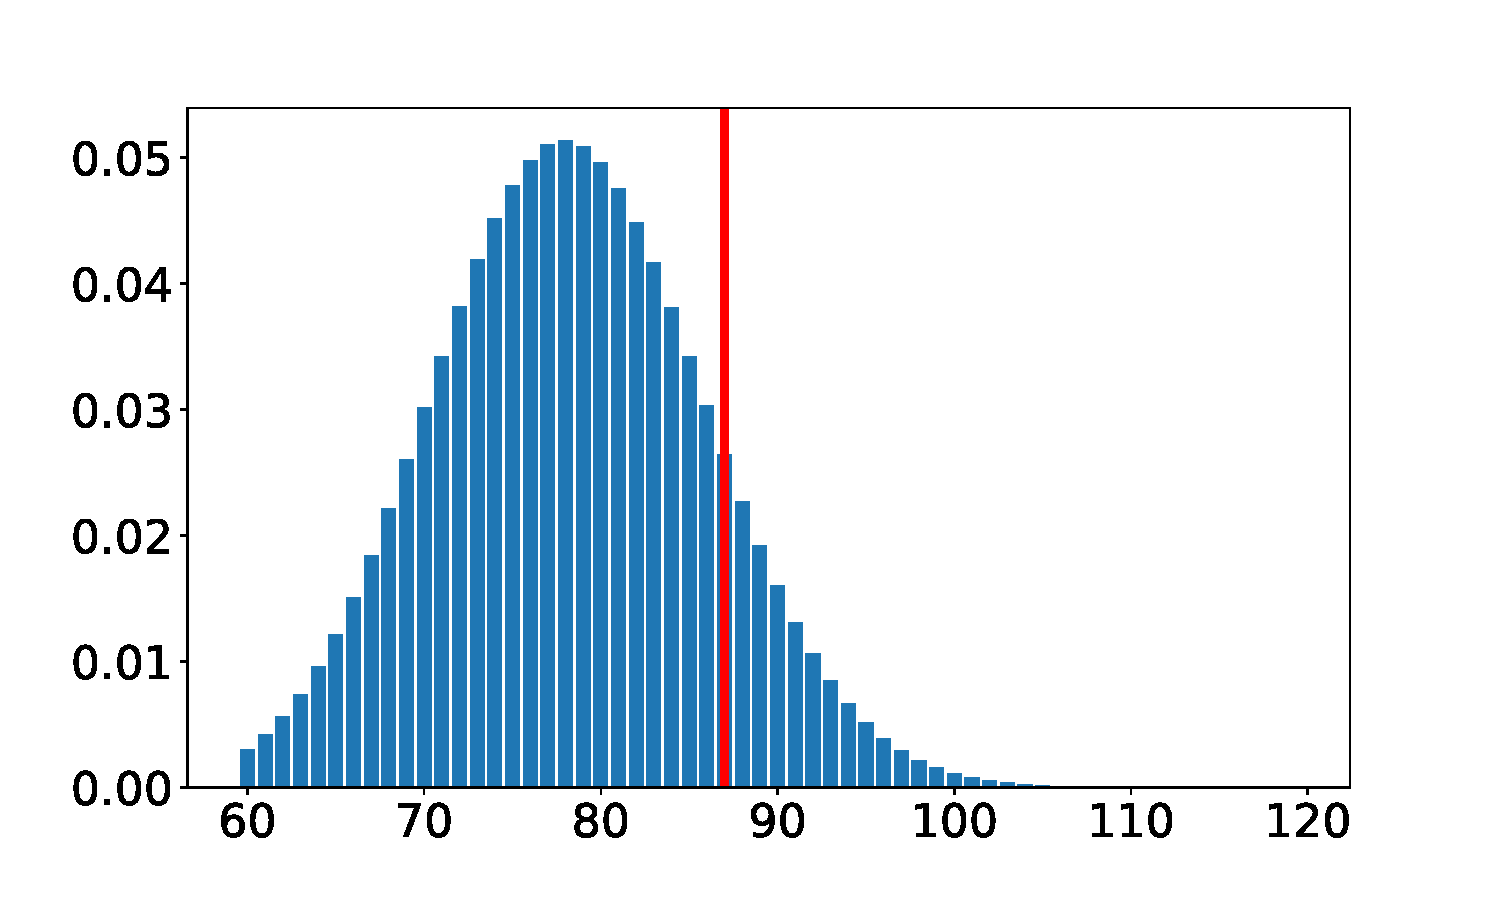
\includegraphics[width=0.70\textwidth]{diagrams/neurips/uncertainty-accept-rate.pdf}


\caption{Number of accepted papers for $p=0.23$.}
\label{uncertainty-accept-rate}
\end{figure}

From the plot, we can see that whilst the accept rate was slightly
higher for duplicated papers it doesn't seem that we can say that it was
statistically significant that it was higher, it falls well within the
probability mass of the Binomial.

Note that Area Chairs knew which papers were duplicates, whereas
reviewers did not. Whilst we stipulated that duplicate papers should not
be any given special treatment, we cannot discount the possibility that
Area Chairs may have given slightly preferential treatment to duplicate
papers.

\hypertarget{uncertainty-accept-precision}{%
\subsection{Uncertainty: Accept
Precision}\label{uncertainty-accept-precision}}

For the accept precision, if we assume that accept decisions were drawn
according to a binomial, then the distribution for consistent accepts is
also binomial. Our best estimate of its parameter is 22/166 = 0.13
(13\%). If we had a binomial distribution with these parameters, then
the distribution of consistent accepts would be as follows.

\begin{itemize}
\tightlist
\item
  How reliable is the consistent accept score?
\end{itemize}

\begin{figure}[htb]
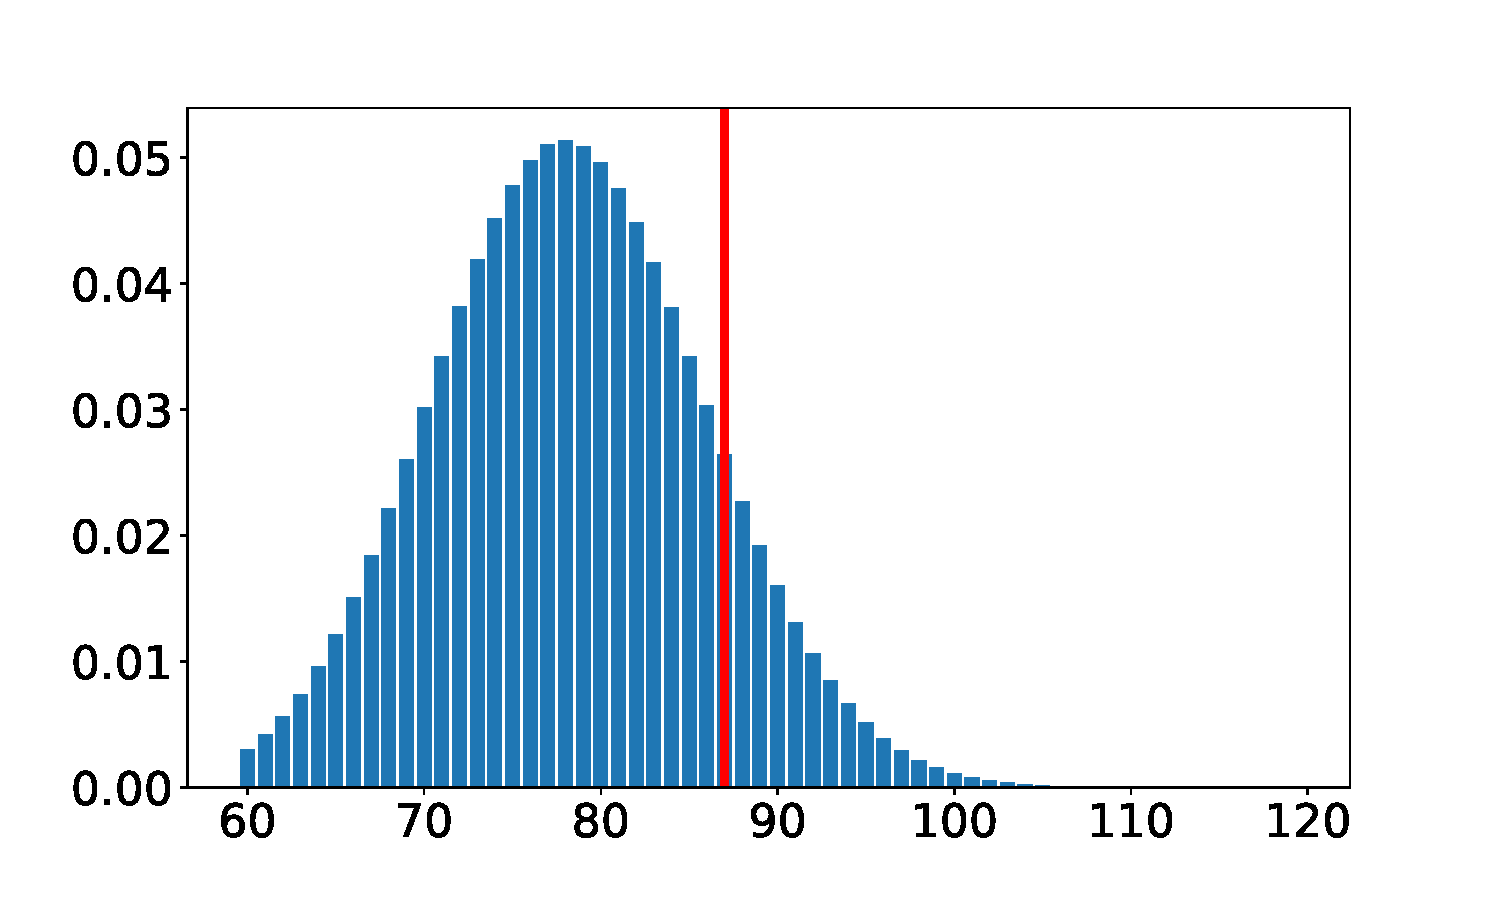
\includegraphics[width=0.70\textwidth]{diagrams/neurips/uncertainty-accept-rate.pdf}


\caption{Number of consistent accepts given $p=0.13$.}
\label{uncertainty-accept-precision}
\end{figure}

We see immediately that there is a lot of uncertainty around this
number, for the scale of the experiment as we have it. This suggests a
more complex analysis is required to extract our estimates with
uncertainty.

\hypertarget{bayesian-analysis}{%
\subsection{Bayesian Analysis}\label{bayesian-analysis}}

Before we start the analysis, it's important to make some statements
about the aims of our modelling here. We will make some simplifying
modelling assumptions for the sake of a model that is understandable. In
particular, we are looking to get a handle on the uncertainty associated
with some of the probabilities associated with the NIPS experiment.
\href{http://inverseprobability.com/2015/01/16/blogs-on-the-nips-experiment/}{Some
preliminary analyses have already been conducted on blogs}. Those
analyses don't have access to information like paper scores etc. For
that reason we also leave out such information in this preliminary
analysis. We will focus only on the summary results from the experiment:
how many papers were consistently accepted, consistently rejected or had
inconsistent decisions. For the moment we disregard the information we
have about paper scores.

In our analysis there are three possible outcomes for each paper:
consistent accept, inconsistent decision and consistent reject. So we
need to perform the analysis with the
\href{http://en.wikipedia.org/wiki/Multinomial_distribution}{multinomial
distribution}. The multinomial is parameterized by the probabilities of
the different outcomes. These are our parameters of interest, we would
like to estimate these probabilities alongside their uncertainties. To
make a Bayesian analysis we place a prior density over these
probabilities, then we update the prior with the observed data, that
gives us a posterior density, giving us an uncertainty associated with
these probabilities.

\hypertarget{prior-density}{%
\subsubsection{Prior Density}\label{prior-density}}

Choice of prior for the multinomial is typically straightforward, the
\href{http://en.wikipedia.org/wiki/Dirichlet_distribution}{Dirichlet
density} is
\href{http://en.wikipedia.org/wiki/Conjugate_prior}{conjugate} and has
the additional advantage that its parameters can be set to ensure it is
\emph{uninformative}, i.e.~uniform across the domain of the prior.
Combination of a multinomial likelihood and a Dirichelt prior is not
new, and in this domain if we were to consider the mean the posterior
density only, then the approach is known as
\href{http://en.wikipedia.org/wiki/Additive_smoothing}{Laplace
smoothing}.

For our model we are assuming for our prior that the probabilities are
drawn from a Dirichlet as follows, \[
p \sim \text{Dir}(\alpha_1, \alpha_2, \alpha_3),
\] with \(\alpha_1=\alpha_2=\alpha_3=1\). The Dirichlet density is
conjugate to the
\href{http://en.wikipedia.org/wiki/Multinomial_distribution}{multinomial
distribution}, and we associate three different outcomes with the
multinomial. For each of the 166 papers we expect to have a consistent
accept (outcome 1), an inconsistent decision (outcome 2) or a consistent
reject (outcome 3). If the counts four outcome 1, 2 and 3 are
represented by \(k_1\), \(k_2\) and \(k_3\) and the associated
probabilities are given by \(p_1\), \(p_2\) and \(p_3\) then our model
is, \begin{align*}
\mathbf{p}|\boldsymbol{\alpha} \sim \text{Dir}(\boldsymbol{\alpha}) \\
\mathbf{k}|\mathbf{p} \sim \text{mult}(\mathbf{p}).
\end{align*} Due to the conjugacy the posterior is tractable and easily
computed as a Dirichlet (see
e.g.~\href{http://www.stat.columbia.edu/~gelman/book/}{Gelman et al}),
where the parameters of the Dirichlet are given by the original vector
from the Dirichlet prior plus the counts associated with each outcome.
\[
\mathbf{p}|\mathbf{k}, \boldsymbol{\alpha} \sim \text{Dir}(\boldsymbol{\alpha} + \mathbf{k})
\] The mean probability for each outcome is then given by, \[
\bar{p}_i = \frac{\alpha_i+k_i}{\sum_{j=1}^3(\alpha_j + k_j)}.
\] and the variance is \[
\mathrm{Var}[p_i] = \frac{(\alpha_i+k_i) (\alpha_0-\alpha_i + n + k_i)}{(\alpha_0+n)^2 (\alpha_0+n+1)},
\] where \(n\) is the number of trials (166 in our case) and
\(\alpha_0 = \sum_{i=1}^3\alpha_i\). This allows us to compute the
expected value of the probabilities and their variances under the
posterior as follows.

\begin{Shaded}
\begin{Highlighting}[]
\KeywordTok{def}\NormalTok{ posterior\_mean\_var(k, alpha):}
    \CommentTok{"""Compute the mean and variance of the Dirichlet posterior."""}
\NormalTok{    alpha\_0 }\OperatorTok{=}\NormalTok{ alpha.}\BuiltInTok{sum}\NormalTok{()}
\NormalTok{    n }\OperatorTok{=}\NormalTok{ k.}\BuiltInTok{sum}\NormalTok{()}
\NormalTok{    m }\OperatorTok{=}\NormalTok{ (k }\OperatorTok{+}\NormalTok{ alpha)}
\NormalTok{    m }\OperatorTok{/=}\NormalTok{ m.}\BuiltInTok{sum}\NormalTok{()}
\NormalTok{    v }\OperatorTok{=}\NormalTok{ (alpha}\OperatorTok{+}\NormalTok{k)}\OperatorTok{*}\NormalTok{(alpha\_0 }\OperatorTok{{-}}\NormalTok{ alpha }\OperatorTok{+}\NormalTok{ n }\OperatorTok{+}\NormalTok{ k)}\OperatorTok{/}\NormalTok{((alpha\_0}\OperatorTok{+}\NormalTok{n)}\OperatorTok{**}\DecValTok{2}\OperatorTok{*}\NormalTok{(alpha\_0}\OperatorTok{+}\NormalTok{n}\OperatorTok{+}\DecValTok{1}\NormalTok{))}
    \ControlFlowTok{return}\NormalTok{ m, v}

\NormalTok{k }\OperatorTok{=}\NormalTok{ np.asarray([}\DecValTok{22}\NormalTok{, }\DecValTok{43}\NormalTok{, }\DecValTok{101}\NormalTok{])}
\NormalTok{alpha }\OperatorTok{=}\NormalTok{ np.ones((}\DecValTok{3}\NormalTok{,))}
\NormalTok{m, v }\OperatorTok{=}\NormalTok{ posterior\_mean\_var(k, alpha)}
\NormalTok{outcome }\OperatorTok{=}\NormalTok{ [}\StringTok{\textquotesingle{}consistent accept\textquotesingle{}}\NormalTok{, }\StringTok{\textquotesingle{}inconsistent decision\textquotesingle{}}\NormalTok{, }\StringTok{\textquotesingle{}consistent reject\textquotesingle{}}\NormalTok{]}
\ControlFlowTok{for}\NormalTok{ i }\KeywordTok{in} \BuiltInTok{range}\NormalTok{(}\DecValTok{3}\NormalTok{):}
\NormalTok{    display(HTML(}\StringTok{"\textless{}h4\textgreater{}Probability of "} \OperatorTok{+}\NormalTok{ outcome[i] }\OperatorTok{+}\StringTok{\textquotesingle{} \textquotesingle{}} \OperatorTok{+} \BuiltInTok{str}\NormalTok{(m[i]) }\OperatorTok{+}  \StringTok{"+/{-}"} \OperatorTok{+} \BuiltInTok{str}\NormalTok{(}\DecValTok{2}\OperatorTok{*}\NormalTok{np.sqrt(v[i])) }\OperatorTok{+} \StringTok{"\textless{}/h4\textgreater{}"}\NormalTok{))}
\end{Highlighting}
\end{Shaded}

So we have a probability of consistent accept as \(0.136 \pm 0.06\), the
probability of inconsistent decision as \(0.260 \pm 0.09\) and
probability of consistent reject as \(0.60 \pm 0.15\). Recall that if
we'd selected papers at random (with accept rate of 1 in 4) then these
values would have been 1 in 16 (0.0625), 3 in 8 (0.375) and 9 in 16
(0.5625).

The other values we are interested in are the accept precision, reject
precision and the agreed accept rate. Computing the probability density
for these statistics is complex, because it involves
\href{http://en.wikipedia.org/wiki/Ratio_distribution}{Ratio
Distributions}. However, we can use Monte Carlo to estimate the expected
accept precision, reject precision and agreed accept rate as well as
their variances. We can use these results to give us error bars and
histograms of these statistics.

\begin{Shaded}
\begin{Highlighting}[]
\KeywordTok{def}\NormalTok{ sample\_precisions(k, alpha, num\_samps):}
    \CommentTok{"""Helper function to sample from the posterior distibution of accept, }
\CommentTok{    reject and inconsistent probabilities and compute other statistics of interest }
\CommentTok{    from the samples."""}

\NormalTok{    k }\OperatorTok{=}\NormalTok{ np.random.dirichlet(k}\OperatorTok{+}\NormalTok{alpha, size}\OperatorTok{=}\NormalTok{num\_samps)}
    \CommentTok{\# Factors of 2 appear because inconsistent decisions }
    \CommentTok{\# are being accounted for across both committees.}
\NormalTok{    ap }\OperatorTok{=} \DecValTok{2}\OperatorTok{*}\NormalTok{k[:, }\DecValTok{0}\NormalTok{]}\OperatorTok{/}\NormalTok{(}\DecValTok{2}\OperatorTok{*}\NormalTok{k[:, }\DecValTok{0}\NormalTok{]}\OperatorTok{+}\NormalTok{k[:, }\DecValTok{1}\NormalTok{])}
\NormalTok{    rp }\OperatorTok{=} \DecValTok{2}\OperatorTok{*}\NormalTok{k[:, }\DecValTok{2}\NormalTok{]}\OperatorTok{/}\NormalTok{(k[:, }\DecValTok{1}\NormalTok{]}\OperatorTok{+}\DecValTok{2}\OperatorTok{*}\NormalTok{k[:, }\DecValTok{2}\NormalTok{])}
\NormalTok{    aa }\OperatorTok{=}\NormalTok{ k[:, }\DecValTok{0}\NormalTok{]}\OperatorTok{/}\NormalTok{(k[:, }\DecValTok{0}\NormalTok{]}\OperatorTok{+}\NormalTok{k[:, }\DecValTok{2}\NormalTok{])}
    \ControlFlowTok{return}\NormalTok{ ap, rp, aa}

\NormalTok{ap, rp, aa }\OperatorTok{=}\NormalTok{ sample\_precisions(k, alpha, }\DecValTok{10000}\NormalTok{)}
\BuiltInTok{print}\NormalTok{(ap.mean(), }\StringTok{\textquotesingle{}+/{-}\textquotesingle{}}\NormalTok{, }\DecValTok{2}\OperatorTok{*}\NormalTok{np.sqrt(ap.var()))}
\BuiltInTok{print}\NormalTok{(rp.mean(), }\StringTok{\textquotesingle{}+/{-}\textquotesingle{}}\NormalTok{, }\DecValTok{2}\OperatorTok{*}\NormalTok{np.sqrt(rp.var()))}
\BuiltInTok{print}\NormalTok{(aa.mean(), }\StringTok{\textquotesingle{}+/{-}\textquotesingle{}}\NormalTok{, }\DecValTok{2}\OperatorTok{*}\NormalTok{np.sqrt(aa.var()))}
\end{Highlighting}
\end{Shaded}

Giving an accept precision of \(0.51 \pm 0.13\), a reject precision of
\(0.82 \pm 0.05\) and an agreed accept rate of \(0.18 \pm 0.07\). Note
that the `random conference' values of 1 in 4 for accept precision and 3
in 4 for reject decisions are outside the two standard deviation error
bars. If it is preferred medians and percentiles could also be computed
from the samples above, but as we will see when we histogram the results
the densities look broadly symmetric, so this is unlikely to have much
effect.

\hypertarget{histogram-of-monte-carlo-results}{%
\subsubsection{Histogram of Monte Carlo
Results}\label{histogram-of-monte-carlo-results}}

Just to ensure that the error bars are reflective of the underlying
densities we histogram the Monte Carlo results for accept precision,
reject precision and agreed accept below. Shown on each histogram is a
line representing the result we would get for the `random committee'.

\begin{figure}[htb]
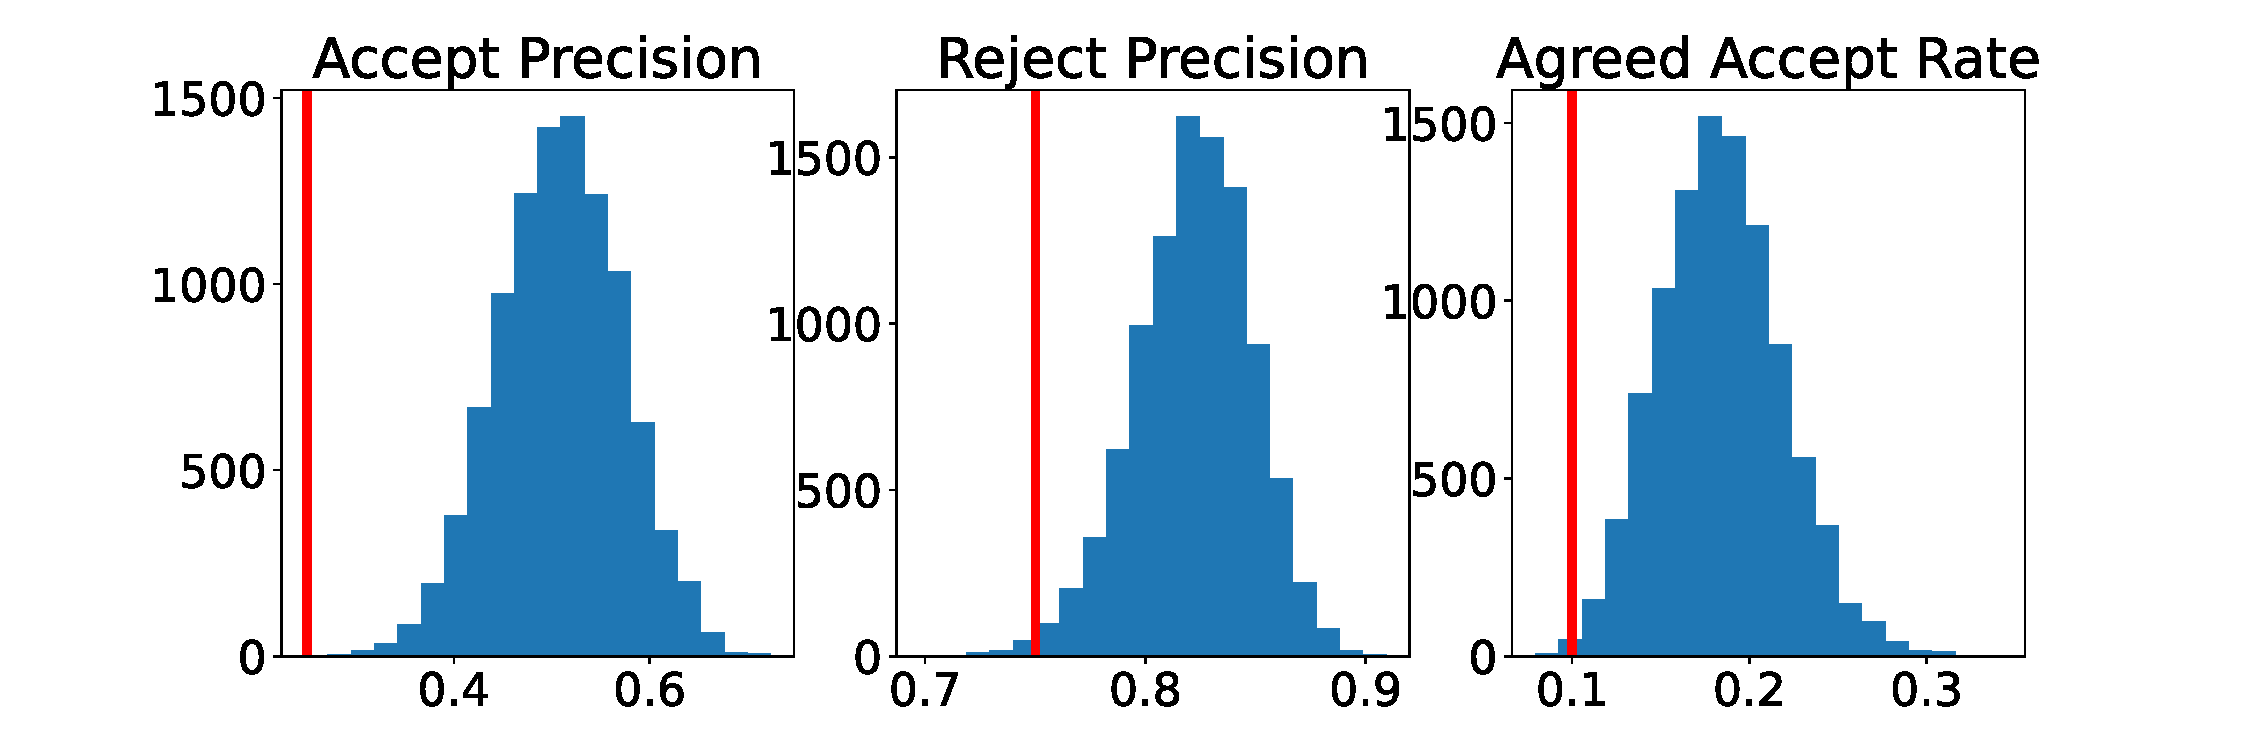
\includegraphics[width=0.90\textwidth]{diagrams/neurips/random-committee-outcomes-vs-true.pdf}


\caption{Different statistics for the random committee oucomes versus the observed committee outcomes.}
\label{random-committee-outcomes}
\end{figure}

\hypertarget{model-choice-and-prior-values}{%
\subsubsection{Model Choice and Prior
Values}\label{model-choice-and-prior-values}}

In the analysis above we've minimized the modeling choices: we made use
of a Bayesian analysis to capture the uncertainty in counts that can be
arising from statistical sampling error. To this end we chose an
uninformative prior over these probabilities. However, one might argue
that the prior should reflect something more about the underlying
experimental structure: for example we \emph{know} that if the
committees made their decisions independently it is unlikely that we'd
obtain an inconsistency figure much greater than 37.5\% because that
would require committees to explicitly collude to make inconsistent
decisions: the random conference is the worst case. Due to the accept
rate, we also expect a larger number of reject decisions than reject.
This also isn't captured in our prior. Such questions actually move us
into the realms of modeling the process, rather then performing a
sensitivity analysis. However, if we wish to model the decision process
as a whole we have a lot more information available, and we should make
use of it. The analysis above is intended to exploit our randomized
experiment to explore how inconsistent we expect two committees to be.
It focusses on that single question, it doesn't attempt to give answers
on what the reasons for that inconsistency are and how it may be
reduced. The additional maths was needed only to give a sense of the
uncertainty in the figures. That uncertainty arises due to the limited
number of papers in the experiment.

\hypertarget{reviewer-calibration}{%
\subsection{Reviewer Calibration}\label{reviewer-calibration}}

\begin{flushright}
[\href{https://github.com/lawrennd/talks/edit/gh-pages/_neurips/includes/neurips-reviewer-calibration.md}{edit}]
\end{flushright}

Calibration of reviewers is the process where different interpretations
of the reviewing scale are addressed. The tradition of calibration goes
at least as far back as John Platt's Program Chairing, and included a
Bayesian model by Ge, Welling and Ghahramani at NeurIPS 2013.

\hypertarget{reviewer-calibration-model}{%
\subsection{Reviewer Calibration
Model}\label{reviewer-calibration-model}}

\begin{flushright}
[\href{https://github.com/lawrennd/talks/edit/gh-pages/_neurips/includes/reviewer-calibration-model.md}{edit}]
\end{flushright}

In this note book we deal with reviewer calibration. Our assumption is
that the score from the \(j\)th reviwer for the \(i\)th paper is given
by \[
y_{i,j} = f_i + b_j + \epsilon_{i, j}
\] where \(f_i\) is the `objective quality' of paper \(i\) and \(b_j\)
is an offset associated with reviewer \(j\). \(\epsilon_{i,j}\) is a
subjective quality estimate which reflects how a specific reviewer's
opinion differs from other reviewers (such differences in opinion may be
due to differing expertise or perspective). The underlying `objective
quality' of the paper is assumed to be the same for all reviewers and
the reviewer offset is assumed to be the same for all papers.

If we have \(n\) papers and \(m\) reviewers then this implies \(n\) +
\(m\) + \(nm\) values need to be estimated. Naturally this is too many,
and we can start by assuming that the subjective quality is drawn from a
normal density with variance \(\sigma^2\) \[
\epsilon_{i, j} \sim N(0, \sigma^2 \mathbf{I})
\] which reduces us to \(n\) + \(m\) + 1 parameters. Further we can
assume that the objective quality is also normally distributed with mean
\(\mu\) and variance \(\alpha_f\), \[
f_i \sim N(\mu, \alpha_f)
\] this now reduces us to \(m\)+3 parameters. However, we only have
approximately \(4m\) observations (4 papers per reviewer) so parameters
may still not be that well determined (particularly for those reviewers
that have only one review). We therefore, finally, assume that reviewer
offset is normally distributed with zero mean, \[
b_j \sim N(0, \alpha_b),
\] leaving us only four parameters: \(\mu\), \(\sigma^2\), \(\alpha_f\)
and \(\alpha_b\). Combined together these three assumptions imply that
\[
\mathbf{y} \sim N(\mu \mathbf{1}, \mathbf{K})
\] where \(\mathbf{y}\) is a vector of stacked scores \(\mathbf{1}\) is
the vector of ones and the elements of the covariance function are given
by \[
k(i,j; k,l) = \delta_{i,k} \alpha_f + \delta_{j,l} \alpha_b + \delta_{i, k}\delta_{j,l} \sigma^2
\] where \(i\) and \(j\) are the index of first paper and reviewer and
\(k\) and \(l\) are the index of second paper and reviewer. The mean is
easily estimated by maximum likelihood, and is given as the mean of all
scores.

It is convenient to reparameterize slightly into an overall scale
\(\alpha_f\), and normalized variance parameters, \[
k(i,j; k,l) = \alpha_f(\delta_{i,k}  + \delta_{j,l} \frac{\alpha_b}{\alpha_f} + \delta_{i, k}\delta_{j,l} \frac{\sigma^2}{\alpha_f})
\] which we rewrite to give two ratios: offset/signal ratio,
\(\hat{\alpha}_b\) and noise/signal \(\hat{\sigma}^2\) ratio. \[
k(i,j; k,l) = \alpha_f(\delta_{i,k}  + \delta_{j,l} \hat{\alpha}_b + \delta_{i, k}\delta_{j,l} \hat{\sigma}^2)
\] The advantage of this parameterization is it allows us to optimize
\(\alpha_f\) directly (with a fixed point equation) and it will be very
well determined. This leaves us with two free parameters, that we can
explore on the grid. It is in these parameters that we expect the
remaining underdetermindness of the model. We expect \(\alpha_f\) to be
well determined because the negative log likelihood is now \[
\frac{|\mathbf{y}|}{2}\log\alpha_f + \frac{1}{2}\log  \left|\hat{\mathbf{K}}\right| + \frac{1}{2\alpha_f}\mathbf{y}^\top \hat{\mathbf{K}}^{-1} \mathbf{y}
\] where \(|\mathbf{y}|\) is the length of \(\mathbf{y}\) (i.e.~the
number of reviews) and \(\hat{\mathbf{K}}=\alpha_f^{-1}\mathbf{K}\) is
the scale normalised covariance. This negative log likelihood is easily
minimized to recover \[
\alpha_f = \frac{1}{|\mathbf{y}|} \mathbf{y}^\top \hat{\mathbf{K}}^{-1} \mathbf{y}
\] A Bayesian analysis of this parameter is possible with gamma priors,
but it would merely shows that this parameter is extremely well
determined (the degrees of freedom parameter of the associated
Student-\(t\) marginal likelihood scales will the number of reviews,
which will be around \(|\mathbf{y}| \approx 6,000\) in our case.

So, we propose to proceed as follows. Set the mean from the reviews
(\(\mu\)) and then choose a two dimensional grid of parameters for
reviewer offset and diversity. For each parameter choice, optimize to
find \(\alpha_f\) and then evaluate the liklihood. Worst case this will
require us inverting \(\hat{\mathbf{K}}\), but if the reviewer paper
groups are disconnected, it can be done a lot quicker. Next stage is to
load in the reviews for analysis.

\hypertarget{fitting-the-model}{%
\subsection{Fitting the Model}\label{fitting-the-model}}

\begin{flushright}
[\href{https://github.com/lawrennd/talks/edit/gh-pages/_neurips/includes/reviewer-calibration-fit-model.md}{edit}]
\end{flushright}

\begin{Shaded}
\begin{Highlighting}[]
\ImportTok{import}\NormalTok{ cmtutils }\ImportTok{as}\NormalTok{ cu}
\ImportTok{import}\NormalTok{ os}
\ImportTok{import}\NormalTok{ pandas }\ImportTok{as}\NormalTok{ pd}
\ImportTok{import}\NormalTok{ numpy }\ImportTok{as}\NormalTok{ np}
\ImportTok{import}\NormalTok{ GPy}
\ImportTok{from}\NormalTok{ scipy.sparse.csgraph }\ImportTok{import}\NormalTok{ connected\_components}
\ImportTok{from}\NormalTok{ scipy.linalg }\ImportTok{import}\NormalTok{ solve\_triangular }
\end{Highlighting}
\end{Shaded}

\begin{Shaded}
\begin{Highlighting}[]
\NormalTok{date }\OperatorTok{=} \StringTok{\textquotesingle{}2014{-}09{-}06\textquotesingle{}}
\end{Highlighting}
\end{Shaded}

\hypertarget{loading-in-the-data}{%
\subsection{Loading in the Data}\label{loading-in-the-data}}

\begin{Shaded}
\begin{Highlighting}[]
\NormalTok{filename }\OperatorTok{=}\NormalTok{ date }\OperatorTok{+} \StringTok{\textquotesingle{}\_reviews.xls\textquotesingle{}}
\NormalTok{reviews }\OperatorTok{=}\NormalTok{ cu.CMT\_Reviews\_read(filename}\OperatorTok{=}\NormalTok{filename)}
\NormalTok{papers }\OperatorTok{=} \BuiltInTok{list}\NormalTok{(}\BuiltInTok{sorted}\NormalTok{(}\BuiltInTok{set}\NormalTok{(reviews.reviews.index), key}\OperatorTok{=}\BuiltInTok{int}\NormalTok{))}
\NormalTok{reviews.reviews }\OperatorTok{=}\NormalTok{ reviews.reviews.loc[papers]}
\end{Highlighting}
\end{Shaded}

The maximum likelihood solution for \(\mu\) is simply the mean quality
of the papers, this is easily computed.

\begin{Shaded}
\begin{Highlighting}[]
\NormalTok{mu }\OperatorTok{=}\NormalTok{ reviews.reviews.Quality.mean()}
\BuiltInTok{print}\NormalTok{(}\StringTok{"Mean value, mu = "}\NormalTok{, mu)}
\end{Highlighting}
\end{Shaded}

\hypertarget{data-preparation}{%
\subsection{Data Preparation}\label{data-preparation}}

We take the reviews, which are indexed by the paper number, and create a
new data frame, that indexes by paper id and email combined. From these
reviews we tokenize the \texttt{PaperID} and the \texttt{Email} to
extract two matrices that can be used in creation of covariance
matrices. We also create a target vector which is the mean centred
vector of scores.

\begin{Shaded}
\begin{Highlighting}[]
\NormalTok{r }\OperatorTok{=}\NormalTok{ reviews.reviews.reset\_index()}
\NormalTok{r.rename(columns}\OperatorTok{=}\NormalTok{\{}\StringTok{\textquotesingle{}ID\textquotesingle{}}\NormalTok{:}\StringTok{\textquotesingle{}PaperID\textquotesingle{}}\NormalTok{\}, inplace}\OperatorTok{=}\VariableTok{True}\NormalTok{)}
\NormalTok{r.index }\OperatorTok{=}\NormalTok{ r.PaperID }\OperatorTok{+} \StringTok{\textquotesingle{}\_\textquotesingle{}} \OperatorTok{+}\NormalTok{ r.Email}
\NormalTok{X1 }\OperatorTok{=}\NormalTok{ pd.get\_dummies(r.PaperID)}
\NormalTok{X1 }\OperatorTok{=}\NormalTok{ X1[}\BuiltInTok{sorted}\NormalTok{(X1.columns, key}\OperatorTok{=}\BuiltInTok{int}\NormalTok{)]}
\NormalTok{X2 }\OperatorTok{=}\NormalTok{ pd.get\_dummies(r.Email)}
\NormalTok{X2 }\OperatorTok{=}\NormalTok{ X2[}\BuiltInTok{sorted}\NormalTok{(X2.columns, key}\OperatorTok{=}\BuiltInTok{str}\NormalTok{.lower)]}
\NormalTok{y }\OperatorTok{=}\NormalTok{ reviews.reviews.Quality }\OperatorTok{{-}}\NormalTok{ mu}
\end{Highlighting}
\end{Shaded}

\hypertarget{constructing-the-model-in-gpy}{%
\subsubsection{Constructing the Model in
GPy}\label{constructing-the-model-in-gpy}}

Having reduced the model to two parameters, I was hopeful I could set
parameters broadly by hand. My initial expectation was that
\texttt{alpha\_b} and \texttt{sigma2} would both be less than 1, but
some playing with parameters showed this wasn't the case. Rather than
waste further time, I decided to use our
\href{https://github.com/SheffieldML/GPy}{\texttt{GPy} Software} (see
below) to find a maximum likelihood solution for the parameters.

Model construction firstly involves constructing covariance functions
for the model and concatanating \texttt{X1} and \texttt{X2} to a new
input matrix \texttt{X}.

\begin{Shaded}
\begin{Highlighting}[]
\NormalTok{X }\OperatorTok{=}\NormalTok{ X1.join(X2)}
\NormalTok{kern1 }\OperatorTok{=}\NormalTok{ GPy.kern.Linear(input\_dim}\OperatorTok{=}\BuiltInTok{len}\NormalTok{(X1.columns), active\_dims}\OperatorTok{=}\NormalTok{np.arange(}\BuiltInTok{len}\NormalTok{(X1.columns)))}
\NormalTok{kern1.name }\OperatorTok{=} \StringTok{\textquotesingle{}K\_f\textquotesingle{}}
\NormalTok{kern2 }\OperatorTok{=}\NormalTok{ GPy.kern.Linear(input\_dim}\OperatorTok{=}\BuiltInTok{len}\NormalTok{(X2.columns), active\_dims}\OperatorTok{=}\NormalTok{np.arange(}\BuiltInTok{len}\NormalTok{(X1.columns), }\BuiltInTok{len}\NormalTok{(X.columns)))}
\NormalTok{kern2.name }\OperatorTok{=} \StringTok{\textquotesingle{}K\_b\textquotesingle{}}
\end{Highlighting}
\end{Shaded}

Next, the covariance function is used to create a Gaussian process
regression model with \texttt{X} as input and \texttt{y} as target. The
covariance function is given by \(\mathbf{K}_f + \mathbf{K}_b\).

\begin{Shaded}
\begin{Highlighting}[]
\NormalTok{model }\OperatorTok{=}\NormalTok{ GPy.models.GPRegression(X, y.to\_numpy()[:, np.newaxis], kern1}\OperatorTok{+}\NormalTok{kern2)}
\NormalTok{model.optimize()}
\end{Highlighting}
\end{Shaded}

Now we can check the parameters of the result.

\begin{Shaded}
\begin{Highlighting}[]
\BuiltInTok{print}\NormalTok{(model)}
\BuiltInTok{print}\NormalTok{(model.log\_likelihood())}
\end{Highlighting}
\end{Shaded}

\begin{verbatim}
    Name : GP regression
    Objective : 10071.679092815619
    Number of Parameters : 3
    Number of Optimization Parameters : 3
    Updates : True
    Parameters:
      GP_regression.           |               value  |  constraints  |  priors
      sum.K_f.variances        |  1.2782303448777643  |      +ve      |        
      sum.K_b.variances        |  0.2400098787580176  |      +ve      |        
      Gaussian_noise.variance  |  1.2683656892796749  |      +ve      |        
    -10071.679092815619
\end{verbatim}

\hypertarget{construct-the-model-without-gpy}{%
\subsubsection{Construct the Model Without
GPy}\label{construct-the-model-without-gpy}}

The answer from the GPy solution is introduced here, alongside the code
where the covariance matrices are explicitly created (above they are
created using GPy's high level code for kernel matrices, which may be
less clear on the details).

\begin{Shaded}
\begin{Highlighting}[]
\CommentTok{\# set parameter values to ML solutions given by GPy.}
\NormalTok{alpha\_f }\OperatorTok{=}\NormalTok{ model.}\BuiltInTok{sum}\NormalTok{.K\_f.variances}
\NormalTok{alpha\_b }\OperatorTok{=}\NormalTok{ model.}\BuiltInTok{sum}\NormalTok{.K\_b.variances}\OperatorTok{/}\NormalTok{alpha\_f}
\NormalTok{sigma2 }\OperatorTok{=}\NormalTok{ model.Gaussian\_noise.variance}\OperatorTok{/}\NormalTok{alpha\_f}
\end{Highlighting}
\end{Shaded}

Now we create the covariance functions based on the tokenized paper IDs
and emails.

\begin{Shaded}
\begin{Highlighting}[]
\NormalTok{K\_f }\OperatorTok{=}\NormalTok{ np.dot(X1, X1.T)}
\NormalTok{K\_b }\OperatorTok{=}\NormalTok{ alpha\_b}\OperatorTok{*}\NormalTok{np.dot(X2, X2.T)}
\NormalTok{K }\OperatorTok{=}\NormalTok{ K\_f }\OperatorTok{+}\NormalTok{ K\_b }\OperatorTok{+}\NormalTok{ sigma2}\OperatorTok{*}\NormalTok{np.eye(X2.shape[}\DecValTok{0}\NormalTok{])}
\NormalTok{Kinv, L, Li, logdet }\OperatorTok{=}\NormalTok{ GPy.util.linalg.pdinv(K) }\CommentTok{\# since we have GPy loaded in use their positive definite inverse.}
\NormalTok{y }\OperatorTok{=}\NormalTok{ reviews.reviews.Quality }\OperatorTok{{-}}\NormalTok{ mu}
\NormalTok{alpha }\OperatorTok{=}\NormalTok{ np.dot(Kinv, y)}
\NormalTok{yTKinvy }\OperatorTok{=}\NormalTok{ np.dot(y, alpha)}
\NormalTok{alpha\_f }\OperatorTok{=}\NormalTok{ yTKinvy}\OperatorTok{/}\BuiltInTok{len}\NormalTok{(y)}
\end{Highlighting}
\end{Shaded}

Since we have removed the data mean, the log likelihood we are
interested in is the likelihood of a multivariate Gaussian with
covariance \(\mathbf{K}\) and mean zero. This is computed below.

\begin{Shaded}
\begin{Highlighting}[]
\NormalTok{ll }\OperatorTok{=} \FloatTok{0.5}\OperatorTok{*}\BuiltInTok{len}\NormalTok{(y)}\OperatorTok{*}\NormalTok{np.log(}\DecValTok{2}\OperatorTok{*}\NormalTok{np.pi}\OperatorTok{*}\NormalTok{alpha\_f) }\OperatorTok{+} \FloatTok{0.5}\OperatorTok{*}\NormalTok{logdet }\OperatorTok{+} \FloatTok{0.5}\OperatorTok{*}\NormalTok{yTKinvy}\OperatorTok{/}\NormalTok{alpha\_f }
\BuiltInTok{print}\NormalTok{(}\StringTok{"negative log likelihood: "}\NormalTok{, ll)}
\end{Highlighting}
\end{Shaded}

\hypertarget{review-quality-prediction}{%
\subsubsection{Review Quality
Prediction}\label{review-quality-prediction}}

\begin{flushright}
[\href{https://github.com/lawrennd/talks/edit/gh-pages/_neurips/includes/review-quality-prediction.md}{edit}]
\end{flushright}

Now we wish to predict the bias corrected scores for the papers. That
involves considering a variable \(s_{i,j} = f_i + e_{i,j}\) which is the
score with the bias removed. That variable has a covariance matrix,
\(\mathbf{K}_s=\mathbf{K}_f + \sigma^2 \mathbf{I}\) and a cross
covariance between \(\mathbf{y}\) and \(\mathbf{s}\) is also given by
\(\mathbf{K}_s\). This means we can compute the posterior distribution
of the scores as follows:

\begin{Shaded}
\begin{Highlighting}[]
\CommentTok{\# Compute mean and covariance of quality scores}
\NormalTok{K\_s }\OperatorTok{=}\NormalTok{ K\_f }\OperatorTok{+}\NormalTok{ np.eye(K\_f.shape[}\DecValTok{0}\NormalTok{])}\OperatorTok{*}\NormalTok{sigma2}
\NormalTok{s }\OperatorTok{=}\NormalTok{ pd.Series(np.dot(K\_s, alpha) }\OperatorTok{+}\NormalTok{ mu, index}\OperatorTok{=}\NormalTok{X1.index)}
\NormalTok{covs }\OperatorTok{=}\NormalTok{ alpha\_f}\OperatorTok{*}\NormalTok{(K\_s }\OperatorTok{{-}}\NormalTok{ np.dot(K\_s, np.dot(Kinv, K\_s)))}
\end{Highlighting}
\end{Shaded}

\hypertarget{monte-carlo-simulations-for-probability-of-acceptance}{%
\subsubsection{Monte Carlo Simulations for Probability of
Acceptance}\label{monte-carlo-simulations-for-probability-of-acceptance}}

\begin{flushright}
[\href{https://github.com/lawrennd/talks/edit/gh-pages/_neurips/includes/paper-acceptance-monte-carlo.md}{edit}]
\end{flushright}

We can now sample from this posterior distribution of bias-adjusted
scores jointly, to get a set of scores for all papers. For this set of
scores we can perform a ranking and accept the top 400 papers. This
gives us a sampled conference. If we do that 1,000 times then we can see
how many times each paper was accepted to get a probability of
acceptance.

\begin{Shaded}
\begin{Highlighting}[]
\NormalTok{number\_accepts }\OperatorTok{=} \DecValTok{420} \CommentTok{\# 440 because of the 10\% replication}
\end{Highlighting}
\end{Shaded}

\begin{Shaded}
\begin{Highlighting}[]
\CommentTok{\# place this in a separate box, because sampling can take a while.}
\NormalTok{samples }\OperatorTok{=} \DecValTok{1000}
\NormalTok{score }\OperatorTok{=}\NormalTok{ np.random.multivariate\_normal(mean}\OperatorTok{=}\NormalTok{s, cov}\OperatorTok{=}\NormalTok{covs, size}\OperatorTok{=}\NormalTok{samples).T}
\CommentTok{\# Use X1 which maps papers to paper/reviewer pairings to get the average score for each paper.}
\NormalTok{paper\_score }\OperatorTok{=}\NormalTok{ pd.DataFrame(np.dot(np.diag(}\FloatTok{1.}\OperatorTok{/}\NormalTok{X1.}\BuiltInTok{sum}\NormalTok{(}\DecValTok{0}\NormalTok{)), np.dot(X1.T, score)), index}\OperatorTok{=}\NormalTok{X1.columns)}
\end{Highlighting}
\end{Shaded}

Now we can compute the probability of acceptance for each of the sampled
rankings.

\begin{Shaded}
\begin{Highlighting}[]
\NormalTok{prob\_accept }\OperatorTok{=}\NormalTok{ ((paper\_score}\OperatorTok{\textgreater{}}\NormalTok{paper\_score.quantile(}\DecValTok{1}\OperatorTok{{-}}\NormalTok{(}\BuiltInTok{float}\NormalTok{(number\_accepts)}\OperatorTok{/}\NormalTok{paper\_score.shape[}\DecValTok{0}\NormalTok{]))).}\BuiltInTok{sum}\NormalTok{(}\DecValTok{1}\NormalTok{)}\OperatorTok{/}\DecValTok{1000}\NormalTok{)}
\NormalTok{prob\_accept.name }\OperatorTok{=} \StringTok{\textquotesingle{}AcceptProbability\textquotesingle{}}
\end{Highlighting}
\end{Shaded}

Now we have the probability of accepts, we can decide on the boundaries
of the grey area. These are set in \texttt{lower} and \texttt{upper}.
The grey area is those papers that will be debated most heavily during
the teleconferences between program chairs and area chairs.

\begin{Shaded}
\begin{Highlighting}[]
\NormalTok{lower}\OperatorTok{=}\FloatTok{0.1}
\NormalTok{upper}\OperatorTok{=}\FloatTok{0.9}
\NormalTok{grey\_area }\OperatorTok{=}\NormalTok{ ((prob\_accept}\OperatorTok{\textgreater{}}\NormalTok{lower) }\OperatorTok{\&}\NormalTok{ (prob\_accept}\OperatorTok{\textless{}}\NormalTok{upper))}
\BuiltInTok{print}\NormalTok{(}\StringTok{\textquotesingle{}Number of papers in grey area:\textquotesingle{}}\NormalTok{, grey\_area.}\BuiltInTok{sum}\NormalTok{())}
\end{Highlighting}
\end{Shaded}

\begin{Shaded}
\begin{Highlighting}[]
\ImportTok{import}\NormalTok{ matplotlib.pyplot }\ImportTok{as}\NormalTok{ plt}
\ImportTok{import}\NormalTok{ cmtutils.plot }\ImportTok{as}\NormalTok{ plot}
\end{Highlighting}
\end{Shaded}

\begin{Shaded}
\begin{Highlighting}[]
\NormalTok{fig, ax }\OperatorTok{=}\NormalTok{ plt.subplots(figsize}\OperatorTok{=}\NormalTok{plot.big\_wide\_figsize)}
\BuiltInTok{print}\NormalTok{(}\StringTok{\textquotesingle{}Expected Papers Accepted:\textquotesingle{}}\NormalTok{, prob\_accept.}\BuiltInTok{sum}\NormalTok{())}
\NormalTok{\_ }\OperatorTok{=}\NormalTok{ prob\_accept.hist(bins}\OperatorTok{=}\DecValTok{40}\NormalTok{, ax}\OperatorTok{=}\NormalTok{ax)}
\NormalTok{ma.write\_figure(directory}\OperatorTok{=}\StringTok{"./neurips"}\NormalTok{, filename}\OperatorTok{=}\StringTok{"probability{-}of{-}accept.svg"}\NormalTok{)}
\end{Highlighting}
\end{Shaded}

\begin{figure}[htb]
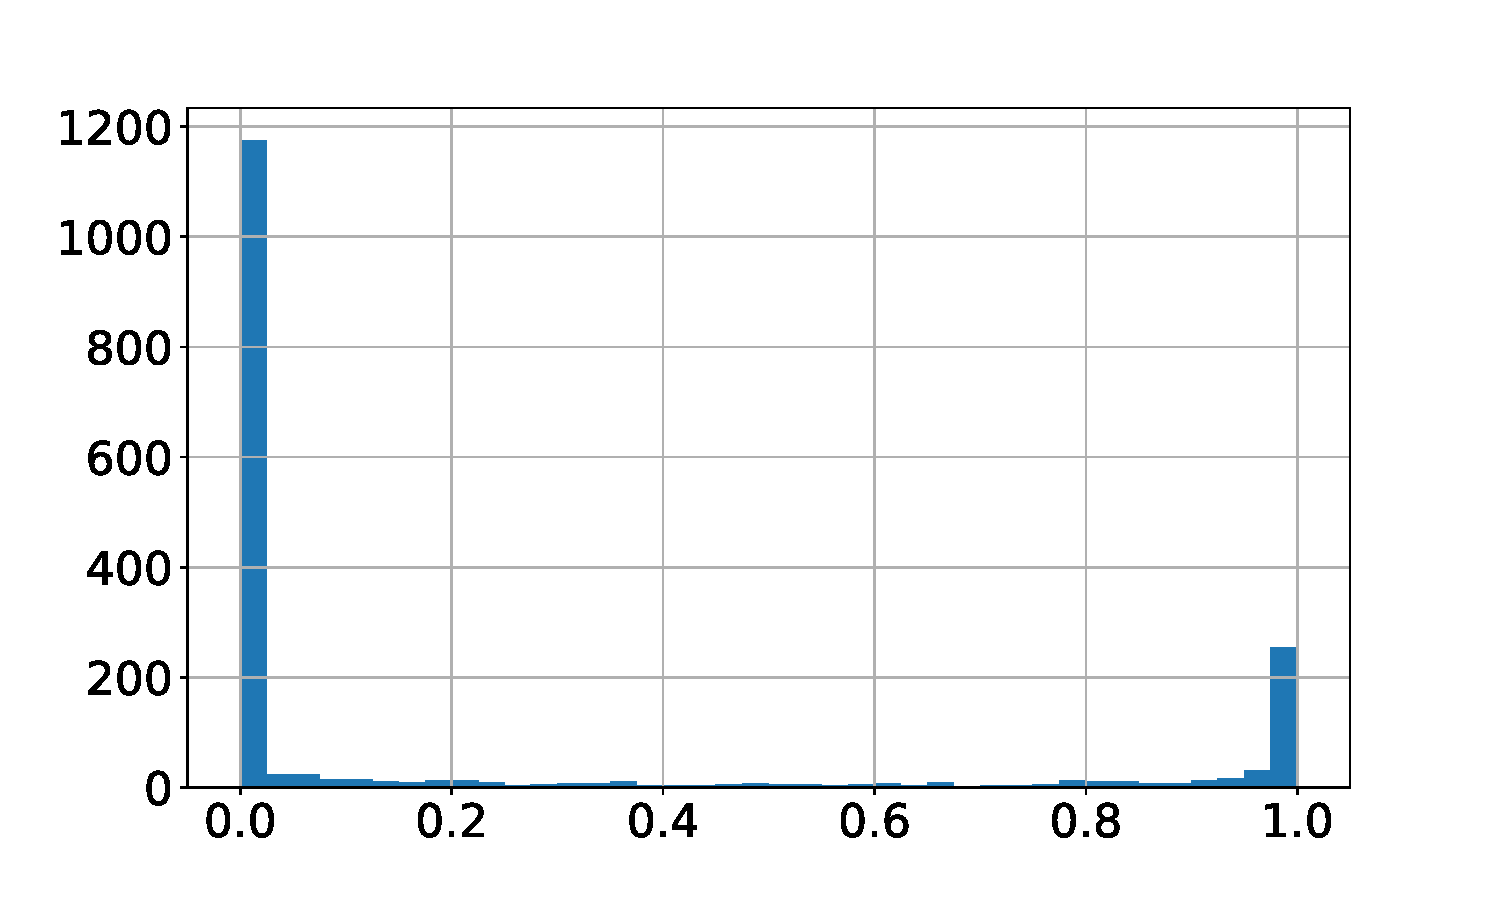
\includegraphics[width=0.70\textwidth]{diagrams/neurips/probability-of-accept.pdf}


\caption{Histogram of the probability of accept as estimated by the Monte Carlo simulation across all papers submitted to NeurIPS 2014.}
\label{probability-of-accept}
\end{figure}

\hypertarget{some-sanity-histograms}{%
\subsection{Some Sanity Histograms}\label{some-sanity-histograms}}

\begin{flushright}
[\href{https://github.com/lawrennd/talks/edit/gh-pages/_neurips/includes/calibration-sanity-checks.md}{edit}]
\end{flushright}

Here is the histogram of the reviewer scores after calibration.

\begin{Shaded}
\begin{Highlighting}[]
\NormalTok{fig, ax }\OperatorTok{=}\NormalTok{ plt.subplots(figsize}\OperatorTok{=}\NormalTok{plot.big\_wide\_figsize)}
\NormalTok{s.hist(bins}\OperatorTok{=}\DecValTok{100}\NormalTok{, ax}\OperatorTok{=}\NormalTok{ax)}
\NormalTok{\_ }\OperatorTok{=}\NormalTok{ ax.set\_title(}\StringTok{\textquotesingle{}Calibrated Reviewer Scores\textquotesingle{}}\NormalTok{)}
\NormalTok{ma.write\_figure(directory}\OperatorTok{=}\StringTok{"./neurips"}\NormalTok{, filename}\OperatorTok{=}\StringTok{"calibrated{-}reviewer{-}scores.svg"}\NormalTok{)}
\end{Highlighting}
\end{Shaded}

\begin{figure}[htb]
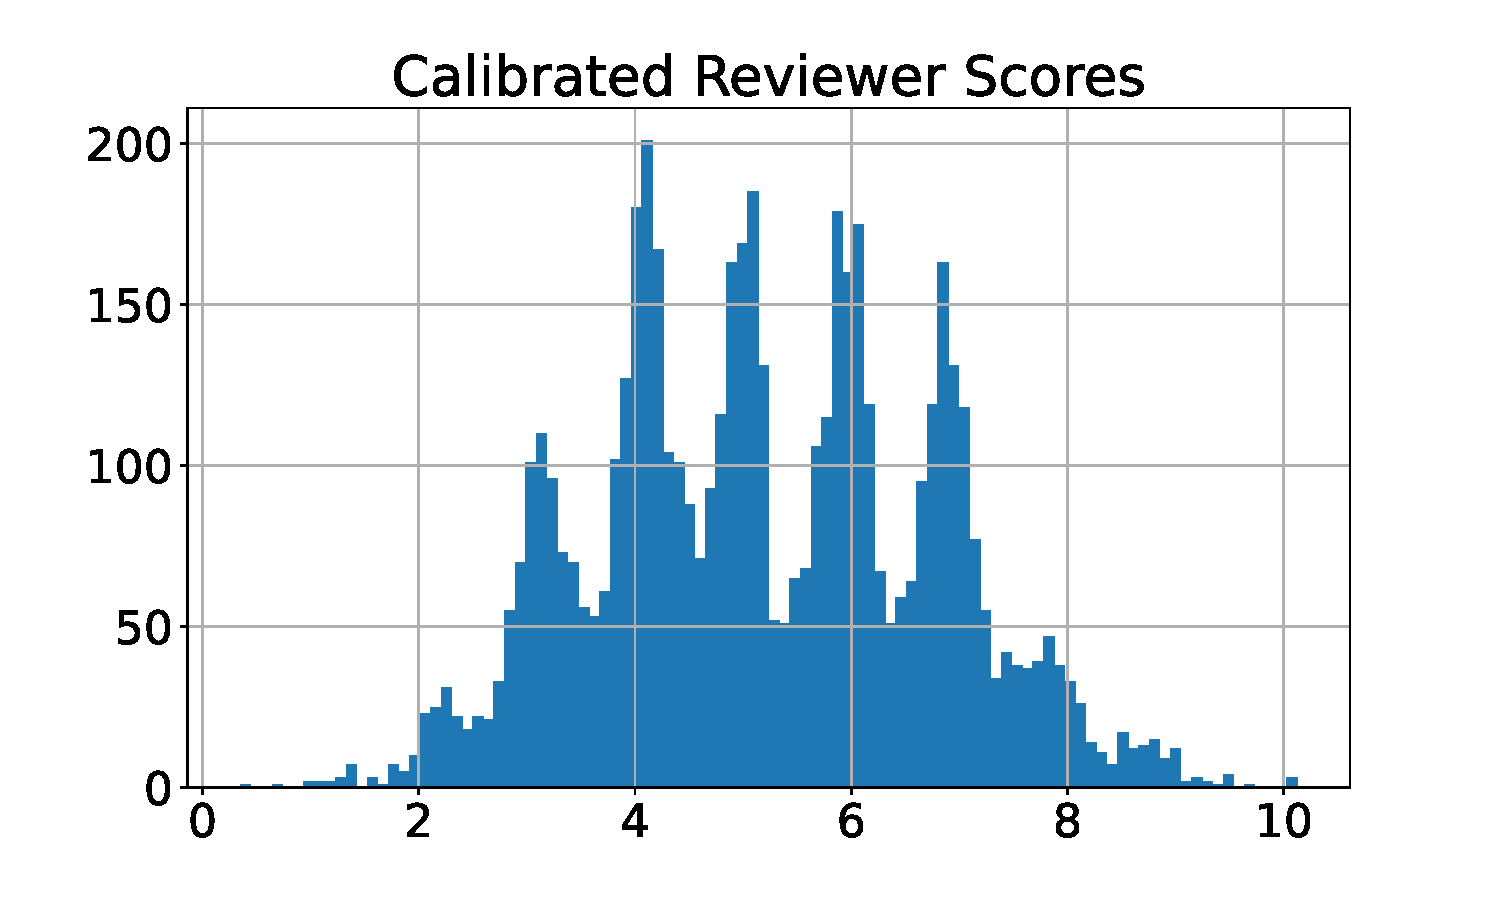
\includegraphics[width=0.70\textwidth]{diagrams/neurips/calibrated-reviewer-scores.pdf}


\caption{Histogram of updated reviewer scores after the calibration process is applied.}
\label{calibrated-reviewer-scores}
\end{figure}

\hypertarget{adjustments-to-reviewer-scores}{%
\subsubsection{Adjustments to Reviewer
Scores}\label{adjustments-to-reviewer-scores}}

We can also compute the posterior distribution for the adjustments to
the reviewer scores.

\begin{Shaded}
\begin{Highlighting}[]
\CommentTok{\# Compute mean and covariance of review biases}
\NormalTok{b }\OperatorTok{=}\NormalTok{ pd.Series(np.dot(K\_b, alpha), index}\OperatorTok{=}\NormalTok{X2.index)}
\NormalTok{covb }\OperatorTok{=}\NormalTok{ alpha\_f}\OperatorTok{*}\NormalTok{(K\_b }\OperatorTok{{-}}\NormalTok{ np.dot(K\_b, np.dot(Kinv, K\_b)))}
\end{Highlighting}
\end{Shaded}

\begin{Shaded}
\begin{Highlighting}[]
\NormalTok{reviewer\_bias }\OperatorTok{=}\NormalTok{ pd.Series(np.dot(np.diag(}\FloatTok{1.}\OperatorTok{/}\NormalTok{X2.}\BuiltInTok{sum}\NormalTok{(}\DecValTok{0}\NormalTok{)), np.dot(X2.T, b)), index}\OperatorTok{=}\NormalTok{X2.columns, name}\OperatorTok{=}\StringTok{\textquotesingle{}ReviewerBiasMean\textquotesingle{}}\NormalTok{)}
\NormalTok{reviewer\_bias\_std }\OperatorTok{=}\NormalTok{ pd.Series(np.dot(np.diag(}\FloatTok{1.}\OperatorTok{/}\NormalTok{X2.}\BuiltInTok{sum}\NormalTok{(}\DecValTok{0}\NormalTok{)), np.dot(X2.T, np.sqrt(np.diag(covb)))), index}\OperatorTok{=}\NormalTok{X2.columns, name}\OperatorTok{=}\StringTok{\textquotesingle{}ReviewerBiasStd\textquotesingle{}}\NormalTok{)}
\end{Highlighting}
\end{Shaded}

Here is a histogram of the mean adjustment for the reviewers.

\begin{Shaded}
\begin{Highlighting}[]
\NormalTok{fig, ax }\OperatorTok{=}\NormalTok{ plt.subplots(figsize}\OperatorTok{=}\NormalTok{plot.big\_wide\_figsize)}
\NormalTok{reviewer\_bias.hist(bins}\OperatorTok{=}\DecValTok{100}\NormalTok{, ax}\OperatorTok{=}\NormalTok{ax)}
\NormalTok{\_ }\OperatorTok{=}\NormalTok{ ax.set\_title(}\StringTok{\textquotesingle{}Reviewer Calibration Adjustments Histogram\textquotesingle{}}\NormalTok{)}
\NormalTok{ma.write\_figure(directory}\OperatorTok{=}\StringTok{"./neurips"}\NormalTok{, filename}\OperatorTok{=}\StringTok{"reviewer{-}calibration{-}adjustments.svg"}\NormalTok{)}
\end{Highlighting}
\end{Shaded}

\begin{figure}[htb]
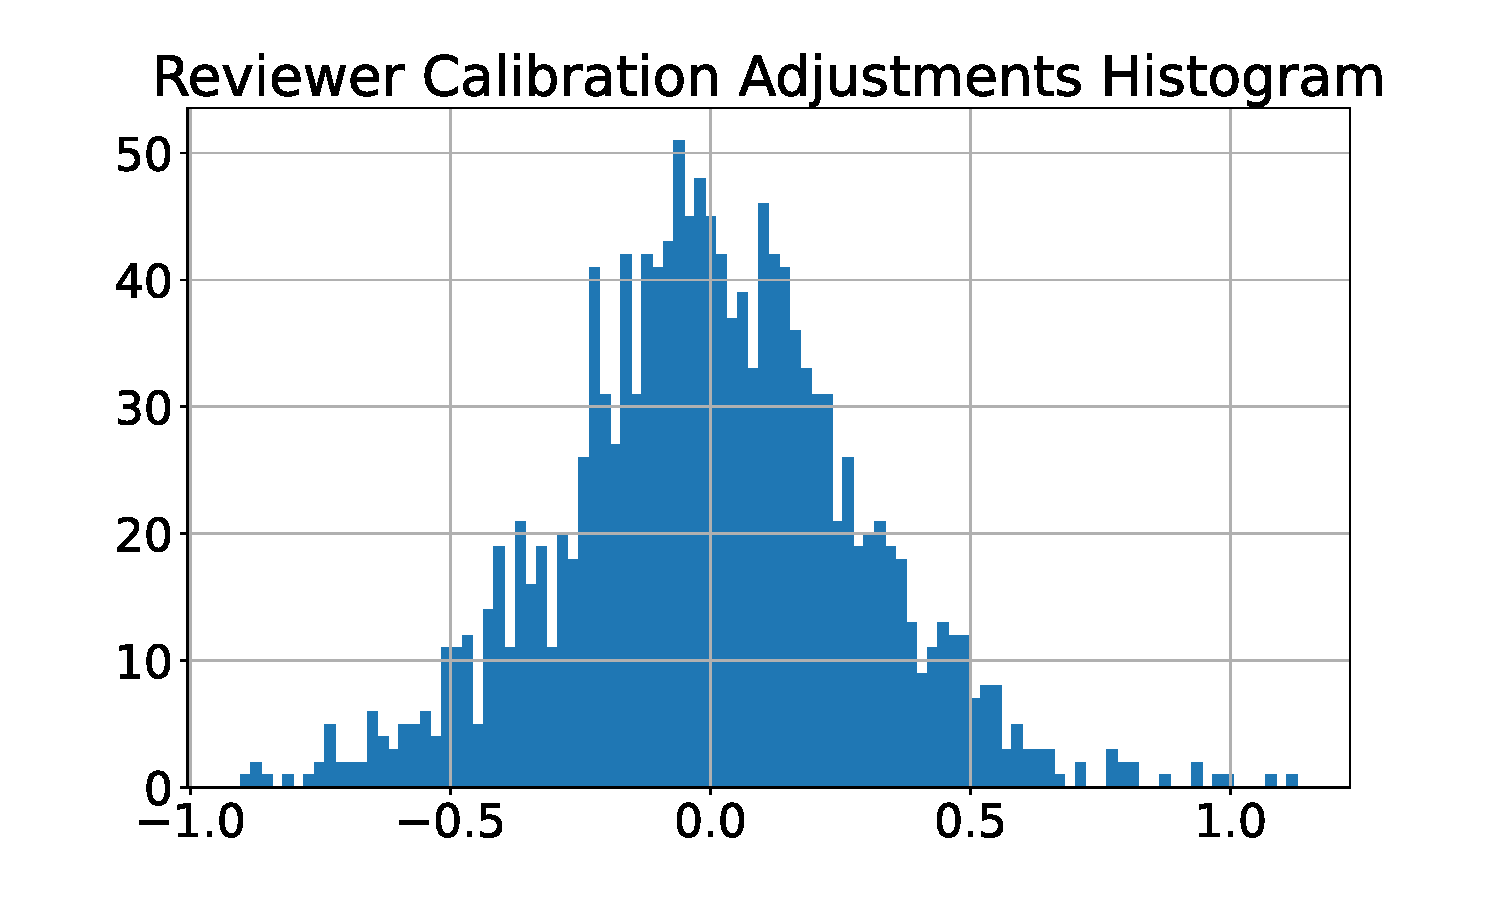
\includegraphics[width=0.70\textwidth]{diagrams/neurips/reviewer-calibration-adjustments.pdf}


\caption{Histogram of individual offsets associated with the reviewers as estimated by the model.}
\label{reviewer-calibration-adjustments}
\end{figure}

Export a version of the bias scores for use in CMT.

\begin{Shaded}
\begin{Highlighting}[]
\NormalTok{bias\_export }\OperatorTok{=}\NormalTok{ pd.DataFrame(data}\OperatorTok{=}\NormalTok{\{}\StringTok{\textquotesingle{}Quality Score {-} Does the paper deserves to be published?\textquotesingle{}}\NormalTok{:reviewer\_bias, }
                   \StringTok{\textquotesingle{}Impact Score {-} Independently of the Quality Score above, this is your opportunity to identify papers that are very different, original, or otherwise potentially impactful for the NIPS community.\textquotesingle{}}\NormalTok{:pd.Series(np.zeros(}\BuiltInTok{len}\NormalTok{(reviewer\_bias)), index}\OperatorTok{=}\NormalTok{reviewer\_bias.index),}
                    \StringTok{\textquotesingle{}Confidence\textquotesingle{}}\NormalTok{:pd.Series(np.zeros(}\BuiltInTok{len}\NormalTok{(reviewer\_bias)), index}\OperatorTok{=}\NormalTok{reviewer\_bias.index)\})}
\NormalTok{cols }\OperatorTok{=}\NormalTok{ bias\_export.columns.tolist()}
\NormalTok{cols }\OperatorTok{=}\NormalTok{ [cols[}\DecValTok{2}\NormalTok{], cols[}\DecValTok{1}\NormalTok{], cols[}\DecValTok{0}\NormalTok{]]}
\NormalTok{bias\_export }\OperatorTok{=}\NormalTok{ bias\_export[cols]}
\CommentTok{\#bias\_export.to\_csv(os.path.join(cu.cmt\_data\_directory, \textquotesingle{}reviewer\_bias.csv\textquotesingle{}), sep=\textquotesingle{}\textbackslash{}t\textquotesingle{}, header=True, index\_label=\textquotesingle{}Reviewer Email\textquotesingle{})}
\end{Highlighting}
\end{Shaded}

\hypertarget{sanity-check}{%
\subsection{Sanity Check}\label{sanity-check}}

As a sanity check Corinna suggested it makes sense to plot the average
raw score for the papers vs the probability of accept, just to ensure
nothing weird is going on. To clarify the plot, I've actually plotted
raw score vs log odds of accept.

\begin{Shaded}
\begin{Highlighting}[]
\NormalTok{raw\_score }\OperatorTok{=}\NormalTok{ pd.Series(np.dot(np.diag(}\FloatTok{1.}\OperatorTok{/}\NormalTok{X1.}\BuiltInTok{sum}\NormalTok{(}\DecValTok{0}\NormalTok{)), np.dot(X1.T, r.Quality)), index}\OperatorTok{=}\NormalTok{X1.columns)}
\NormalTok{prob\_accept[prob\_accept}\OperatorTok{==}\DecValTok{0}\NormalTok{] }\OperatorTok{=} \DecValTok{1}\OperatorTok{/}\NormalTok{(}\DecValTok{10}\OperatorTok{*}\NormalTok{samples)}
\NormalTok{prob\_accept[prob\_accept}\OperatorTok{==}\DecValTok{1}\NormalTok{] }\OperatorTok{=} \DecValTok{1}\OperatorTok{{-}}\DecValTok{1}\OperatorTok{/}\NormalTok{(}\DecValTok{10}\OperatorTok{*}\NormalTok{samples)}
\end{Highlighting}
\end{Shaded}

\begin{Shaded}
\begin{Highlighting}[]
\NormalTok{fig, ax }\OperatorTok{=}\NormalTok{ plt.subplots(figsize}\OperatorTok{=}\NormalTok{plot.big\_wide\_figsize)}
\NormalTok{ax.plot(raw\_score, np.log(prob\_accept)}\OperatorTok{{-}}\NormalTok{ np.log(}\DecValTok{1}\OperatorTok{{-}}\NormalTok{prob\_accept), }\StringTok{\textquotesingle{}rx\textquotesingle{}}\NormalTok{)}
\NormalTok{ax.set\_title(}\StringTok{\textquotesingle{}Raw Score vs Log odds of accept\textquotesingle{}}\NormalTok{)}
\NormalTok{ax.set\_xlabel(}\StringTok{\textquotesingle{}raw score\textquotesingle{}}\NormalTok{)}
\NormalTok{\_ }\OperatorTok{=}\NormalTok{ ax.set\_ylabel(}\StringTok{\textquotesingle{}log odds of accept\textquotesingle{}}\NormalTok{)}
\NormalTok{ma.write\_figure(directory}\OperatorTok{=}\StringTok{"./neurips"}\NormalTok{, filename}\OperatorTok{=}\StringTok{"raw{-}score{-}vs{-}log{-}odds.svg"}\NormalTok{)}
\end{Highlighting}
\end{Shaded}

\begin{figure}[htb]
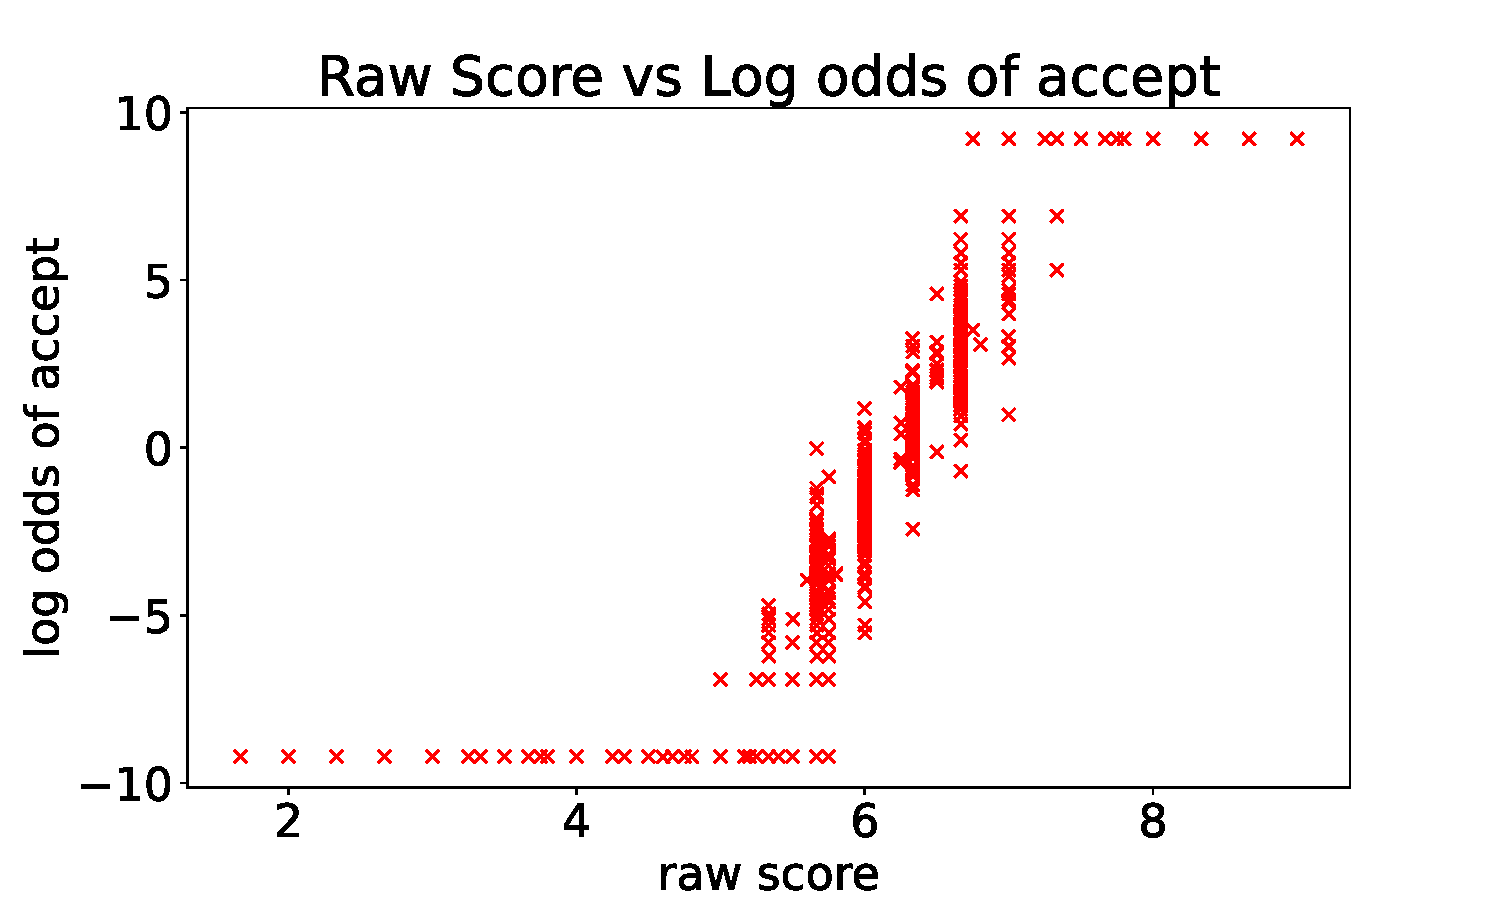
\includegraphics[width=0.70\textwidth]{diagrams/neurips/raw-score-vs-log-odds.pdf}


\caption{Histogram of the raw paper score against the log probability of paper acceptance, as estimated by Monte Carlo simulation.}
\label{raw-score-vs-log-odds}
\end{figure}

\hypertarget{calibraton-quality-sanity-checks}{%
\subsection{Calibraton Quality Sanity
Checks}\label{calibraton-quality-sanity-checks}}

\begin{Shaded}
\begin{Highlighting}[]
\NormalTok{s.name }\OperatorTok{=} \StringTok{\textquotesingle{}CalibratedQuality\textquotesingle{}}
\NormalTok{r }\OperatorTok{=}\NormalTok{ r.join(s)}
\end{Highlighting}
\end{Shaded}

We can also look at a scatter plot of the review quality vs the
calibrated quality.

\begin{Shaded}
\begin{Highlighting}[]
\NormalTok{fig, ax }\OperatorTok{=}\NormalTok{ plt.subplots(figsize}\OperatorTok{=}\NormalTok{plot.big\_wide\_figsize)}
\NormalTok{ax.plot(r.Quality, r.CalibratedQuality, }\StringTok{\textquotesingle{}r.\textquotesingle{}}\NormalTok{, markersize}\OperatorTok{=}\DecValTok{10}\NormalTok{)}
\NormalTok{ax.set\_xlim([}\DecValTok{0}\NormalTok{, }\DecValTok{11}\NormalTok{])}
\NormalTok{ax.set\_xlabel(}\StringTok{\textquotesingle{}original review score\textquotesingle{}}\NormalTok{)}
\NormalTok{\_ }\OperatorTok{=}\NormalTok{ ax.set\_ylabel(}\StringTok{\textquotesingle{}calibrated review score\textquotesingle{}}\NormalTok{)}
\NormalTok{ma.write\_figure(directory}\OperatorTok{=}\StringTok{"./neurips"}\NormalTok{, filename}\OperatorTok{=}\StringTok{"calibrated{-}review{-}score{-}vs{-}original{-}score.svg"}\NormalTok{)}
\end{Highlighting}
\end{Shaded}

\begin{figure}[htb]
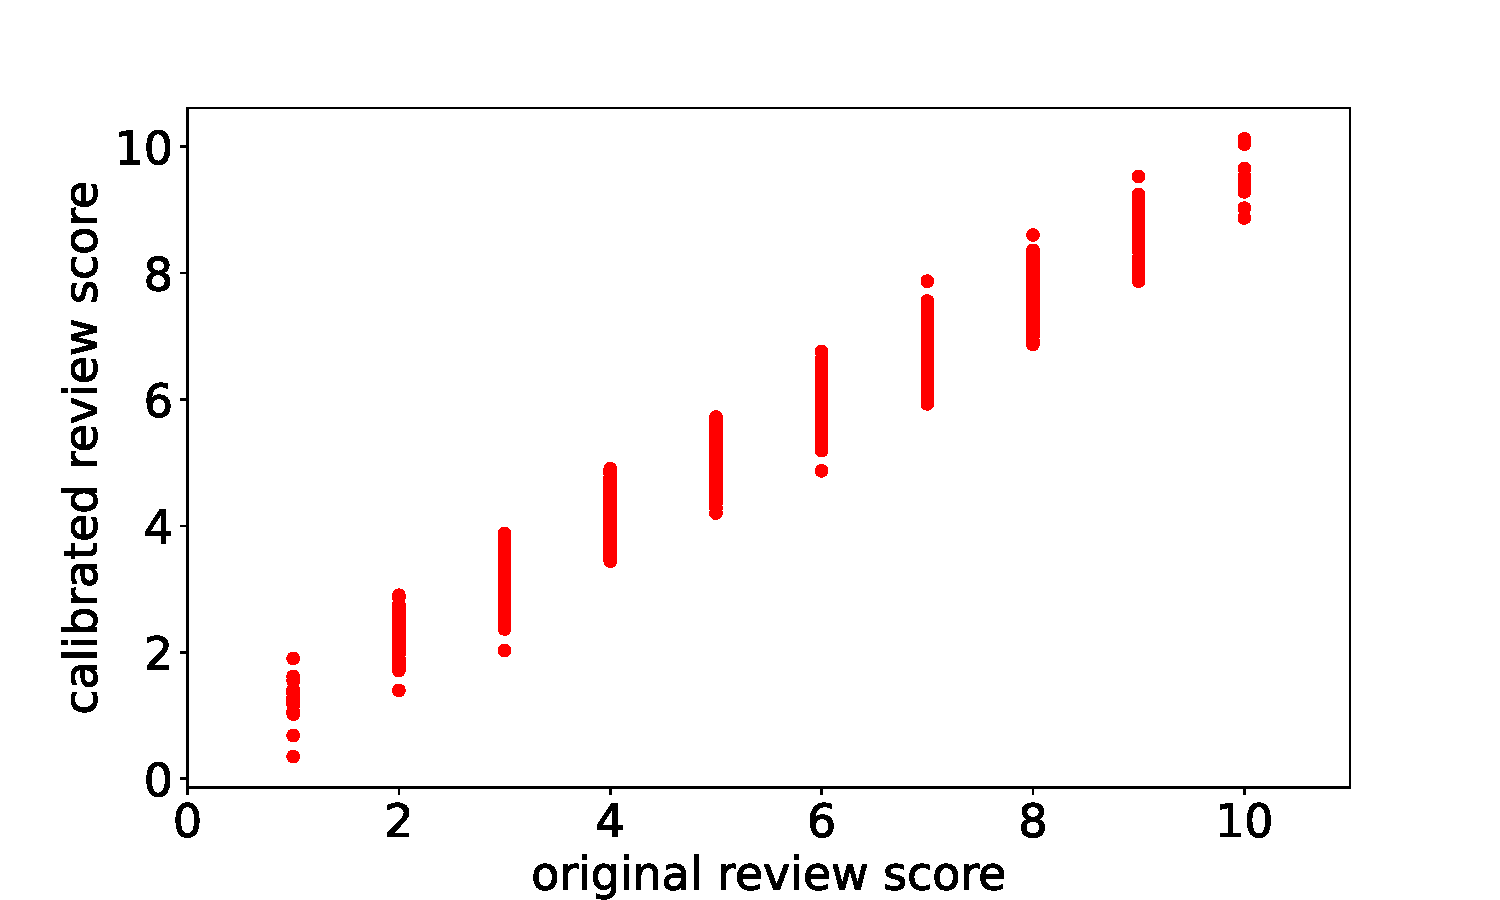
\includegraphics[width=0.70\textwidth]{diagrams/neurips/calibrated-review-score-vs-original-score.pdf}


\caption{Scatter plot of the calibrated review scores against the original review scores.}
\label{calibrated-review-vs-original-score}
\end{figure}

\hypertarget{correlation-of-duplicate-papers}{%
\subsection{Correlation of Duplicate
Papers}\label{correlation-of-duplicate-papers}}

\begin{flushright}
[\href{https://github.com/lawrennd/talks/edit/gh-pages/_neurips/includes/calibration-correlation-of-duplicate-papers.md}{edit}]
\end{flushright}

For NeurIPS 2014 we experimented with duplicate papers: we pushed papers
through the system twice, exposing them to different subsets of the
reviewers. The first thing we'll look at is the duplicate papers.
Firstly we identify them by matching on title.

\begin{Shaded}
\begin{Highlighting}[]
\NormalTok{filename }\OperatorTok{=}\NormalTok{ date }\OperatorTok{+} \StringTok{\textquotesingle{}\_paper\_list.xls\textquotesingle{}}
\NormalTok{papers }\OperatorTok{=}\NormalTok{ cu.CMT\_Papers\_read(filename}\OperatorTok{=}\NormalTok{filename)}
\NormalTok{duplicate\_list }\OperatorTok{=}\NormalTok{ []}
\ControlFlowTok{for}\NormalTok{ ID, title }\KeywordTok{in}\NormalTok{ papers.papers.Title.iteritems():}
    \ControlFlowTok{if} \BuiltInTok{int}\NormalTok{(ID)}\OperatorTok{\textgreater{}}\DecValTok{1779} \KeywordTok{and} \BuiltInTok{int}\NormalTok{(ID) }\OperatorTok{!=} \DecValTok{1949}\NormalTok{:}
\NormalTok{        pair }\OperatorTok{=} \BuiltInTok{list}\NormalTok{(papers.papers[papers.papers[}\StringTok{\textquotesingle{}Title\textquotesingle{}}\NormalTok{].}\BuiltInTok{str}\NormalTok{.contains(papers.papers.Title[ID].strip())].index)}
\NormalTok{        pair.sort(key}\OperatorTok{=}\BuiltInTok{int}\NormalTok{)}
\NormalTok{        duplicate\_list.append(pair)}
\end{Highlighting}
\end{Shaded}

Next we compute the correlation coefficients for the duplicated papers
for the average impact and quality scores.

\begin{Shaded}
\begin{Highlighting}[]
\NormalTok{quality }\OperatorTok{=}\NormalTok{ []}
\NormalTok{calibrated\_quality }\OperatorTok{=}\NormalTok{ []}
\NormalTok{accept }\OperatorTok{=}\NormalTok{ []}
\NormalTok{impact }\OperatorTok{=}\NormalTok{ []}
\NormalTok{confidence }\OperatorTok{=}\NormalTok{ []}
\ControlFlowTok{for}\NormalTok{ duplicate\_pair }\KeywordTok{in}\NormalTok{ duplicate\_list:}
\NormalTok{    quality.append([np.mean(r[r.PaperID}\OperatorTok{==}\NormalTok{duplicate\_pair[}\DecValTok{0}\NormalTok{]].Quality), np.mean(r[r.PaperID}\OperatorTok{==}\NormalTok{duplicate\_pair[}\DecValTok{1}\NormalTok{]].Quality)])}
\NormalTok{    calibrated\_quality.append([np.mean(r[r.PaperID}\OperatorTok{==}\NormalTok{duplicate\_pair[}\DecValTok{0}\NormalTok{]].CalibratedQuality), np.mean(r[r.PaperID}\OperatorTok{==}\NormalTok{duplicate\_pair[}\DecValTok{1}\NormalTok{]].CalibratedQuality)])}
\NormalTok{    impact.append([np.mean(r[r.PaperID}\OperatorTok{==}\NormalTok{duplicate\_pair[}\DecValTok{0}\NormalTok{]].Impact), np.mean(r[r.PaperID}\OperatorTok{==}\NormalTok{duplicate\_pair[}\DecValTok{1}\NormalTok{]].Impact)])}
\NormalTok{    confidence.append([np.mean(r[r.PaperID}\OperatorTok{==}\NormalTok{duplicate\_pair[}\DecValTok{0}\NormalTok{]].Conf), np.mean(r[r.PaperID}\OperatorTok{==}\NormalTok{duplicate\_pair[}\DecValTok{1}\NormalTok{]].Conf)])}
\NormalTok{quality }\OperatorTok{=}\NormalTok{ np.array(quality)}
\NormalTok{calibrated\_quality }\OperatorTok{=}\NormalTok{ np.array(calibrated\_quality)}
\NormalTok{impact }\OperatorTok{=}\NormalTok{ np.array(impact)}
\NormalTok{confidence }\OperatorTok{=}\NormalTok{ np.array(confidence)}
\NormalTok{quality\_cor }\OperatorTok{=}\NormalTok{ np.corrcoef(quality.T)[}\DecValTok{0}\NormalTok{, }\DecValTok{1}\NormalTok{]}
\NormalTok{calibrated\_quality\_cor }\OperatorTok{=}\NormalTok{ np.corrcoef(calibrated\_quality.T)[}\DecValTok{0}\NormalTok{, }\DecValTok{1}\NormalTok{]}
\NormalTok{impact\_cor }\OperatorTok{=}\NormalTok{ np.corrcoef(impact.T)[}\DecValTok{0}\NormalTok{, }\DecValTok{1}\NormalTok{]}
\NormalTok{confidence\_cor }\OperatorTok{=}\NormalTok{ np.corrcoef(confidence.T)[}\DecValTok{0}\NormalTok{, }\DecValTok{1}\NormalTok{]}
\BuiltInTok{print}\NormalTok{(}\StringTok{"Quality correlation: "}\NormalTok{, quality\_cor)}
\BuiltInTok{print}\NormalTok{(}\StringTok{"Calibrated Quality correlation: "}\NormalTok{, calibrated\_quality\_cor)}
\BuiltInTok{print}\NormalTok{(}\StringTok{"Impact correlation: "}\NormalTok{, impact\_cor)}
\BuiltInTok{print}\NormalTok{(}\StringTok{"Confidence correlation: "}\NormalTok{, confidence\_cor)}
\end{Highlighting}
\end{Shaded}

\begin{verbatim}
    Quality correlation:  0.54403674862622
    Calibrated Quality correlation:  0.5455958618174274
    Impact correlation:  0.26945269236041036
    Confidence correlation:  0.3854251559444674
\end{verbatim}

\hypertarget{correlation-plots}{%
\subsection{Correlation Plots}\label{correlation-plots}}

To visualize the quality score correlation we plot the group 1 papers
against the group 2 papers. Here we add a small amount of jitter to
ensure points to help visualize points that would otherwise fall on the
same position.

\begin{figure}[htb]
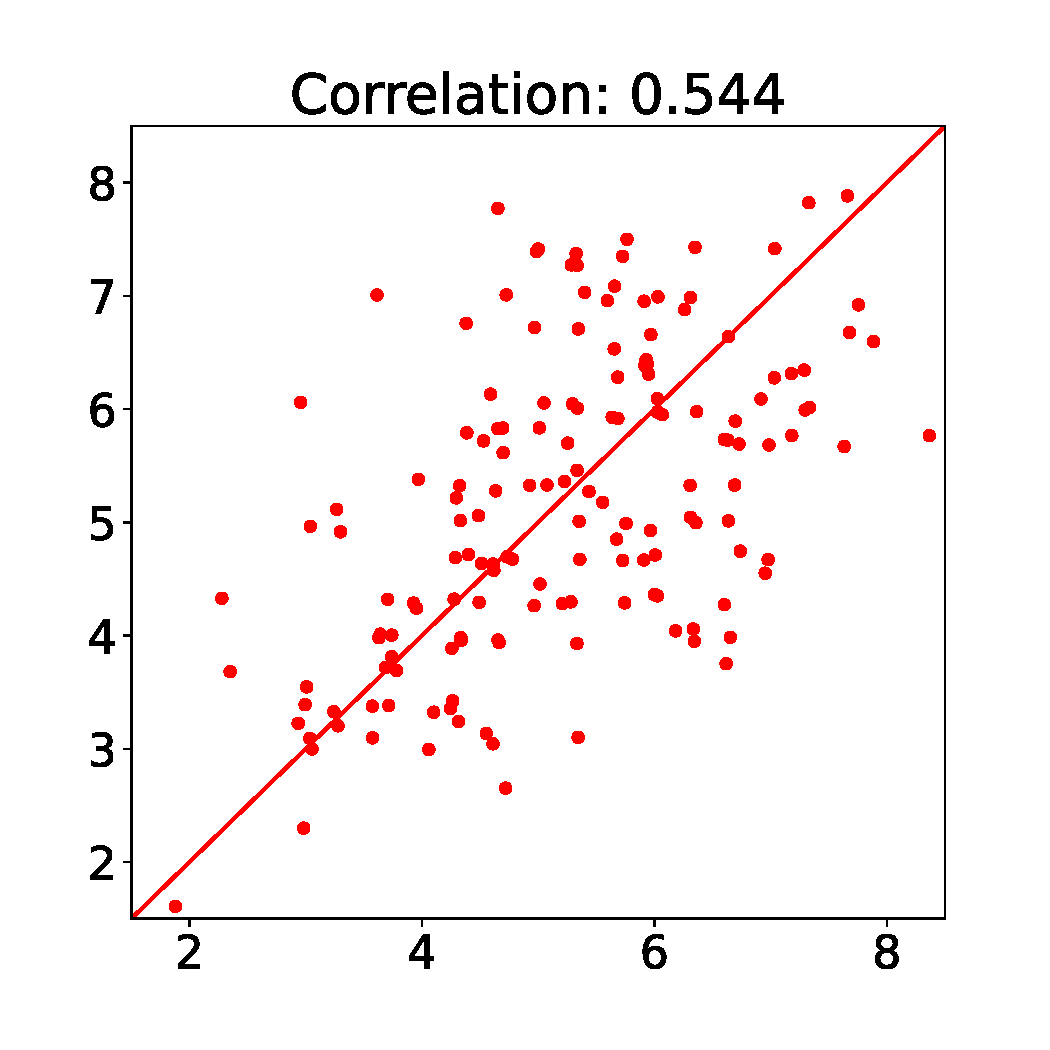
\includegraphics[width=0.60\textwidth]{diagrams/neurips/quality-correlation.pdf}


\caption{Correlation between reviewer scores across the duplicated committes (scores have jitter added to prevent too many points sitting on top of each other).}
\label{quality-correlation}
\end{figure}

Similarly for the calibrated quality of the papers.

\begin{figure}[htb]
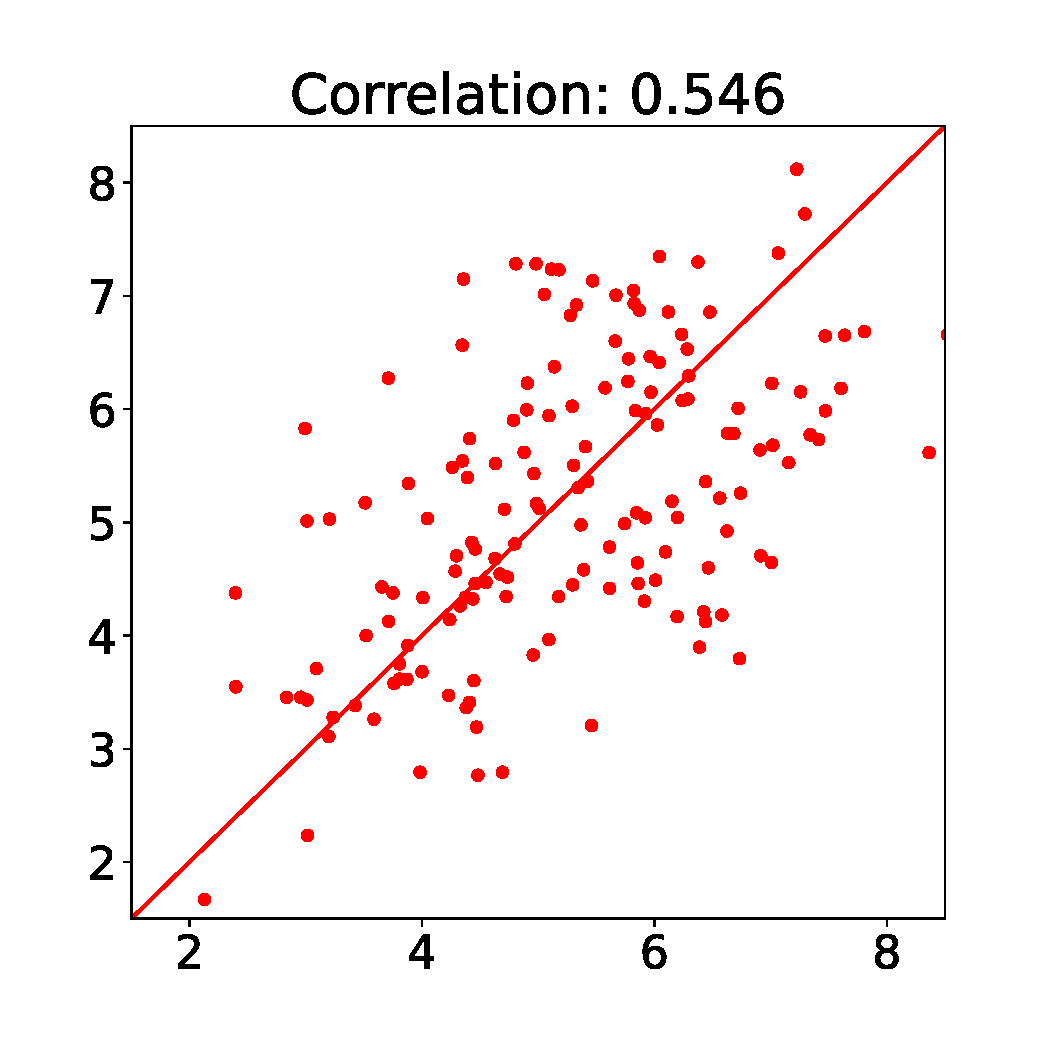
\includegraphics[width=0.60\textwidth]{diagrams/neurips/calibrated-quality-correlation.pdf}


\caption{Correlation between *calibrated* reviewer scores across the two independent committees.}
\label{calibrated-quality-correlation}
\end{figure}

\begin{Shaded}
\begin{Highlighting}[]
\CommentTok{\# Apply Laplace smoothing to accept probabilities before incorporating them.}
\NormalTok{revs }\OperatorTok{=}\NormalTok{ r.join((prob\_accept}\OperatorTok{+}\FloatTok{0.0002}\NormalTok{)}\OperatorTok{/}\FloatTok{1.001}\NormalTok{, on}\OperatorTok{=}\StringTok{\textquotesingle{}PaperID\textquotesingle{}}\NormalTok{).join(reviewer\_bias, on}\OperatorTok{=}\StringTok{\textquotesingle{}Email\textquotesingle{}}\NormalTok{).join(papers.papers[}\StringTok{\textquotesingle{}Number Of Discussions\textquotesingle{}}\NormalTok{], on}\OperatorTok{=}\StringTok{\textquotesingle{}PaperID\textquotesingle{}}\NormalTok{).join(reviewer\_bias\_std, on}\OperatorTok{=}\StringTok{\textquotesingle{}Email\textquotesingle{}}\NormalTok{).sort\_values(by}\OperatorTok{=}\NormalTok{[}\StringTok{\textquotesingle{}AcceptProbability\textquotesingle{}}\NormalTok{,}\StringTok{\textquotesingle{}PaperID\textquotesingle{}}\NormalTok{, }\StringTok{\textquotesingle{}CalibratedQuality\textquotesingle{}}\NormalTok{], ascending}\OperatorTok{=}\VariableTok{False}\NormalTok{)}
\NormalTok{revs.set\_index([}\StringTok{\textquotesingle{}PaperID\textquotesingle{}}\NormalTok{], inplace}\OperatorTok{=}\VariableTok{True}\NormalTok{)}
\KeywordTok{def}\NormalTok{ len\_comments(x):}
    \ControlFlowTok{return} \BuiltInTok{len}\NormalTok{(x.Comments)}
\NormalTok{revs[}\StringTok{\textquotesingle{}comment\_length\textquotesingle{}}\NormalTok{]}\OperatorTok{=}\NormalTok{revs.}\BuiltInTok{apply}\NormalTok{(len\_comments, axis}\OperatorTok{=}\DecValTok{1}\NormalTok{)}
\CommentTok{\# Save the computed information to disk}
\CommentTok{\#revs.to\_csv(os.path.join(cu.cmt\_data\_directory, date + \textquotesingle{}\_processed\_reviews.csv\textquotesingle{}), encoding=\textquotesingle{}utf{-}8\textquotesingle{})}
\end{Highlighting}
\end{Shaded}

\hypertarget{conference-simulation}{%
\subsection{Conference Simulation}\label{conference-simulation}}

\begin{flushright}
[\href{https://github.com/lawrennd/talks/edit/gh-pages/_neurips/includes/neurips-simulation.md}{edit}]
\end{flushright}

Given the realisation that roughly 50\% of the score seems to be
`subjective' and 50\% of the score seems to be `objective', then we can
simulate the conference and see what it does for the consistency of
accepts for different probability of accept.

\begin{Shaded}
\begin{Highlighting}[]
\ImportTok{import}\NormalTok{ numpy }\ImportTok{as}\NormalTok{ np}
\end{Highlighting}
\end{Shaded}

\begin{Shaded}
\begin{Highlighting}[]
\NormalTok{samples }\OperatorTok{=} \DecValTok{100000}
\NormalTok{subjectivity\_portion }\OperatorTok{=} \FloatTok{0.5}
\end{Highlighting}
\end{Shaded}

\begin{Shaded}
\begin{Highlighting}[]
\NormalTok{accept\_rates }\OperatorTok{=}\NormalTok{ [}\FloatTok{0.05}\NormalTok{, }\FloatTok{0.1}\NormalTok{, }\FloatTok{0.15}\NormalTok{, }\FloatTok{0.2}\NormalTok{, }\FloatTok{0.25}\NormalTok{, }\FloatTok{0.3}\NormalTok{, }\FloatTok{0.35}\NormalTok{, }\FloatTok{0.4}\NormalTok{, }\FloatTok{0.45}\NormalTok{, }\FloatTok{0.5}\NormalTok{, }\FloatTok{0.55}\NormalTok{, }\FloatTok{0.6}\NormalTok{, }\FloatTok{0.65}\NormalTok{, }\FloatTok{0.7}\NormalTok{, }\FloatTok{0.75}\NormalTok{, }\FloatTok{0.8}\NormalTok{, }\FloatTok{0.85}\NormalTok{, }\FloatTok{0.9}\NormalTok{, }\FloatTok{0.95}\NormalTok{, }\FloatTok{1.0}\NormalTok{]}
\NormalTok{consistent\_accepts }\OperatorTok{=}\NormalTok{ []}
\ControlFlowTok{for}\NormalTok{ accept\_rate }\KeywordTok{in}\NormalTok{ accept\_rates:}
\NormalTok{    score\_1 }\OperatorTok{=}\NormalTok{ []}
\NormalTok{    score\_2 }\OperatorTok{=}\NormalTok{ []}
    \ControlFlowTok{for}\NormalTok{ i }\KeywordTok{in} \BuiltInTok{range}\NormalTok{(samples):}
\NormalTok{        objective }\OperatorTok{=}\NormalTok{ (}\DecValTok{1}\OperatorTok{{-}}\NormalTok{subjectivity\_portion)}\OperatorTok{*}\NormalTok{np.random.randn()}
\NormalTok{        score\_1.append(objective }\OperatorTok{+}\NormalTok{ subjectivity\_portion}\OperatorTok{*}\NormalTok{np.random.randn())}
\NormalTok{        score\_2.append(objective }\OperatorTok{+}\NormalTok{ subjectivity\_portion}\OperatorTok{*}\NormalTok{np.random.randn())}

\NormalTok{    score\_1 }\OperatorTok{=}\NormalTok{ np.asarray(score\_1)}
\NormalTok{    score\_2 }\OperatorTok{=}\NormalTok{ np.asarray(score\_2)}

\NormalTok{    accept\_1 }\OperatorTok{=}\NormalTok{ score\_1.argsort()[:}\BuiltInTok{int}\NormalTok{(samples}\OperatorTok{*}\NormalTok{accept\_rate)]}
\NormalTok{    accept\_2 }\OperatorTok{=}\NormalTok{ score\_2.argsort()[:}\BuiltInTok{int}\NormalTok{(samples}\OperatorTok{*}\NormalTok{accept\_rate)]}

\NormalTok{    consistent\_accept }\OperatorTok{=} \BuiltInTok{len}\NormalTok{(}\BuiltInTok{set}\NormalTok{(accept\_1).intersection(}\BuiltInTok{set}\NormalTok{(accept\_2)))}
\NormalTok{    consistent\_accepts.append(consistent\_accept}\OperatorTok{/}\NormalTok{(samples}\OperatorTok{*}\NormalTok{accept\_rate))}
    \BuiltInTok{print}\NormalTok{(}\StringTok{\textquotesingle{}Percentage consistently accepted: }\SpecialCharTok{\{prop\}}\StringTok{\textquotesingle{}}\NormalTok{.}\BuiltInTok{format}\NormalTok{(prop}\OperatorTok{=}\NormalTok{consistent\_accept}\OperatorTok{/}\NormalTok{(samples}\OperatorTok{*}\NormalTok{accept\_rate)))}

\NormalTok{consistent\_accepts }\OperatorTok{=}\NormalTok{ np.array(consistent\_accepts)}
\NormalTok{accept\_rate }\OperatorTok{=}\NormalTok{ np.array(accept\_rate)}
\end{Highlighting}
\end{Shaded}

\textbackslash begin\{figure\}{[}htb{]}
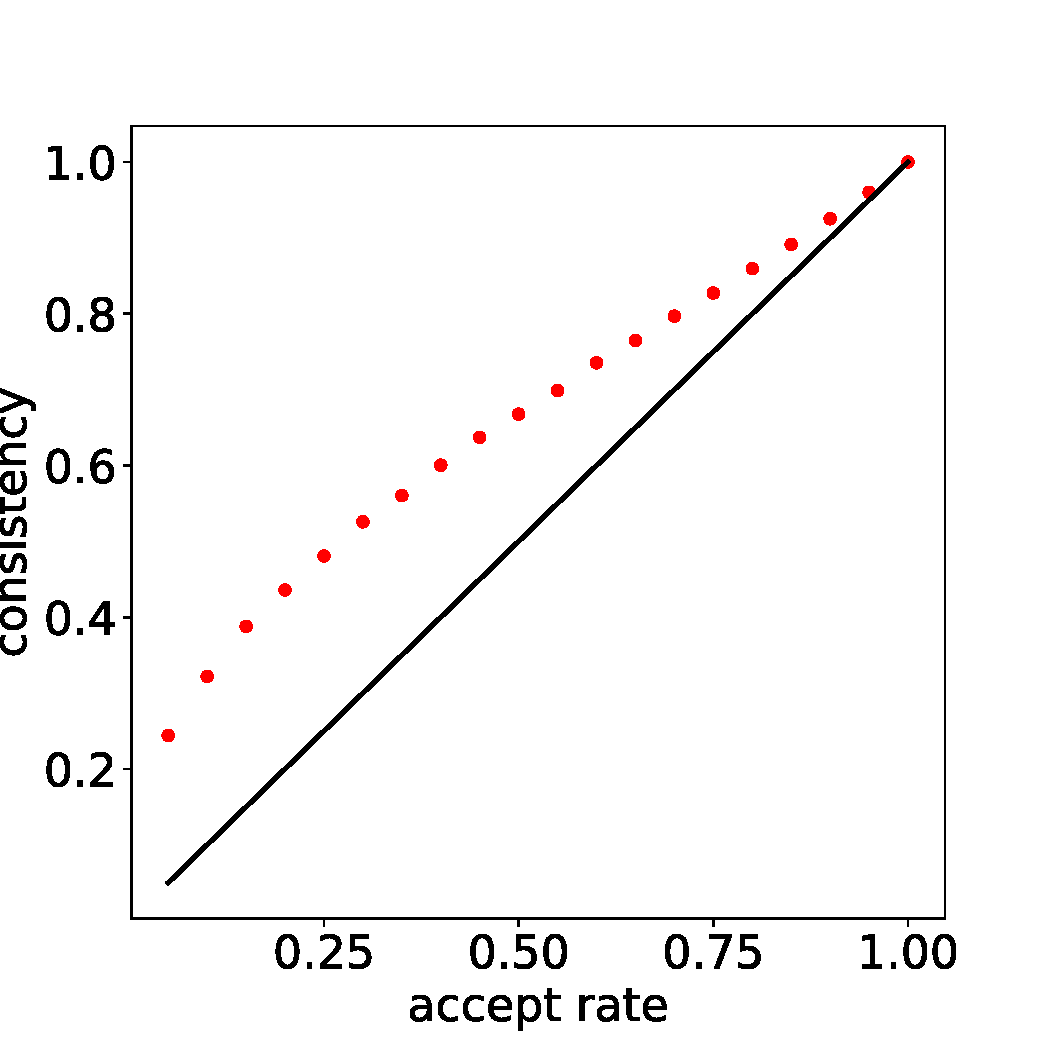
\includegraphics[width=0.50\textwidth]{diagrams/neurips/consistency-vs-accept-rate.pdf}

\textbackslash caption\{Plot of the accept rate vs the consistency of
the conference for 50\% subjectivity.\}
\label{consistency-vs-accept-rate} \textbackslash end\{figure\}

\textbackslash begin\{figure\}{[}htb{]}
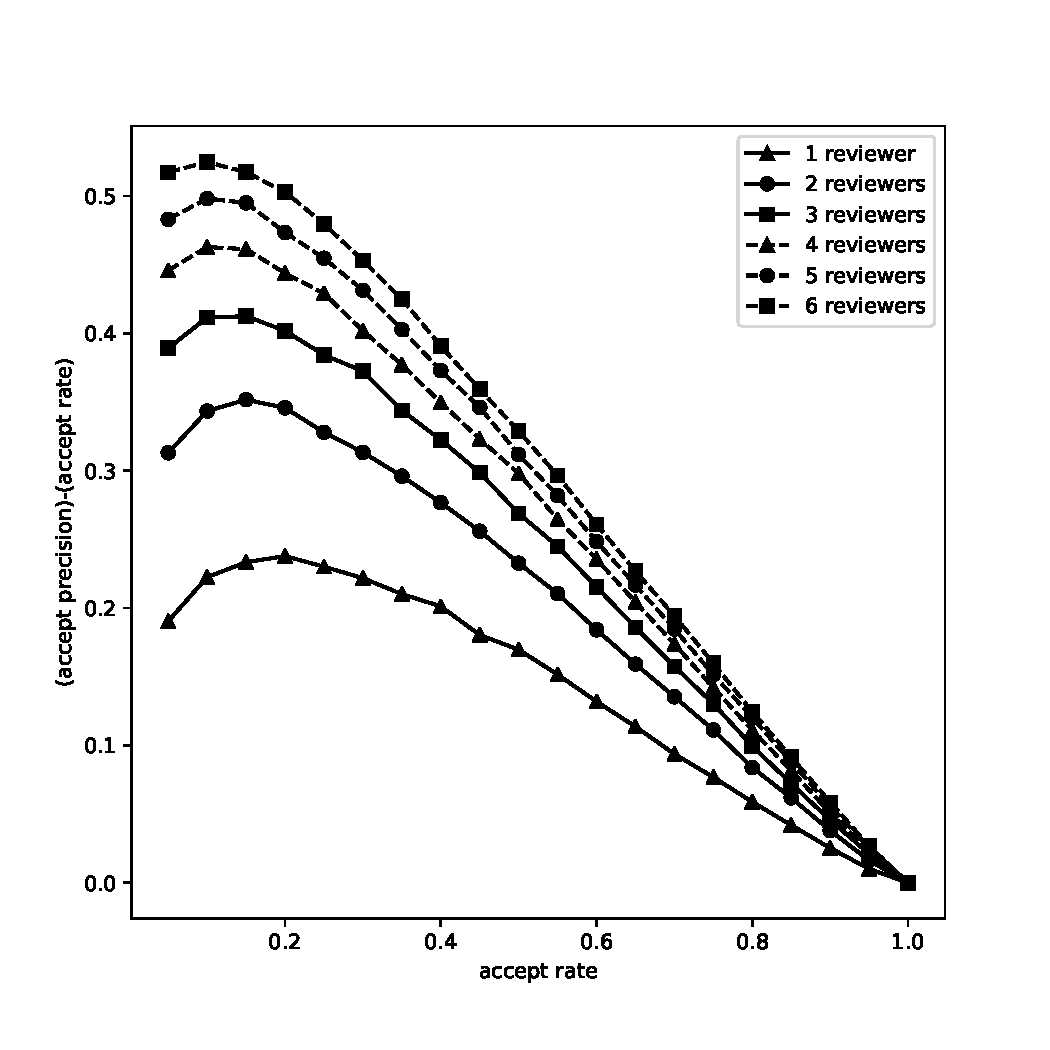
\includegraphics[width=0.50\textwidth]{diagrams/neurips/gain-in-consistency.pdf}

\textbackslash caption\{Plot of the accept rate vs gain in consistency
over a random conference for 50\% subjectivity.\}
\label{gain-in-consistency} \textbackslash end\{figure\}

\hypertarget{where-do-rejected-papers-go}{%
\subsection{Where do Rejected Papers
Go?}\label{where-do-rejected-papers-go}}

\begin{flushright}
[\href{https://github.com/lawrennd/talks/edit/gh-pages/_neurips/includes/where-do-the-rejected-papers-go.md}{edit}]
\end{flushright}

\begin{Shaded}
\begin{Highlighting}[]
\ImportTok{import}\NormalTok{ os}
\ImportTok{import}\NormalTok{ yaml}
\end{Highlighting}
\end{Shaded}

\begin{Shaded}
\begin{Highlighting}[]
\ControlFlowTok{with} \BuiltInTok{open}\NormalTok{(os.path.join(nipsy.review\_store, nipsy.outlet\_name\_mapping), }\StringTok{\textquotesingle{}r\textquotesingle{}}\NormalTok{) }\ImportTok{as}\NormalTok{ f:}
\NormalTok{    mapping }\OperatorTok{=}\NormalTok{ yaml.load(f, Loader}\OperatorTok{=}\NormalTok{yaml.FullLoader)}


\NormalTok{date }\OperatorTok{=} \StringTok{"2021{-}06{-}11"}

\NormalTok{citations }\OperatorTok{=}\NormalTok{ nipsy.load\_citation\_counts(date}\OperatorTok{=}\NormalTok{date)}
\NormalTok{decisions }\OperatorTok{=}\NormalTok{ nipsy.load\_decisions()}
\NormalTok{nipsy.augment\_decisions(decisions)}
\NormalTok{joindf }\OperatorTok{=}\NormalTok{ nipsy.join\_decisions\_citations(decisions, citations)}

\NormalTok{joindf[}\StringTok{\textquotesingle{}short\_venue\textquotesingle{}}\NormalTok{] }\OperatorTok{=}\NormalTok{ joindf.venue.replace(mapping)}
\end{Highlighting}
\end{Shaded}

\begin{figure}[htb]
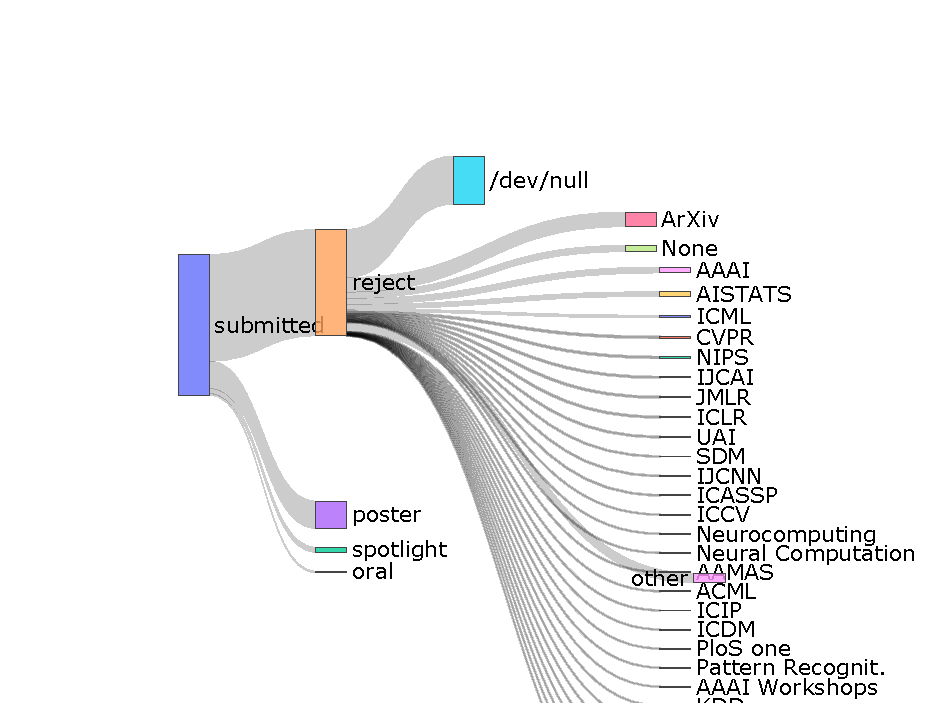
\includegraphics[width=0.80\textwidth]{diagrams/neurips/where-do-neurips-papers-go.pdf}


\caption{Sankey diagram showing the flow of NeurIPS papers through the system from submission to eventual publication.}
\label{where-do-neurips-papers-go}
\end{figure}

\}

\hypertarget{effect-of-late-reviews}{%
\subsection{Effect of Late Reviews}\label{effect-of-late-reviews}}

\begin{flushright}
[\href{https://github.com/lawrennd/talks/edit/gh-pages/_neurips/includes/effect-of-late-reviewers.md}{edit}]
\end{flushright}

This notebook analyzes the reduction in reviewer confidence between
reviewers that submit their reviews early and those that arrive late.
The reviews are first loaded in from files Corinna and Neil saved and
stored in a pickle. The function for doing that is
\texttt{nips.load\_review\_history}.

\begin{Shaded}
\begin{Highlighting}[]
\ImportTok{import}\NormalTok{ cmtutils }\ImportTok{as}\NormalTok{ cu}
\ImportTok{import}\NormalTok{ cmtutils.nipsy }\ImportTok{as}\NormalTok{ nipsy }
\ImportTok{import}\NormalTok{ cmtutils.plot }\ImportTok{as}\NormalTok{ plot}

\ImportTok{import}\NormalTok{ os}
\ImportTok{import}\NormalTok{ pandas }\ImportTok{as}\NormalTok{ pd}
\ImportTok{import}\NormalTok{ numpy }\ImportTok{as}\NormalTok{ np}
\end{Highlighting}
\end{Shaded}

\begin{Shaded}
\begin{Highlighting}[]
\NormalTok{reviews }\OperatorTok{=}\NormalTok{ nipsy.load\_review\_history()}
\end{Highlighting}
\end{Shaded}

\hypertarget{review-submission-times}{%
\subsection{Review Submission Times}\label{review-submission-times}}

All reviews are now in pandas data frame called reviews, they are ready
for processing. First of all, let's take a look at when the reviews were
submitted. The function \texttt{nipsy.reviews\_before} gives a snapshot
of the reviews as they stood at a particular date. So we simply create a
data series across the data range of reviews
(\texttt{nipsy.review\_data\_range}) that shows the counts.

\begin{Shaded}
\begin{Highlighting}[]
\NormalTok{review\_count }\OperatorTok{=}\NormalTok{ pd.Series(index}\OperatorTok{=}\NormalTok{nipsy.review\_date\_range)}
\ControlFlowTok{for}\NormalTok{ date }\KeywordTok{in}\NormalTok{ nipsy.review\_date\_range:}
\NormalTok{    review\_count.loc[date] }\OperatorTok{=}\NormalTok{ nipsy.reviews\_before(reviews, date).Quality.shape[}\DecValTok{0}\NormalTok{]}
\end{Highlighting}
\end{Shaded}

\begin{figure}[htb]
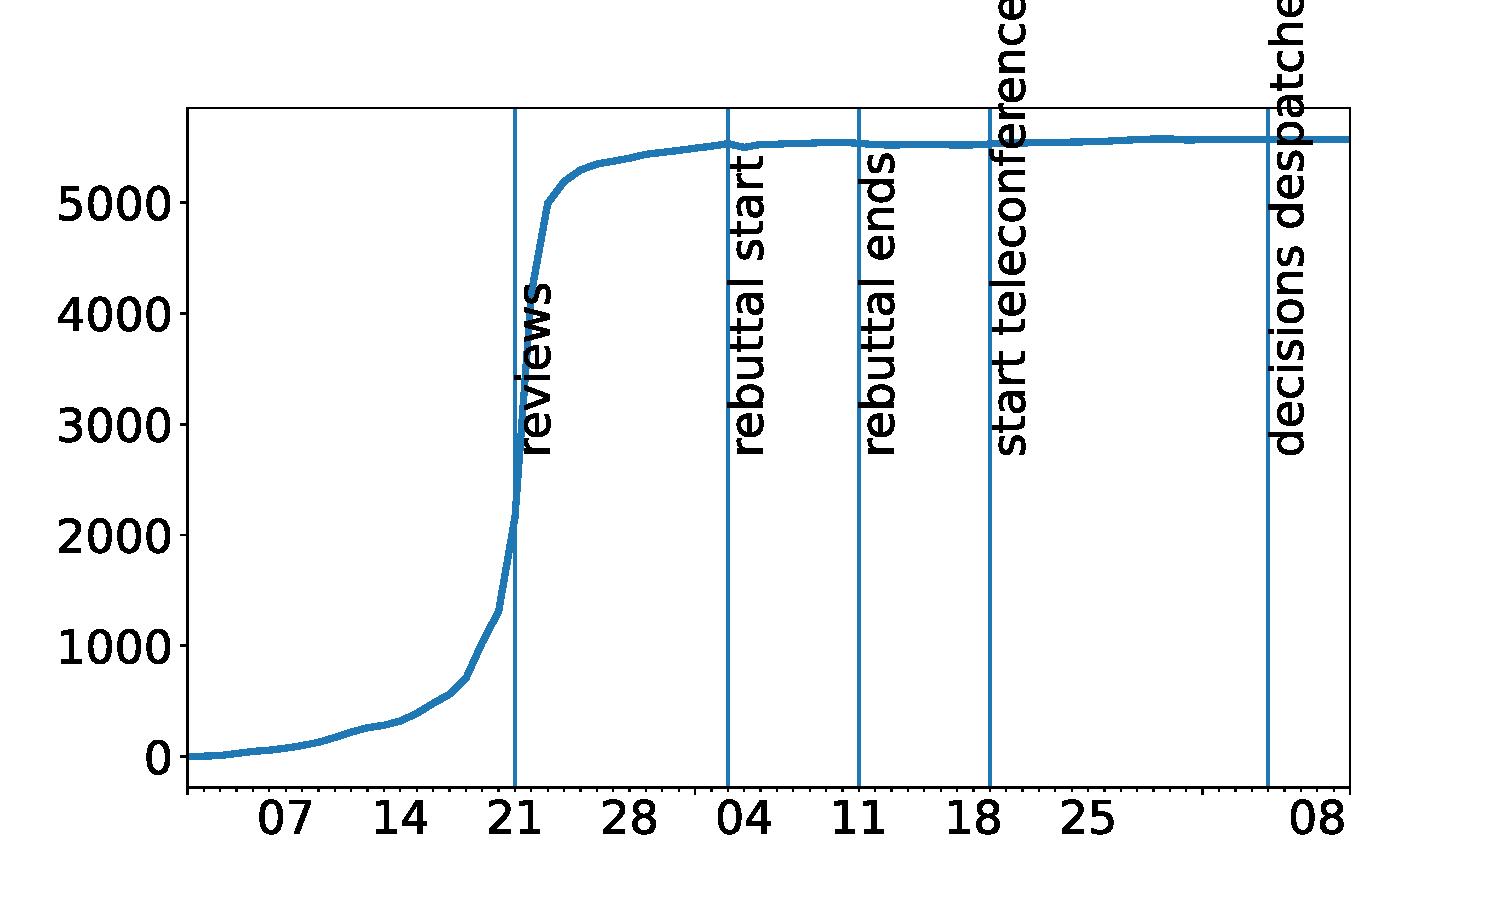
\includegraphics[width=0.70\textwidth]{diagrams/neurips/review-count.pdf}


\caption{Cumulative count of number of received reviews over time.}
\label{review-count}
\end{figure}

We worked hard to try and ensure that all papers had three reviews
before the start of the rebuttal. This next plot shows the numbers of
papers that had less than three reviews across the review period. First
let's look at the overall statistics of what the count of reviewers per
paper were. Below we plot mean, maximum, median and minimum over time.

\begin{Shaded}
\begin{Highlighting}[]
\NormalTok{lastseen }\OperatorTok{=}\NormalTok{ reviews.drop\_duplicates(subset}\OperatorTok{=}\StringTok{\textquotesingle{}ID\textquotesingle{}}\NormalTok{).set\_index(}\StringTok{\textquotesingle{}ID\textquotesingle{}}\NormalTok{)}
\NormalTok{lastseen }\OperatorTok{=}\NormalTok{ lastseen[}\StringTok{\textquotesingle{}LastSeen\textquotesingle{}}\NormalTok{]}

\NormalTok{review\_count }\OperatorTok{=}\NormalTok{ pd.DataFrame(index}\OperatorTok{=}\NormalTok{reviews.ID.unique(), columns}\OperatorTok{=}\NormalTok{nipsy.review\_date\_range)}
\ControlFlowTok{for}\NormalTok{ date }\KeywordTok{in}\NormalTok{ nipsy.review\_date\_range:}
\NormalTok{    counts }\OperatorTok{=}\NormalTok{ nipsy.reviews\_status(reviews, date, column}\OperatorTok{=}\StringTok{\textquotesingle{}Quality\textquotesingle{}}\NormalTok{).count(level}\OperatorTok{=}\StringTok{\textquotesingle{}ID\textquotesingle{}}\NormalTok{)}
\NormalTok{    review\_count[date] }\OperatorTok{=}\NormalTok{ counts.fillna(}\DecValTok{0}\NormalTok{)}
\NormalTok{review\_count.fillna(}\DecValTok{0}\NormalTok{, inplace}\OperatorTok{=}\VariableTok{True}\NormalTok{)    }
\NormalTok{review\_count }\OperatorTok{=}\NormalTok{ review\_count.T}
\ControlFlowTok{for}\NormalTok{ col }\KeywordTok{in}\NormalTok{ review\_count.columns:}
    \ControlFlowTok{if}\NormalTok{ pd.notnull(lastseen[col]):}
\NormalTok{        review\_count[col][review\_count.index}\OperatorTok{\textgreater{}}\NormalTok{lastseen[col]] }\OperatorTok{=}\NormalTok{ np.NaN}
        
\NormalTok{review\_count }\OperatorTok{=}\NormalTok{ review\_count.T}
\end{Highlighting}
\end{Shaded}

\begin{figure}[htb]
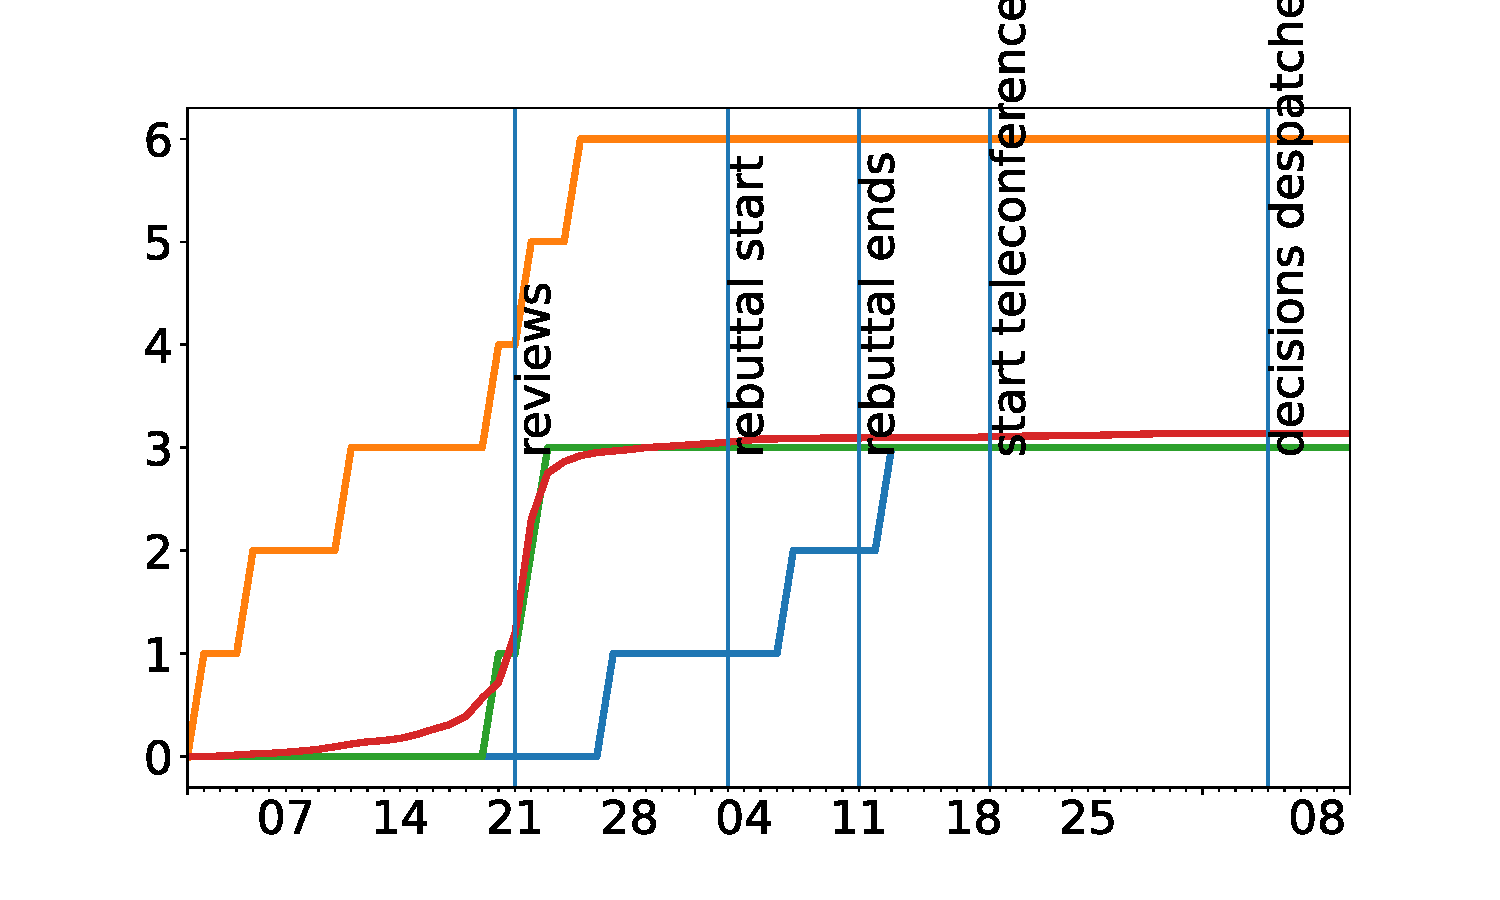
\includegraphics[width=0.70\textwidth]{diagrams/neurips/number-of-reviews-over-time.pdf}


\caption{Plot representing number of reviewers per paper over time showing maximum number of reviewers per paper, minimum, median and mean. }
\label{number-of-reviews-over-time}
\end{figure}

But perhaps the more important measure is how many papers had less than
3 reviewers over time. In this plot you can see that by the time
rebuttal starts almost all papers have three reviewers.

\begin{Shaded}
\begin{Highlighting}[]
\NormalTok{count }\OperatorTok{=}\NormalTok{ pd.Series(index}\OperatorTok{=}\NormalTok{nipsy.review\_date\_range)}
\ControlFlowTok{for}\NormalTok{ date }\KeywordTok{in}\NormalTok{ nipsy.review\_date\_range:}
\NormalTok{    count[date] }\OperatorTok{=}\NormalTok{ (review\_count[date]}\OperatorTok{\textless{}}\DecValTok{3}\NormalTok{).}\BuiltInTok{sum}\NormalTok{()}
\end{Highlighting}
\end{Shaded}

\begin{figure}[htb]
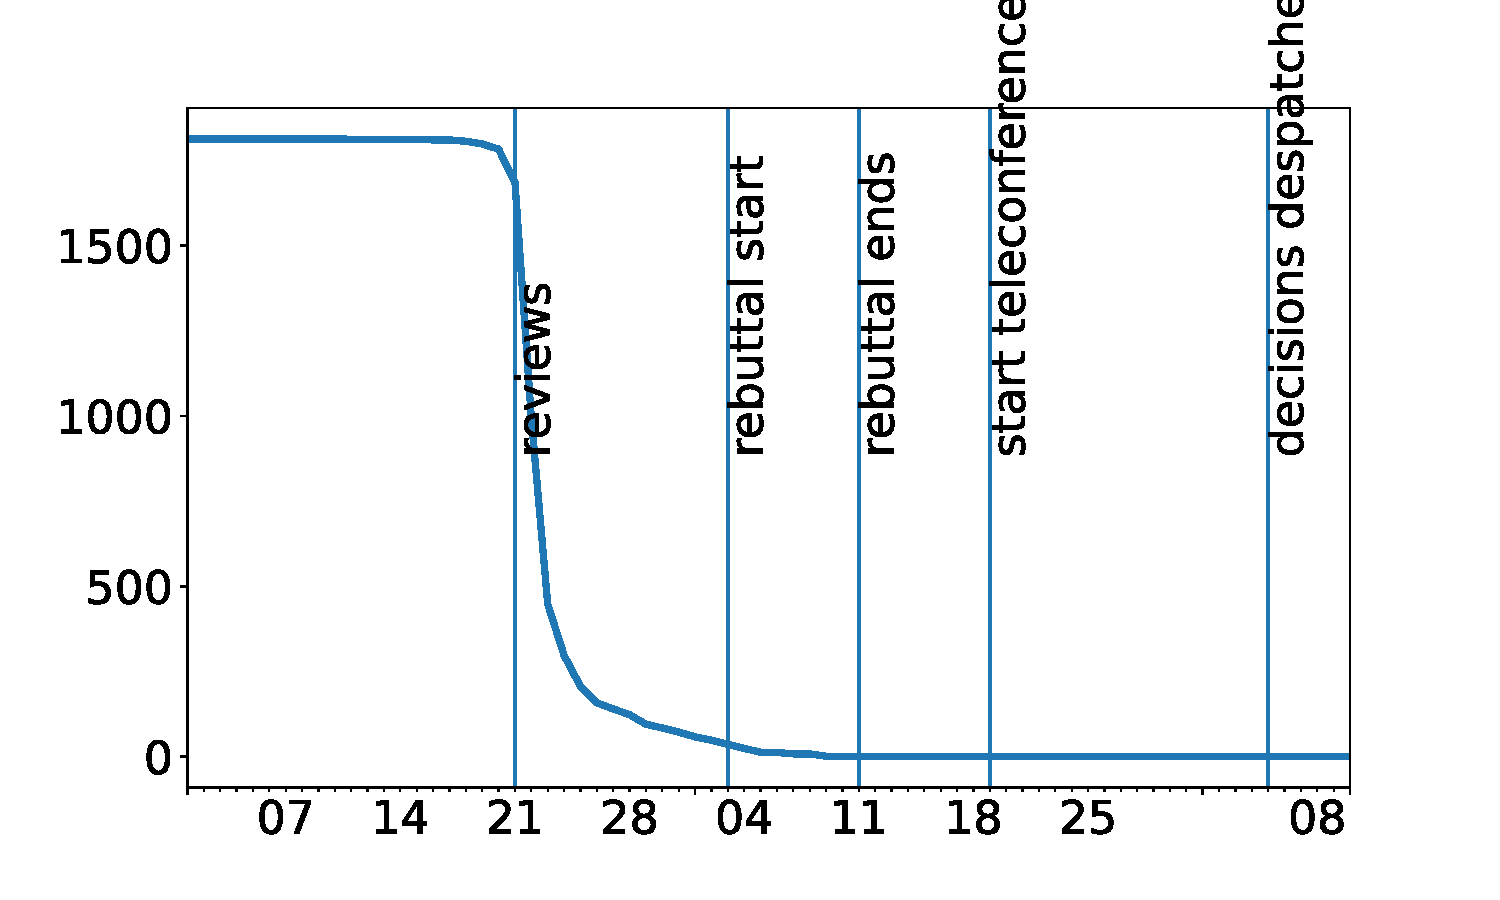
\includegraphics[width=0.70\textwidth]{diagrams/neurips/paper-short-reviews.pdf}


\caption{}
\label{paper-short-reviews}
\end{figure}

\hypertarget{review-confidence}{%
\subsection{Review Confidence}\label{review-confidence}}

Now we will check the confidence of reviews as the come in over time.
We've written a small helper function that looks in a four day window
around each time point and summarises the associated score (in the first
case, confidence, \texttt{Conf}) with its across the four day window and
95\% confidence intervals computed from the standard error of the mean
estimate.

\begin{figure}[htb]
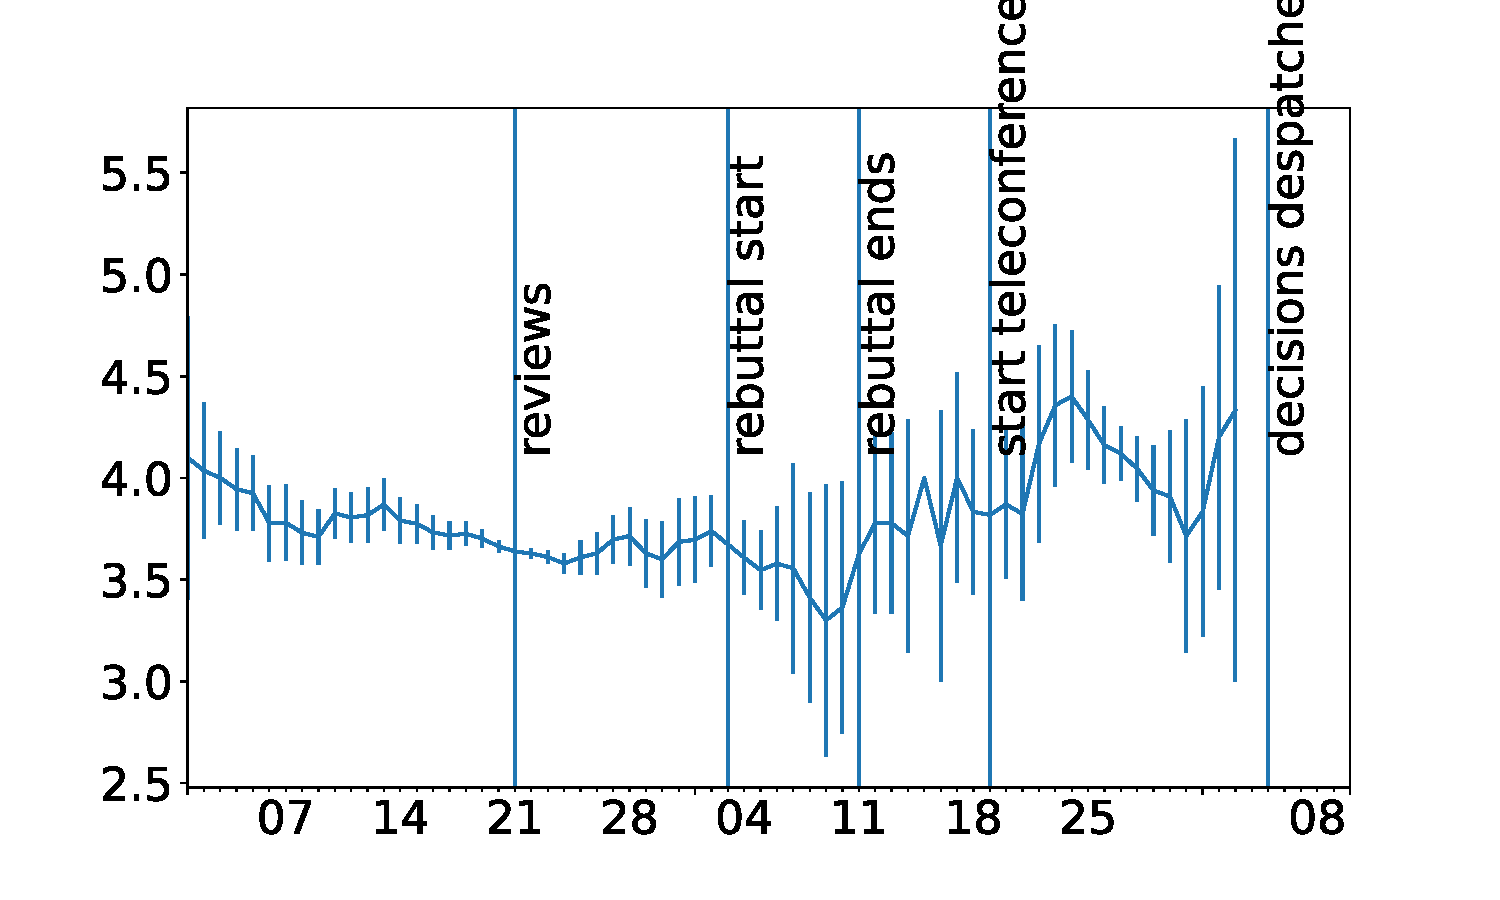
\includegraphics[width=0.70\textwidth]{diagrams/neurips/review-confidence-time.pdf}


\caption{}
\label{review-confidence-time}
\end{figure}

It looks like there might be a reduction in confidence as we pass the
review deadline on 21st July, but is the difference in confidence for
the reviews that came in later really significant?

We now simplify the question by looking at the average confidence for
reviews that arrived before 21st July (the reviewing deadline) and
reviews that arrived after the 21st July (i.e.~those that were chased or
were allocated late) but before the rebuttal period started (4th
August). Below we select these two groups and estimate the estimate of
the mean confidence with (again with error bars).

\begin{figure}[htb]
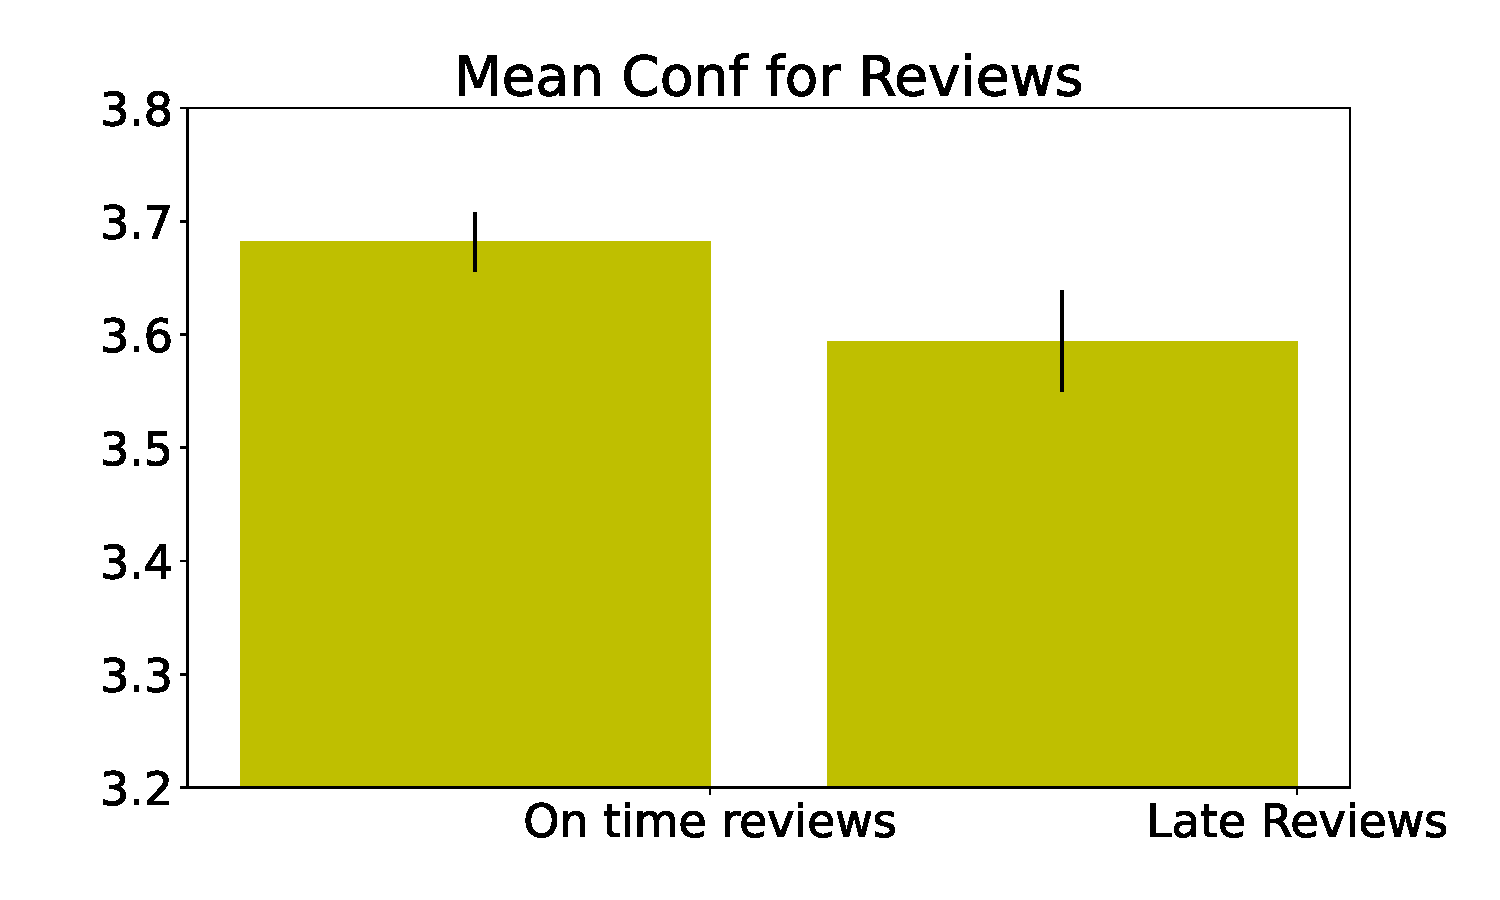
\includegraphics[width=0.50\textwidth]{diagrams/neurips/review-confidence-early-late.pdf}


\caption{}
\label{review-confidence-early-late}
\end{figure}

So it looks like there is a small but significant difference between the
average confidence of the submitted reviews before and after the
deadline, the statistical significance is confirmed with a \(t\)-test
with a \(p\)-value at 0.048\%. The magnitude of the difference is small
(about 0.1) but may indicate a tendency for later reviewers to be a
little more rushed.

\hypertarget{quality-score}{%
\subsubsection{Quality Score}\label{quality-score}}

This begs the question, is there an effect on the other scores of their
reviews which cover 'quality' and 'impact'. Quality of papers is scored
on a 10 point scale with a recommendation of 6 being accept and We can
form a similar plot for quality as follows.

\begin{figure}[htb]
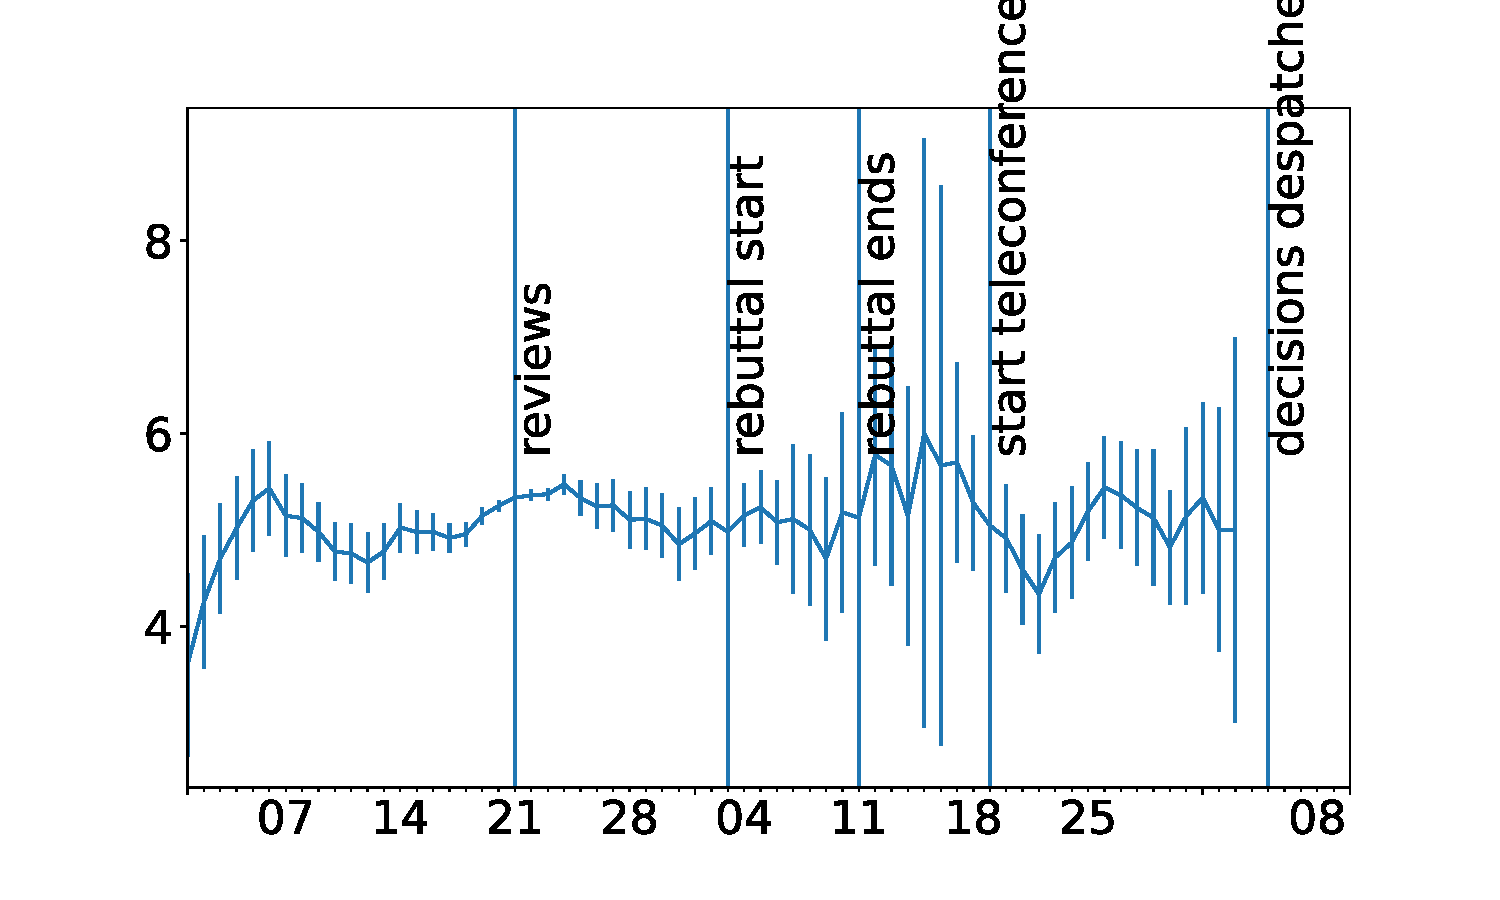
\includegraphics[width=0.70\textwidth]{diagrams/neurips/review-quality-time.pdf}


\caption{}
\label{review-quality-time}
\end{figure}

\begin{figure}[htb]
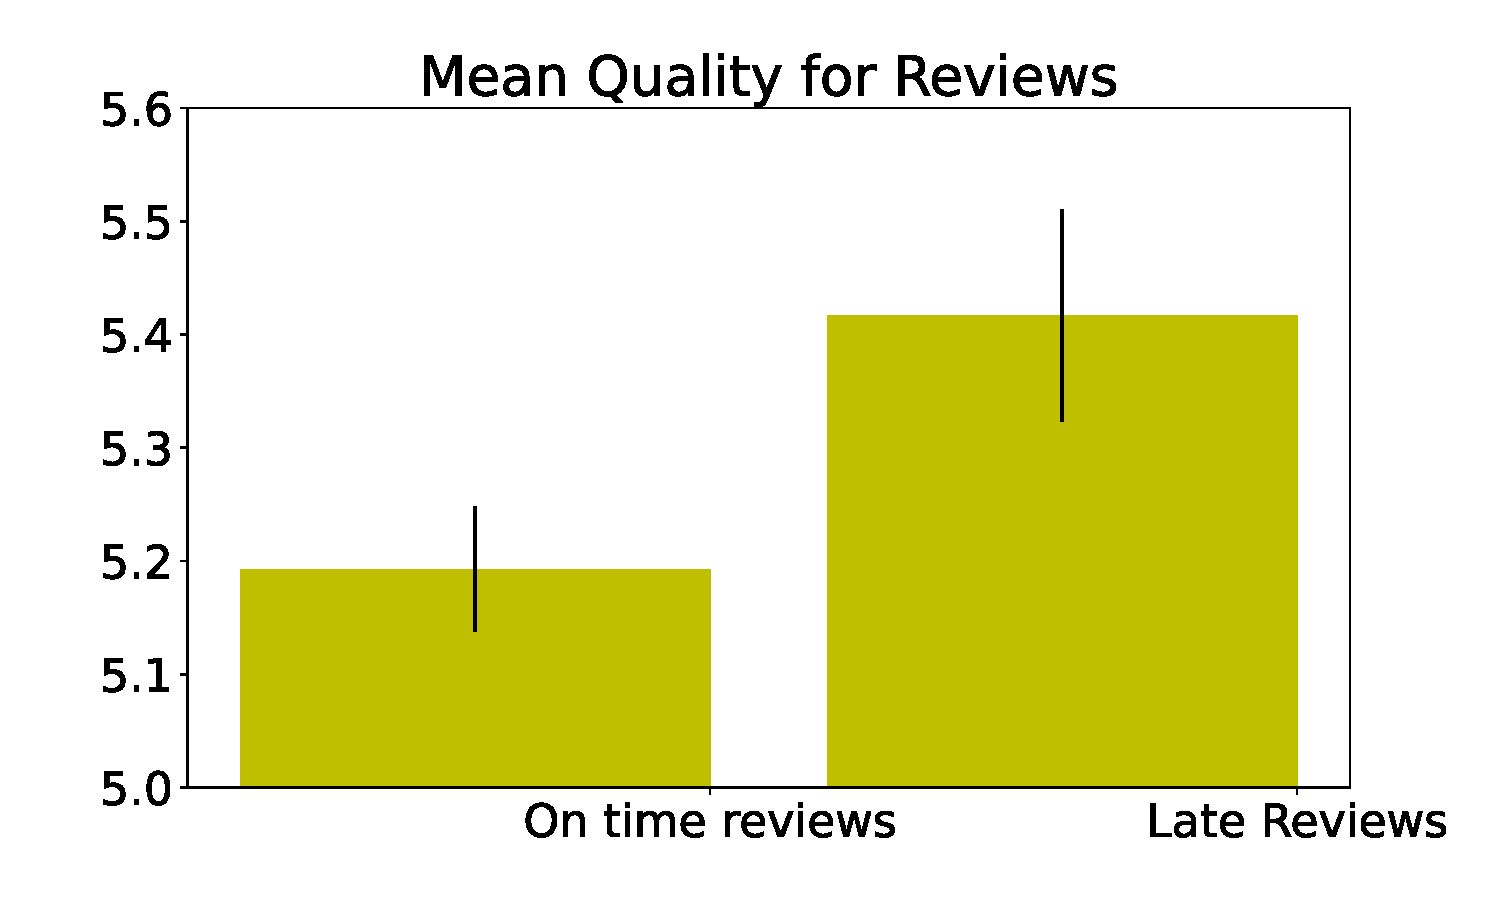
\includegraphics[width=0.50\textwidth]{diagrams/neurips/review-quality-early-late.pdf}


\caption{}
\label{review-quality-early-late}
\end{figure}

There is another statistically significant difference between perceived
quality scores after the reviewing deadline than before. On average
reviewers tend to be more generous in their quality perceptions when the
review is late. The \(p\)-value is computed as 0.007\%. We can also
check if there is a similar on the impact score. The impact score was
introduced by Ghahramani and Welling in an effort to get reviewers not
just to think about the technical side of the paper, but whether it is
driving the field forward. The score is binary, with 1 being for a paper
that is unlikey to have high impact and 2 being for a paper that is
likely to have a high impact.

\begin{figure}[htb]
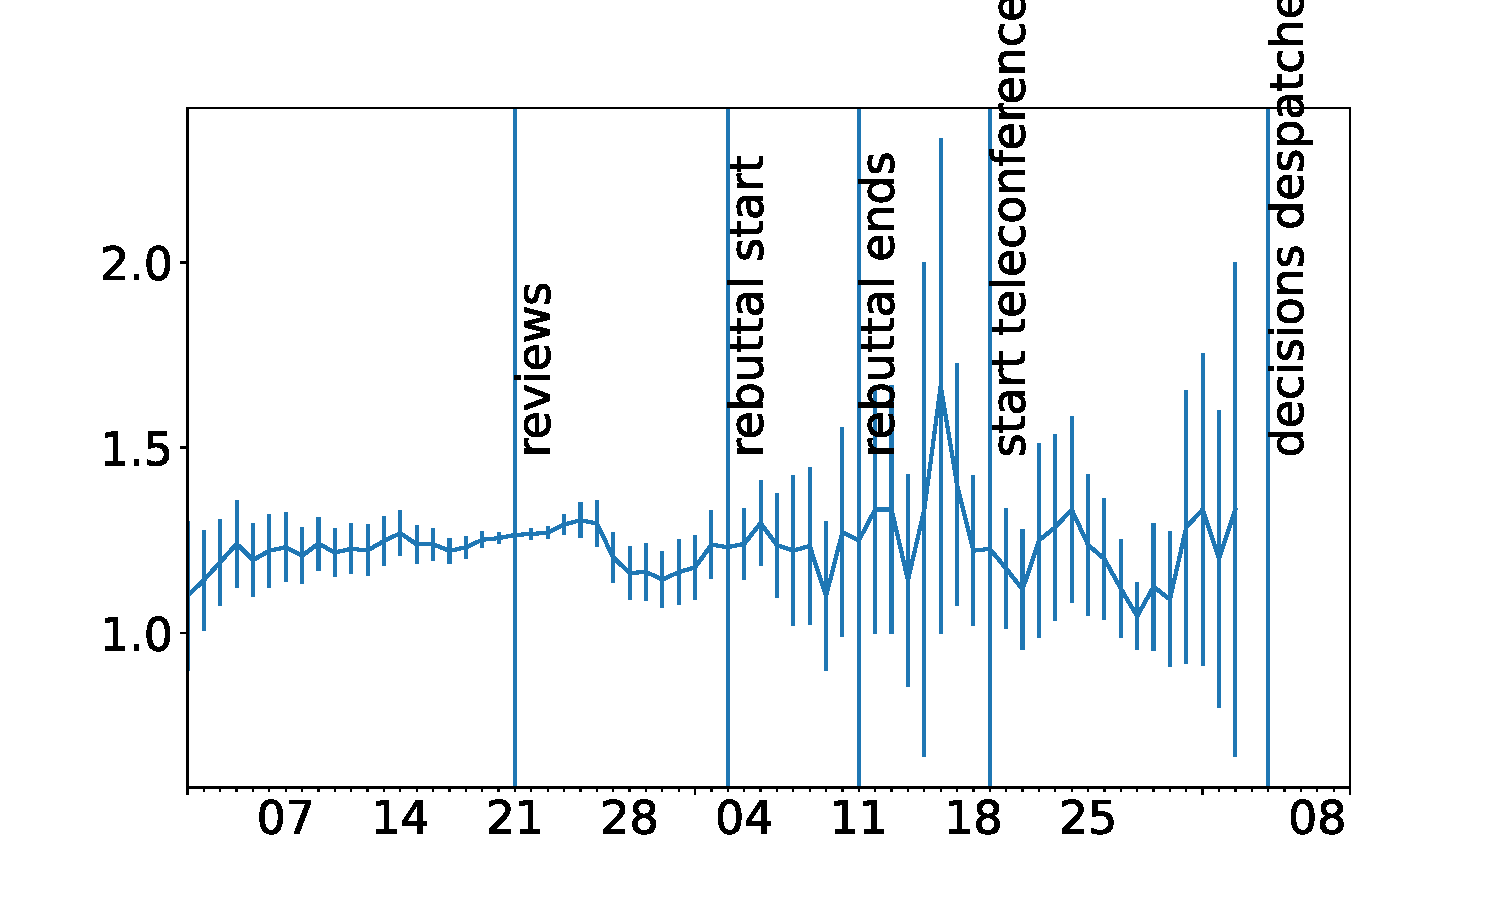
\includegraphics[width=0.70\textwidth]{diagrams/neurips/review-impact-time.pdf}


\caption{}
\label{review-impact-time}
\end{figure}

\begin{figure}[htb]
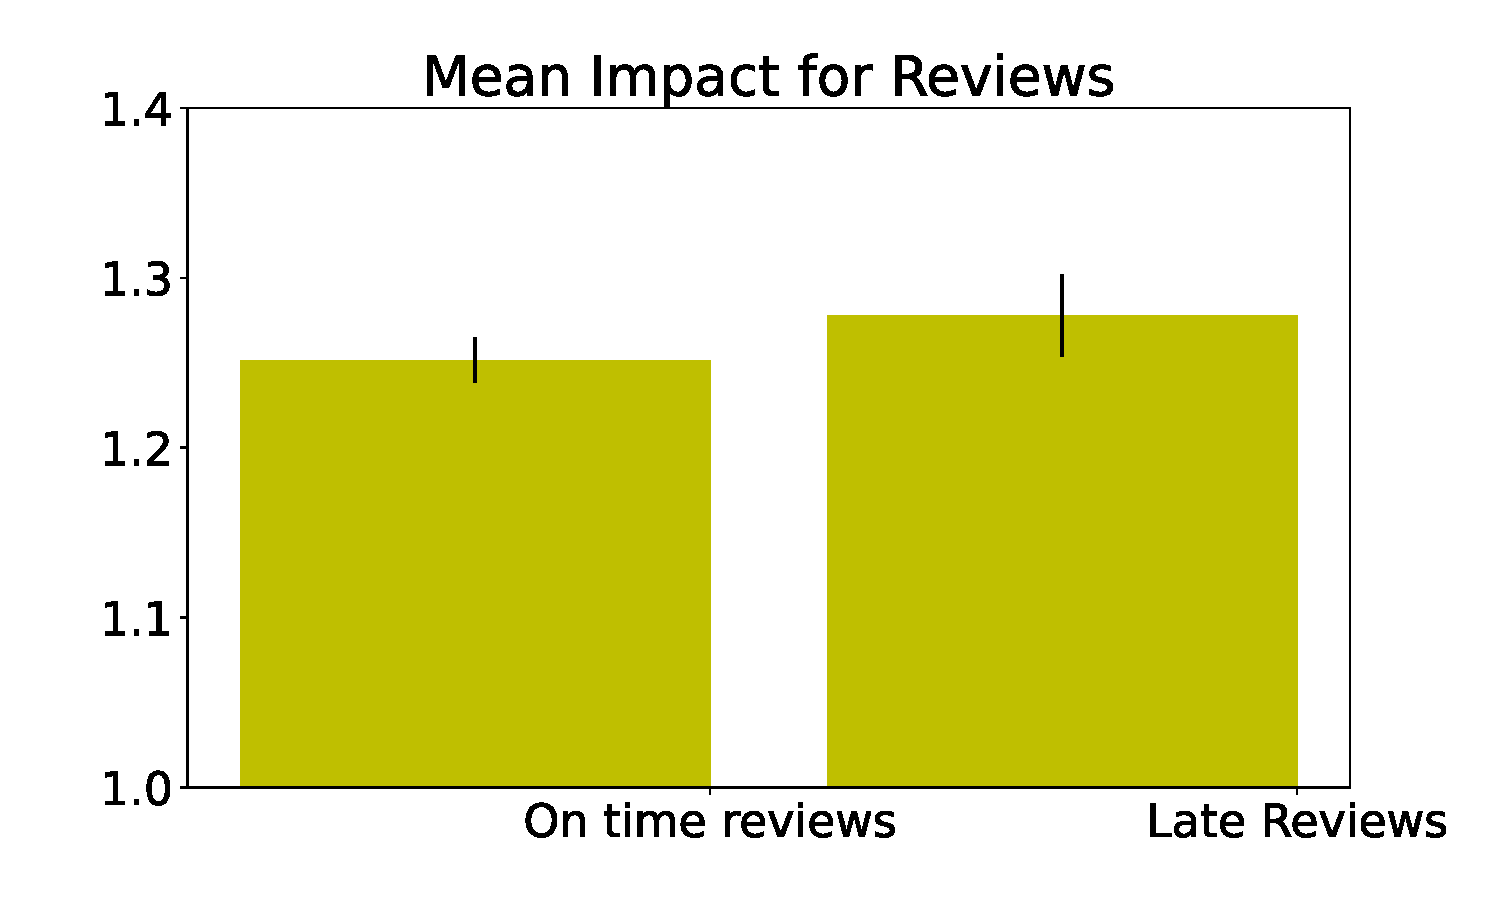
\includegraphics[width=0.50\textwidth]{diagrams/neurips/review-impact-early-late.pdf}


\caption{}
\label{review-impact-early-late}
\end{figure}

We find the difference is not quite statistically significant for the
impact score (\(p\)-value of 5.9\%), but if anything there is a trend to
have slightly higher impacts for later reviews.

\hypertarget{review-length}{%
\subsubsection{Review Length}\label{review-length}}

A final potential indicator of review quality is the length of the
reviews, we can check if there is a difference between the combined
length of the review summary and the main body comments for late and
early reviews.

\begin{figure}[htb]
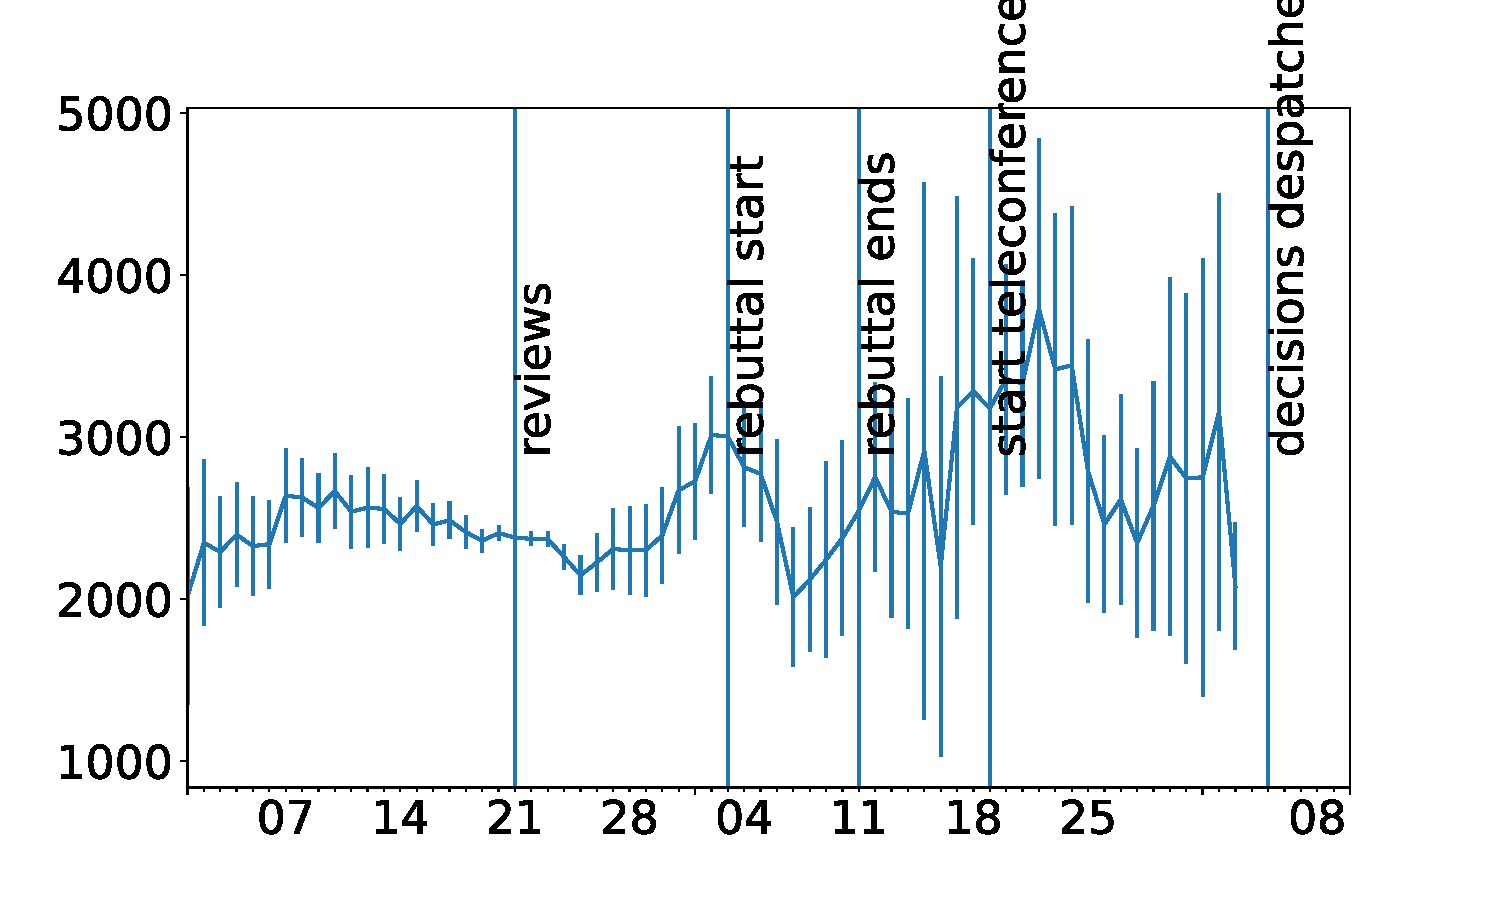
\includegraphics[width=0.70\textwidth]{diagrams/neurips/review-length-time.pdf}


\caption{}
\label{review-length-time}
\end{figure}

\begin{figure}[htb]
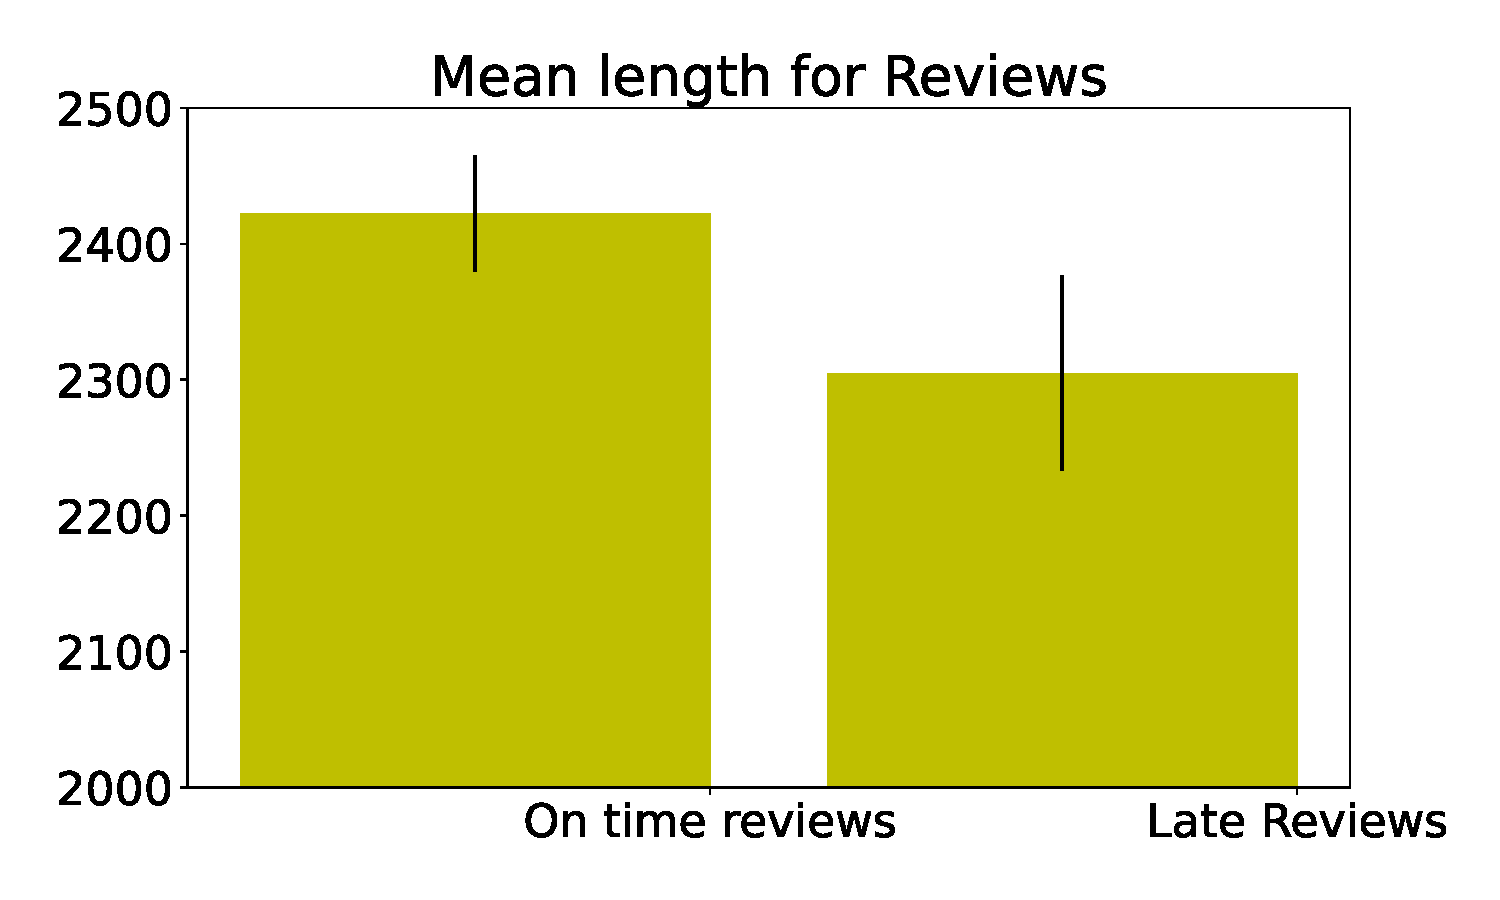
\includegraphics[width=0.50\textwidth]{diagrams/neurips/review-length-early-late.pdf}


\caption{}
\label{review-length-early-late}
\end{figure}

Once again we find a small but statitically significant difference,
here, as we might expect late reviews are shorter than those submitted
on time, by about 100 words in a 2,400 word review.

\begin{Shaded}
\begin{Highlighting}[]
\NormalTok{review\_quality }\OperatorTok{=}\NormalTok{ pd.DataFrame(index}\OperatorTok{=}\NormalTok{reviews.ID.unique(), columns}\OperatorTok{=}\NormalTok{nipsy.review\_date\_range)}
\ControlFlowTok{for}\NormalTok{ date }\KeywordTok{in}\NormalTok{ nipsy.review\_date\_range:}
\NormalTok{    qual }\OperatorTok{=}\NormalTok{ nipsy.reviews\_status(reviews, date, column}\OperatorTok{=}\StringTok{\textquotesingle{}Quality\textquotesingle{}}\NormalTok{)}
\NormalTok{    review\_quality[date] }\OperatorTok{=}\NormalTok{ qual.}\BuiltInTok{sum}\NormalTok{(level}\OperatorTok{=}\StringTok{\textquotesingle{}ID\textquotesingle{}}\NormalTok{)}\OperatorTok{/}\NormalTok{qual.count(level}\OperatorTok{=}\StringTok{\textquotesingle{}ID\textquotesingle{}}\NormalTok{) }\CommentTok{\# There\textquotesingle{}s a bug where mean doesn\textquotesingle{}t work in Pandas 1.2.4??}
\end{Highlighting}
\end{Shaded}

\begin{Shaded}
\begin{Highlighting}[]
\NormalTok{original\_pairs }\OperatorTok{=}\NormalTok{ pd.read\_csv(os.path.join(nipsy.review\_store, }\StringTok{\textquotesingle{}Duplicate\_PaperID\_Pairs.csv\textquotesingle{}}\NormalTok{), index\_col}\OperatorTok{=}\StringTok{\textquotesingle{}original\textquotesingle{}}\NormalTok{)}
\NormalTok{duplicate\_pairs }\OperatorTok{=}\NormalTok{ pd.read\_csv(os.path.join(nipsy.review\_store, }\StringTok{\textquotesingle{}Duplicate\_PaperID\_Pairs.csv\textquotesingle{}}\NormalTok{), index\_col}\OperatorTok{=}\StringTok{\textquotesingle{}duplicate\textquotesingle{}}\NormalTok{)}
\end{Highlighting}
\end{Shaded}

Perform an 'inner join' on duplicate papers and their originals with
their reviews, and set the index of the duplicated papers to match the
original. This gives us data frames with matching indices containing
scores over time of the duplicate and original papers.

\begin{Shaded}
\begin{Highlighting}[]
\NormalTok{duplicate\_reviews }\OperatorTok{=}\NormalTok{ duplicate\_pairs.join(review\_quality, how}\OperatorTok{=}\StringTok{"inner"}\NormalTok{).set\_index(}\StringTok{\textquotesingle{}original\textquotesingle{}}\NormalTok{)}
\NormalTok{original\_reviews }\OperatorTok{=}\NormalTok{ original\_pairs.join(review\_quality, how}\OperatorTok{=}\StringTok{"inner"}\NormalTok{)}
\KeywordTok{del}\NormalTok{ original\_reviews[}\StringTok{"duplicate"}\NormalTok{]}
\end{Highlighting}
\end{Shaded}

\begin{Shaded}
\begin{Highlighting}[]
\NormalTok{corr\_series }\OperatorTok{=}\NormalTok{ duplicate\_reviews.corrwith(original\_reviews)}
\NormalTok{corr\_series.index }\OperatorTok{=}\NormalTok{ pd.to\_datetime(corr\_series.index)}
\end{Highlighting}
\end{Shaded}

\begin{Shaded}
\begin{Highlighting}[]
\NormalTok{bootstrap\_corr\_df }\OperatorTok{=}\NormalTok{ pd.DataFrame(index}\OperatorTok{=}\NormalTok{corr\_series.index)}
\ControlFlowTok{for}\NormalTok{ i }\KeywordTok{in} \BuiltInTok{range}\NormalTok{(}\DecValTok{1000}\NormalTok{):}
\NormalTok{    ind }\OperatorTok{=}\NormalTok{ bootstrap\_index(original\_reviews)}
\NormalTok{    b\_corr\_series }\OperatorTok{=}\NormalTok{ duplicate\_reviews.loc[ind].corrwith(original\_reviews.loc[ind])}
\NormalTok{    b\_corr\_series.index }\OperatorTok{=}\NormalTok{ pd.to\_datetime(b\_corr\_series.index)}
\NormalTok{    bootstrap\_corr\_df[i] }\OperatorTok{=}\NormalTok{ b\_corr\_series}
\end{Highlighting}
\end{Shaded}

\begin{Shaded}
\begin{Highlighting}[]
\ImportTok{import}\NormalTok{ datetime }\ImportTok{as}\NormalTok{ dt}
\end{Highlighting}
\end{Shaded}

\begin{figure}[htb]
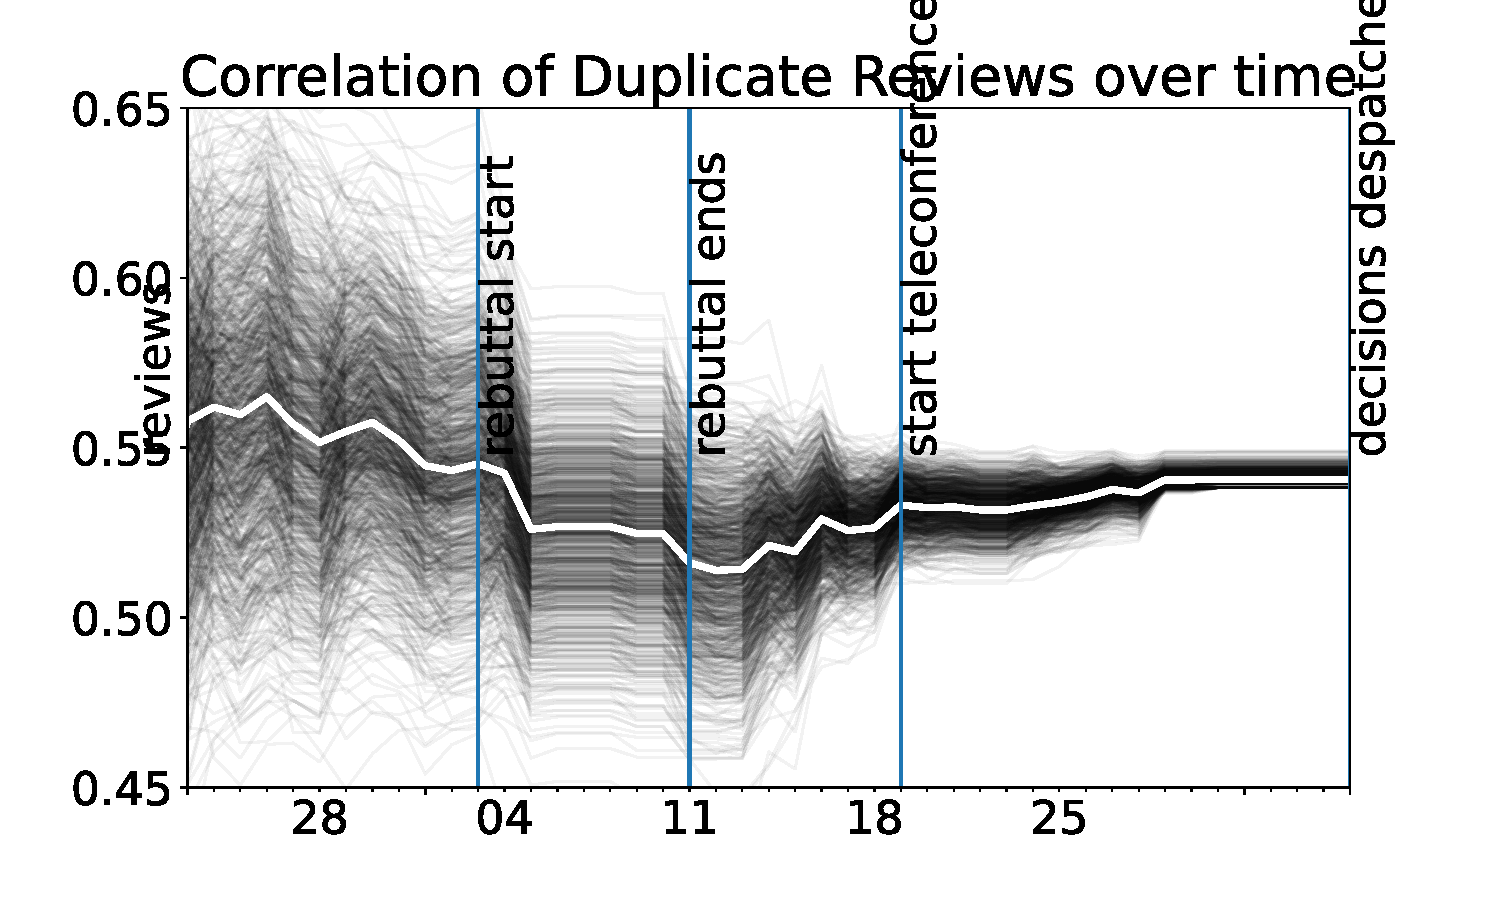
\includegraphics[width=0.70\textwidth]{diagrams/neurips/correlation-duplicate-reviews-bootstrap.pdf}


\caption{}
\label{correlation-duplicate-reviews-bootstrap}
\end{figure}

Plot the correlation of the duplicated papers over time (do bootstrap
samples here??)

\begin{figure}[htb]
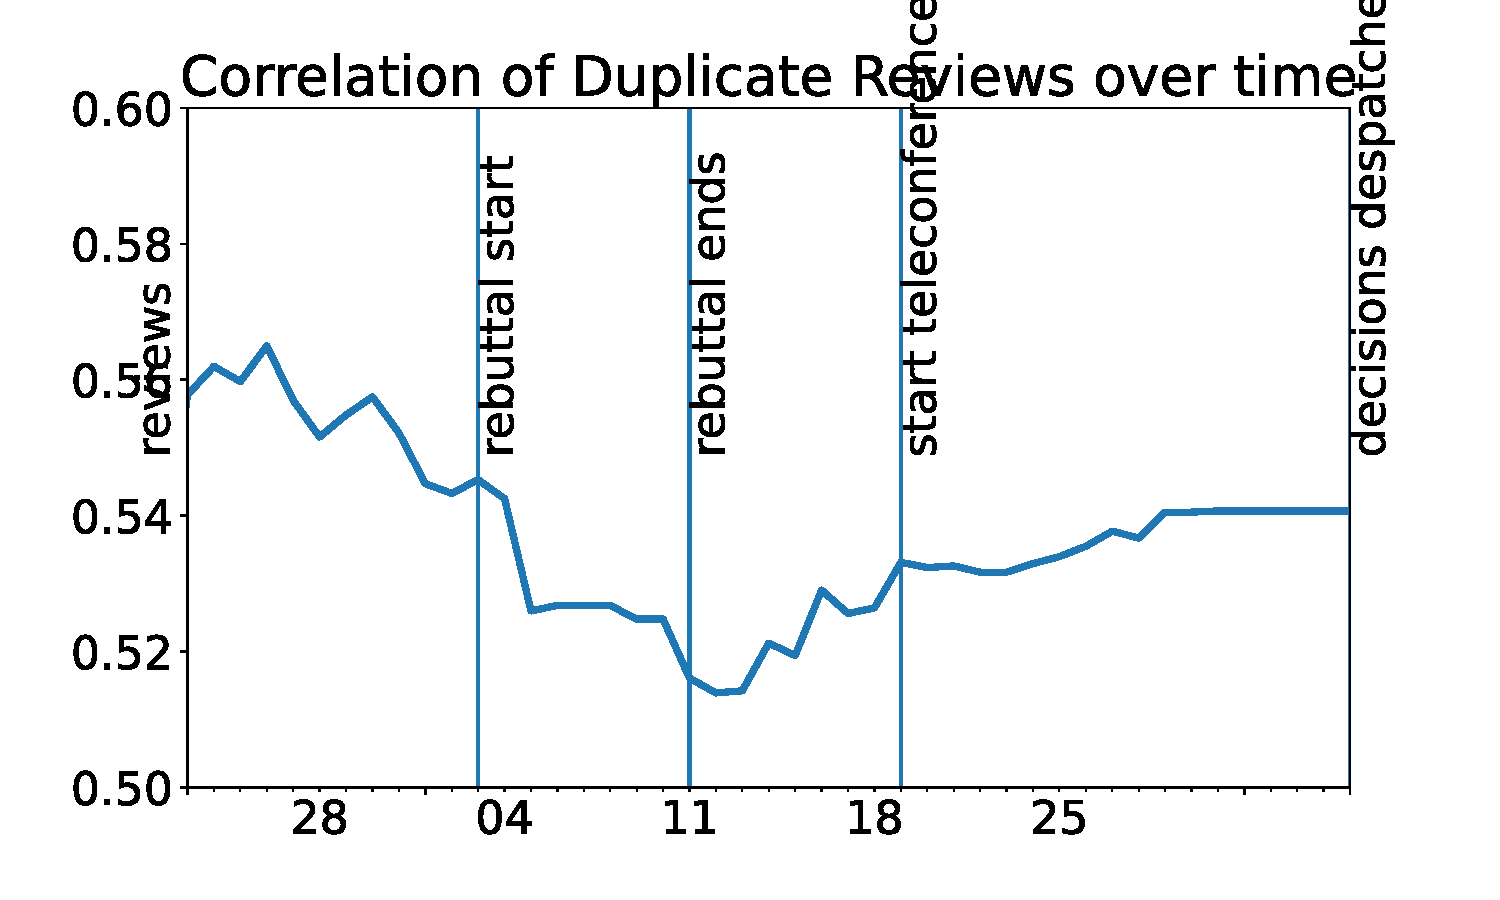
\includegraphics[width=0.70\textwidth]{diagrams/neurips/correlation-duplicate-reviews.pdf}


\caption{}
\label{correlation-duplicate-reviews}
\end{figure}

We need to do a bit more analysis on the estimation of the correlation
for the earlier submissions, but from what we see above, it looks like
the correlation is being damaged by late reviews, and we never quite
recover the consistency of reviews we had at the submission deadline
even after the discussion phase is over.

\hypertarget{late-reviewers-summary}{%
\subsection{Late Reviewers Summary}\label{late-reviewers-summary}}

In summary we find that late reviews are on average less confident and
shorter, but rate papers as higher quality and perhaps as higher impact.
Each of the effects is small (around 5\%) but overall a picture emerges
of a different category of review from those that delay their assesment.

\hypertarget{impact-of-papers-seven-years-on}{%
\subsection{Impact of Papers Seven Years
On}\label{impact-of-papers-seven-years-on}}

\begin{flushright}
[\href{https://github.com/lawrennd/talks/edit/gh-pages/_neurips/includes/impact-of-papers-seven-years-on.md}{edit}]
\end{flushright}

Now we look at the actual impact of the papers published using the
Semantic Scholar data base for tracking citations.

\begin{Shaded}
\begin{Highlighting}[]
\ImportTok{import}\NormalTok{ cmtutils }\ImportTok{as}\NormalTok{ cu}
\ImportTok{import}\NormalTok{ cmtutils.nipsy }\ImportTok{as}\NormalTok{ nipsy}
\ImportTok{import}\NormalTok{ cmtutils.plot }\ImportTok{as}\NormalTok{ plot}
\end{Highlighting}
\end{Shaded}

\begin{Shaded}
\begin{Highlighting}[]
\ImportTok{import}\NormalTok{ pandas }\ImportTok{as}\NormalTok{ pd}
\ImportTok{import}\NormalTok{ numpy }\ImportTok{as}\NormalTok{ np}
\end{Highlighting}
\end{Shaded}

\begin{Shaded}
\begin{Highlighting}[]
\NormalTok{papers }\OperatorTok{=}\NormalTok{ cu.Papers()}
\end{Highlighting}
\end{Shaded}

\url{https://proceedings.neurips.cc/paper/2014}

\begin{Shaded}
\begin{Highlighting}[]
\NormalTok{UPDATE\_IMPACTS }\OperatorTok{=} \VariableTok{False} \CommentTok{\# Set to True to download impacts from Semantic Scholar}
\end{Highlighting}
\end{Shaded}

The impact of the different papers is downloaded from Semantic scholar
using their REST API. This can take some time, and they also throttle
the calls. At the moment the code below deosn't handle the throttling
correctly. However, you it will load the cached version of of citations
scores from the given date.

\begin{Shaded}
\begin{Highlighting}[]
\ControlFlowTok{if}\NormalTok{ UPDATE\_IMPACTS:}
    \ImportTok{from}\NormalTok{ datetime }\ImportTok{import}\NormalTok{ datetime}
\NormalTok{    date}\OperatorTok{=}\NormalTok{datetime.today().strftime(}\StringTok{\textquotesingle{}\%Y{-}\%m{-}}\SpecialCharTok{\%d}\StringTok{\textquotesingle{}}\NormalTok{)}
\ControlFlowTok{else}\NormalTok{:}
\NormalTok{    date }\OperatorTok{=} \StringTok{"2021{-}06{-}11"}
\end{Highlighting}
\end{Shaded}

\begin{Shaded}
\begin{Highlighting}[]
\CommentTok{\# Rerun to download impacts from Semantic Scholar}
\ControlFlowTok{if}\NormalTok{ UPDATE\_IMPACTS:}
\NormalTok{    semantic\_ids }\OperatorTok{=}\NormalTok{ nipsy.load\_semantic\_ids()}
\NormalTok{    citations\_dict }\OperatorTok{=}\NormalTok{ citations.to\_dict(orient}\OperatorTok{=}\StringTok{\textquotesingle{}index\textquotesingle{}}\NormalTok{)}
    \CommentTok{\# Need to be a bit cleverer here. Semantic scholar will throttle this call.}
\NormalTok{    sscholar }\OperatorTok{=}\NormalTok{ nipsy.download\_citation\_counts(citations\_dict}\OperatorTok{=}\NormalTok{citations\_dict, semantic\_ids}\OperatorTok{=}\NormalTok{semantic\_ids)}
\NormalTok{    citations }\OperatorTok{=}\NormalTok{ pd.DataFrame.from\_dict(citations\_dict, orient}\OperatorTok{=}\StringTok{"index"}\NormalTok{) }
\NormalTok{    citations.to\_pickle(date }\OperatorTok{+} \StringTok{\textquotesingle{}{-}semantic{-}scholar{-}info.pickle\textquotesingle{}}\NormalTok{)}
\ControlFlowTok{else}\NormalTok{: }
\NormalTok{    citations }\OperatorTok{=}\NormalTok{ nipsy.load\_citation\_counts(date}\OperatorTok{=}\NormalTok{date)}
\end{Highlighting}
\end{Shaded}

The final decision sheet provides information about what happened to all
of the papers.

\begin{Shaded}
\begin{Highlighting}[]
\NormalTok{decisions }\OperatorTok{=}\NormalTok{ nipsy.load\_decisions()}
\NormalTok{nipsy.augment\_decisions(decisions)}
\end{Highlighting}
\end{Shaded}

This is joined with the citation information to provide our main ability
to understand the impact of these papers.

\begin{Shaded}
\begin{Highlighting}[]
\NormalTok{joindf }\OperatorTok{=}\NormalTok{ nipsy.join\_decisions\_citations(decisions, citations)}
\end{Highlighting}
\end{Shaded}

\hypertarget{correlation-of-quality-scores-and-citation}{%
\subsubsection{Correlation of Quality Scores and
Citation}\label{correlation-of-quality-scores-and-citation}}

Our first study will be to check the correlation between quality scores
of papers and how many times that the papers have been cited in
practice. In the plot below, rejected papers are given as crosses,
accepted papers are given as dots. We include all papers, whether
published in a venue or just available through ArXiv or other preprint
servers. We show the published/non-published quality scores and
\(\log_{10}(1+\text{citations})\) for all papers in the plot below. In
the plot we are showing each point corrupted by some Laplacian noise and
also removing axes. The idea is to give a sense of the distribution
rather than reveal the score of a particular paper.

\begin{figure}[htb]
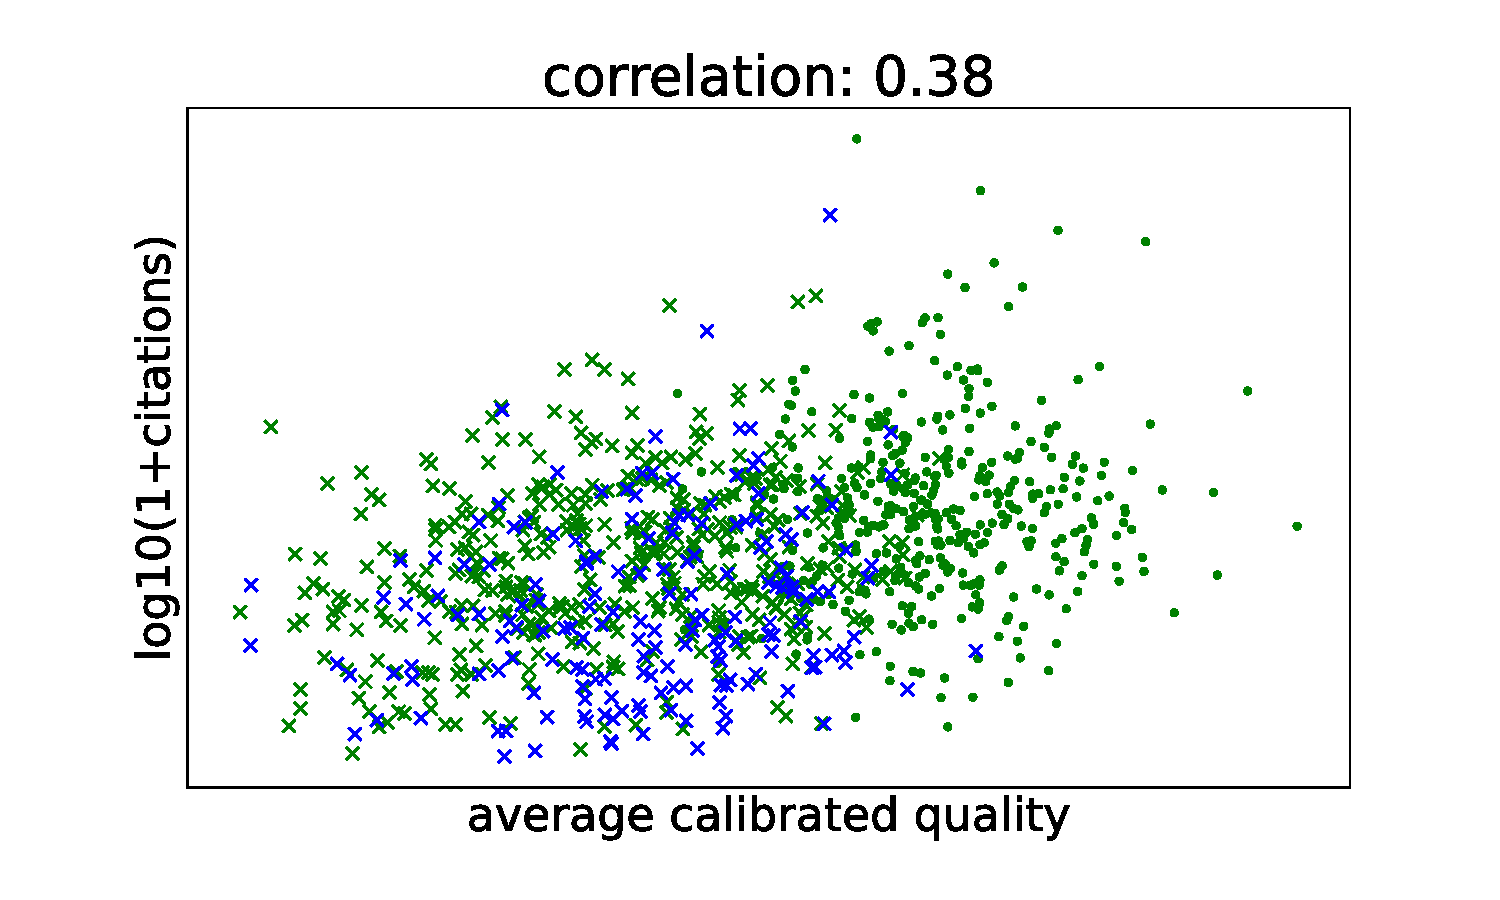
\includegraphics[width=0.70\textwidth]{diagrams/neurips/citations-vs-average-calibrated-quality-all.pdf}


\caption{}
\label{citations-vs-average-calibrated-quality-all}
\end{figure}

The correlation seems strong, but of course, we are looking at papers
which were accepted and rejected by the conference. This is dangerous,
as it is quite likely that presentation at the conference may provide
some form of lift to the papers' numbers of citations. So, the right
thing to do is to look at the groups separately.

Looking at the accepted papers only shows a very different picture.
There is very little correlation between accepted papers' quality scores
and the number of citations they receive.

\begin{figure}[htb]
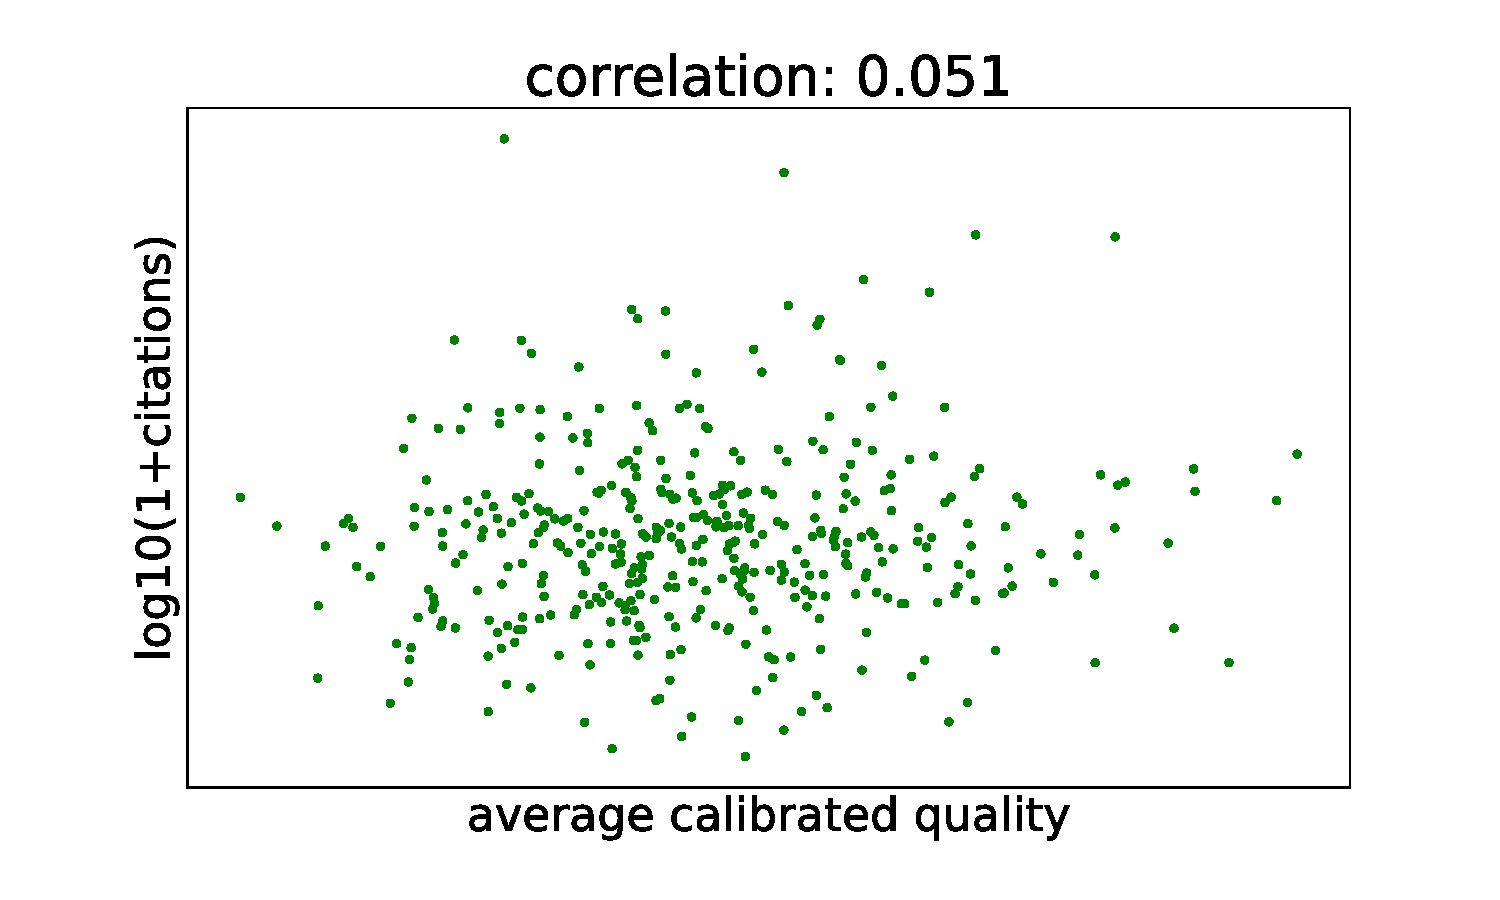
\includegraphics[width=0.70\textwidth]{diagrams/neurips/citations-vs-average-calibrated-quality-accept.pdf}


\caption{}
\label{citations-vs-average-calibrated-quality-accept}
\end{figure}

Conversely, looking at rejected papers only, we do see a slight trend,
with higher scoring papers achieving more citations on average. This,
combined with the lower average number of citations in the rejected
paper group, alongside their lower average scores, explains the
correlation we originally observed.

\begin{figure}[htb]
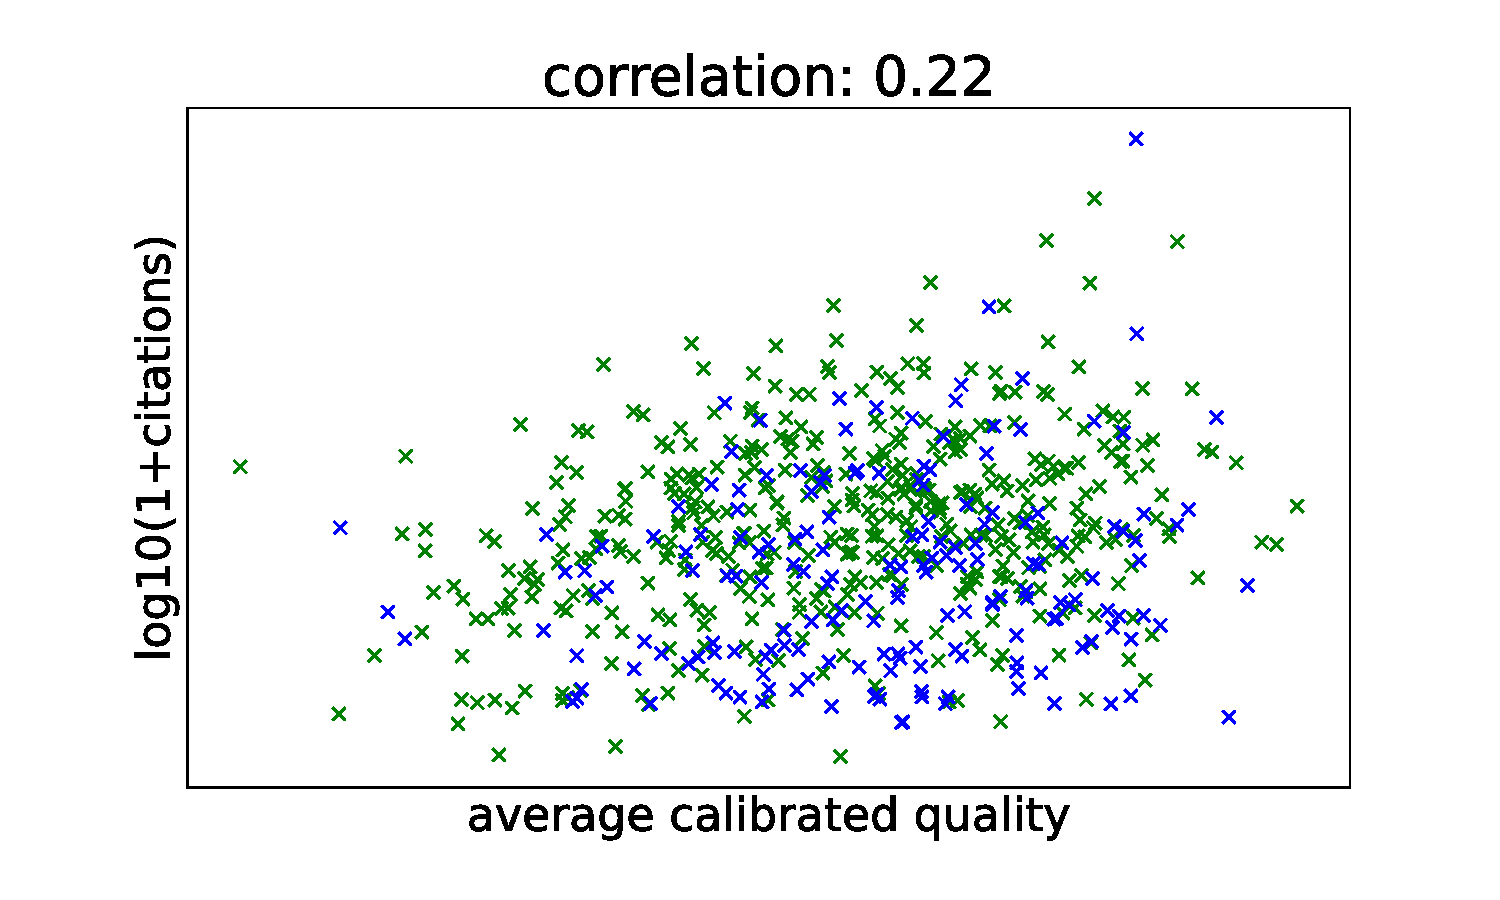
\includegraphics[width=0.70\textwidth]{diagrams/neurips/citations-vs-average-calibrated-quality-reject.pdf}


\caption{}
\label{citations-vs-average-calibrated-quality-reject}
\end{figure}

Welling and Ghahramani introduced an ``impact'' score in NeurIPS 2013,
we might expect the impact score to show correlation. And indeed,
despite the lower range of the score (a reviewer can score either 1 or
2) we do see \emph{some} correlation, although it is relatively weak.

\begin{figure}[htb]
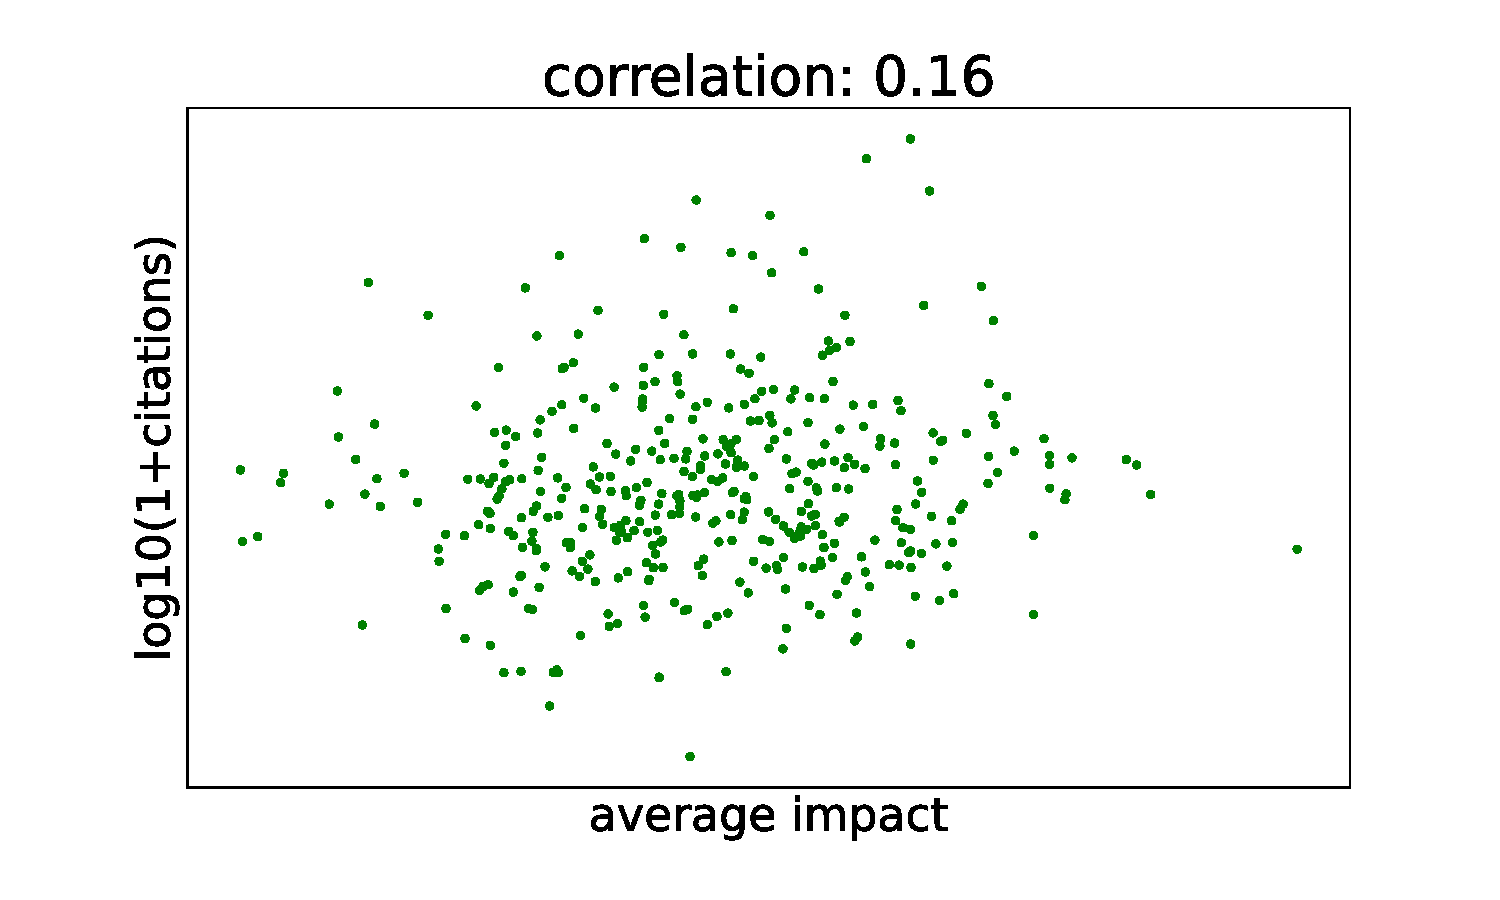
\includegraphics[width=0.70\textwidth]{diagrams/neurips/citations-vs-average-impact-accept.pdf}


\caption{}
\label{citations-vs-average-impact-accept}
\end{figure}

Finally, we also looked at correlation between the \emph{confidence}
score and the impact. Here correlation is somewhat stronger. Why should
confidence be an indicator of higher citations? A plausible explanation
is that there is confounder driving both variables. For example, it
might be that papers which are easier to understand (due to elegance of
the idea, or quality of exposition) inspire greater reviewer confidence
and also increase the number of citations.

\begin{figure}[htb]
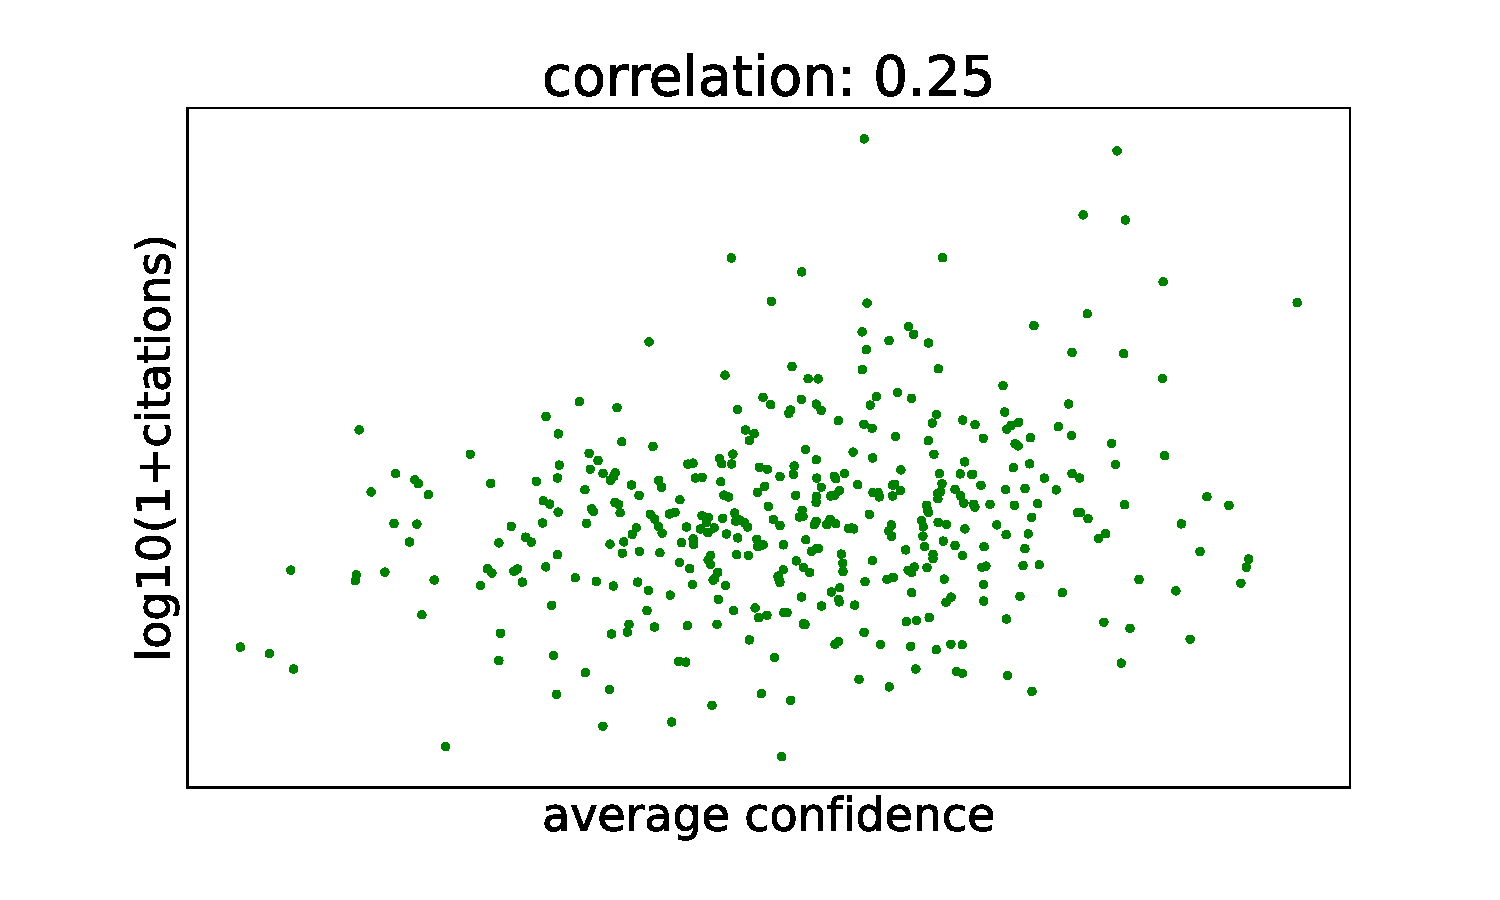
\includegraphics[width=0.70\textwidth]{diagrams/neurips/citations-vs-average-confidence-accept.pdf}


\caption{}
\label{citations-vs-average-confidence-accept}
\end{figure}

\begin{Shaded}
\begin{Highlighting}[]
\ControlFlowTok{for}\NormalTok{ column }\KeywordTok{in}\NormalTok{ [}\StringTok{"average\_quality"}\NormalTok{, }\StringTok{"average\_impact"}\NormalTok{, }\StringTok{"average\_confidence"}\NormalTok{]:}
\NormalTok{    cor }\OperatorTok{=}\NormalTok{ []}
    \ControlFlowTok{for}\NormalTok{ i }\KeywordTok{in} \BuiltInTok{range}\NormalTok{(}\DecValTok{1000}\NormalTok{):}
\NormalTok{        ind }\OperatorTok{=}\NormalTok{ bootstrap\_index(joindf.loc[joindf.accept])}
\NormalTok{        cor.append(joindf.loc[ind][column].corr(np.log(}\DecValTok{1}\OperatorTok{+}\NormalTok{joindf.loc[ind][}\StringTok{\textquotesingle{}numCitedBy\textquotesingle{}}\NormalTok{])))}
\NormalTok{    cora }\OperatorTok{=}\NormalTok{ np.array(cor)}
\NormalTok{    rho }\OperatorTok{=}\NormalTok{ cora.mean()}
\NormalTok{    twosd }\OperatorTok{=} \DecValTok{2}\OperatorTok{*}\NormalTok{np.sqrt(cora.var())}
    \BuiltInTok{print}\NormalTok{(}\StringTok{"}\SpecialCharTok{\{column\}}\StringTok{"}\NormalTok{.}\BuiltInTok{format}\NormalTok{(column}\OperatorTok{=}\NormalTok{column.replace(}\StringTok{"\_"}\NormalTok{, }\StringTok{" "}\NormalTok{)))}
    \BuiltInTok{print}\NormalTok{(}\StringTok{"Mean correlation is }\SpecialCharTok{\{rho\}}\StringTok{ +/{-} }\SpecialCharTok{\{twosd\}}\StringTok{"}\NormalTok{.}\BuiltInTok{format}\NormalTok{(rho}\OperatorTok{=}\NormalTok{rho, twosd}\OperatorTok{=}\NormalTok{twosd))}
\end{Highlighting}
\end{Shaded}

\hypertarget{conclusion}{%
\subsection{Conclusion}\label{conclusion}}

\begin{flushright}
[\href{https://github.com/lawrennd/talks/edit/gh-pages/_neurips/includes/neurips-experiment-conclusion.md}{edit}]
\end{flushright}

Under the simple model we have outlined, we can be confident that there
is inconsistency between two independent committees, but the level of
inconsistency is much less than we would find for a random committee. If
we accept that the bias introduced by the Area Chairs knowing when they
were dealing with duplicates was minimal, then if we were to revisit the
NIPS 2014 conference with an independent committee then we would expect
between \textbf{38\% and 64\% of the presented papers to be the same}.
If the conference was run at random, then we would only expect 25\% of
the papers to be the same.

It's apparent from comments and speculation about what these results
mean, that some people might be surprised by the size of this figure.
However, it only requires a little thought to see that this figure is
likely to be large for any highly selective conference if there is even
a small amount of inconsistency in the decision making process. This is
because once the conference has chosen to be `highly selective' then
because by definition only a small percentage of papers are to be
accepted. Now if we think of a type I error as accepting a paper which
should be rejected, such errors are easier to make because by definition
many more papers should be rejected. Type II errors (rejecting a paper
that should be accepted) are less likely becaue (by setting the accept
rate low) there are fewer papers that should be accepted in the first
place. When there is a difference of opinion between reviewers, it does
seem that many of the arugments can be distilled down to (a subjective
opinion) about whether controlling for type I or type II errors is more
important. Further, normally when discussing type I and type II errors
we believe that the underlying system of study is genuinely binary:
e.g.~diseased or not diseased. However, for conferences the
accept/reject boundary is not a clear separation point, there is a
continuum (or spectrum) of paper quality (as there also is for some
diseases). And the decision boundary often falls in a region of very
high density.

I would prefer a world were a conference is no longer viewed as a proxy
for research quality. The true test of quality is time. In the current
world, papers from conferences such as NeurIPS are being used to judge
whether a researcher is worthy of a position at a leading company, or
whether a researcher gets tenure. This is problematic and damaging for
the community. Reviewing is an inconsistent process, but that is not a
bad thing. It is far worse to have a reviewing system that is
consistently wrong than one which is inconsistently wrong.

My own view of a NeurIPS paper is inspired by the Millenium Galleries in
Sheffield. There, amoung the exhibitions they sometimes have work done
by apprentices in their `qualification'. Sheffield is known for knives,
and the work of the apprentices in making knives is sometimes very
intricate indeed. But it does lead to some very impractical knives.
NeurIPS seems to be good at judging technical skill, but not impact. And
I suspect the same is true of many other meetings. So, a publication a
NeurIPS does seem to indicate that the author has some of the skills
required, but it does not necessarily imply that the paper will be
impactful.

\hypertarget{thanks}{%
\subsection{Thanks!}\label{thanks}}

For more information on these subjects and more you might want to check
the following resources.

\begin{itemize}
\tightlist
\item
  twitter: \href{https://twitter.com/lawrennd}{@lawrennd}
\item
  podcast: \href{http://thetalkingmachines.com}{The Talking Machines}
\item
  newspaper:
  \href{http://www.theguardian.com/profile/neil-lawrence}{Guardian
  Profile Page}
\item
  blog:
  \href{http://inverseprobability.com/blog.html}{http://inverseprobability.com}
\end{itemize}

%%%%%%%%%%  End Body  %%%%%%%%%%


\vfill
\end{document}
